\PassOptionsToPackage{square,comma,numbers,sort&compress,super}{natbib}
\documentclass[12pt,twocolumn,twoside]{pnas-new}
% Use the lineno option to display guide line numbers if required.
% Note that the use of elements such as single-column equations
% may affect the guide line number alignment. 
%\usepackage{titling} % multiple title
\usepackage{balance} % balance last page of references
\usepackage{fancyvrb}


\usepackage{adjustbox}
\usepackage{setspace}

\usepackage{stackengine,scalerel}
%\usepackage{listings}


 
\def\useanchorwidth{F}
\def\stackalignment{r}%
\newcommand\overlap{\scalerel*{\hspace{.5mm}\stackinset{c}{-1.5pt}{c}{}{$O$}{$L$}}{+}}
 


\templatetype{pnasresearcharticle} % Choose template 
% {pnasresearcharticle} = Template for a two-column research article
% {pnasmathematics} = Template for a one-column mathematics article
% {pnasinvited} = Template for a PNAS invited submission

% \usepackage{bold-extra}
% \usepackage{setspace}
% \usepackage[margin=0.55in]{geometry}
% \usepackage{fullpage}
% \usepackage{rotating}
% \usepackage{pdflscape}

% \usepackage[scaled]{helvet}
% \renewcommand\familydefault{\sfdefault} 
% \usepackage[T1]{fontenc}
% \usepackage{upquote}

\usepackage{booktabs}
% \usepackage{algpseudocode}

%\usepackage[blue]{url}
\usepackage{subfig}
%\usepackage[12pt]{moresize}
\renewcommand{\marginpar}[1]{}

       %% \setlength{\oddsidemargin}{0.5in}
       %% \setlength{\evensidemargin}{0.5in}
       %% \setlength{\textwidth}{15cm}

\addtolength{\topmargin}{-0.7cm}
\addtolength{\textheight}{1.1cm}

\newcommand{\sub}[1]{\ensuremath{_{\mathsf{#1}}}} 
% \usepackage[usenames,dvipsnames,svgnames,table]{xcolor}

\usepackage{mathtools}
\usepackage{times}
%\usepackage{CJK}
\usepackage{latexsym}
\usepackage{multirow}
\usepackage{arydshln}

%% \newcommand*\circled[1]{\tikz[baseline=(char.base)]{
%%             \node[shape=circle,draw,inner sep=1pt] (char) {#1};}}
%% \usepackage[pdf]{pstricks}
%% \usepackage{pst-node,pst-coil}

\usepackage{graphicx}
\usepackage{ulem}	% to define \uline
\normalem

\usepackage{examples}
\exampleindent1.5em

\usepackage{float}

\usepackage{pdfpages}
\usepackage{xspace}
\usepackage{amssymb,amsmath,epsfig}
\usepackage{mathpartir}
\usepackage{amsthm}
\usepackage{mathrsfs}
%\usepackage{algorithm}
%\usepackage{pifont}
\usepackage{algorithmicx}
\usepackage[noend]{algpseudocode}

%\usetikzlibrary{matrix, positioning, arrows.meta, calc, shapes, decorations,  backgrounds, arrows, decorations.pathreplacing}
%\usepackage{pgfplots, siunitx}
\usepackage{hhline}

\newcommand{\nts}{\ensuremath{\text{\it nt}}\xspace}
\newcommand{\pairs}{\ensuremath{\mathrm{pairs}}\xspace}
\newcommand{\unpaired}{\ensuremath{\mathrm{unpaired}}\xspace}
\newcommand{\wunpaired}{\ensuremath{w_\text{unpaired}}\xspace}
\newcommand{\wcg}{\ensuremath{w_\text{CG}}\xspace}
\newcommand{\wgc}{\ensuremath{w_\text{GC}}\xspace}
\newcommand{\wau}{\ensuremath{w_\text{AU}}\xspace}
\newcommand{\wua}{\ensuremath{w_\text{UA}}\xspace}
\newcommand{\wgu}{\ensuremath{w_\text{GU}}\xspace}
\newcommand{\wug}{\ensuremath{w_\text{UG}}\xspace}
\newcommand{\ppv}{\ensuremath{\text{PPV}}\xspace}
\newcommand{\sens}{\ensuremath{\text{Sensitivity}}\xspace}
\newcommand*\rot{\rotatebox{90}}

\newcommand{\tuple}[1]{\ensuremath{\langle {#1} \rangle}}
\newcommand{\twotuple}[2]{\ensuremath{\langle {#1, #2} \rangle}}

%\newcommand{\argmax}[2]{\ensuremath{\mbox{argmax}_{#1}\ {#2}}}

\newcommand{\featuresum}[1]{\ensuremath{\sum_i \lambda_i f_i({#1})}}

\newcommand{\fvec}[1]{\ensuremath{\vec{f} ({#1})}}

\newcommand{\fiof}[1]{\ensuremath{f_i ({#1})}}

\newcommand{\fofi}[0]{\ensuremath{f_i}}

\newcommand{\featureprod}[1]
{\ensuremath{\vec{\lambda} \cdot \fvec{#1} } }

\newcommand{\efprod}[1]{\ensuremath{e^{\featureprod{#1}}}}
\newcommand{\efsum} [1]{\ensuremath{e^{\featuresum {#1}}}}

\newcommand{\lami}{\ensuremath{\lambda_i}}

\newcommand{\empExp}[1]{\ensuremath{\mbox{\~{E}} [{#1}]}}
\newcommand{\expect}{\ensuremath{\mathbb{E}}}

\newcommand{\ks}{\ensuremath{k}}
\newcommand{\Ks}{\ensuremath{K}}
\newcommand{\kbest}{\ks-best\xspace}
\newcommand{\best}{\ensuremath{\text{best}}\xspace}
\newcommand{\bestsc}{\ensuremath{\text{best\_score}}\xspace}

\newcommand{\topk}{top-\ks\xspace}
\newcommand{\kBest}{\Ks-Best\xspace}

\newcommand{\notes}[1]{}%{\it {\small {#1}}}}

\newcommand{\acite}[1]{({--#1})}

\newcommand{\define}[1]{{\bf Definition.} {\em {#1}}}
\newcommand{\zerobar}{\ensuremath{\overline{0}}\xspace}
\newcommand{\onebar}{\ensuremath{\overline{1}}\xspace}

\newcommand{\Items}{\ensuremath{\mathcal{I}}\xspace}

\newcommand{\oplusk}{\ensuremath{\oplus_{\tiny k}}}
\newcommand{\otimesk}{\ensuremath{\otimes_{\tiny k}}}

\newcommand{\zerok}{\ensuremath{\overline{0}^k}\xspace}
\newcommand{\onek}{\ensuremath{\overline{1}^k}\xspace}

\newcommand{\scalar}{\ensuremath{\odot_k}}

\newcommand{\kdim}{\ks-dimensional\ }





% \newlistof{defin}{def}{List of Definitions}

% \newcommand{\defin}[1]{%
% \refstepcounter{defin}
% \par\noindent\textbf{Definition \thedefin. #1}
% \addcontentsline{ans}{defin}{\protect\numberline{\thedefin}#1}\par}

% for amsthm
%  \theoremstyle{definition}
%  \newtheorem{definition}{Definition}
% \theoremstyle{plain}
% \newtheorem{theorem}{Theorem}
% \newtheorem{lemma}{Lemma}

%\newtheorem{theorem}{Theorem}[section]
%\newtheorem{definition}[theorem]{Definition}

\newcommand{\gc}{\ensuremath{|G|}\xspace}
\newcommand{\ntsize}{\ensuremath{|N|}\xspace}
\newcommand{\nt}{\ensuremath{N}\xspace}
\newcommand{\rulepernt}{\ensuremath{R}\xspace}

\newcommand{\Ttimesk}{\ensuremath{T_{\otimesk}}\xspace}
\newcommand{\Tplusk}{\ensuremath{T_{\oplusk}}\xspace}
\newcommand{\maxk}{\ensuremath{\mbox{\bf max}_k}\xspace}

\newcommand{\tenexp}[1]{\ensuremath{10^{{-#1}}}\xspace}

\newcommand{\naive}{na\"{\i}ve\xspace}

\newcommand{\perc}[1]{\ensuremath{{#1}\%}\xspace}

\newcommand{\veca}{\ensuremath{\mathbf{a}}}
\newcommand{\vecb}{\ensuremath{\mathbf{b}}}
\newcommand{\vecp}{\ensuremath{\mathbf{p}}}
\newcommand{\klogk}{\ensuremath{k\log k}}

\newcommand{\better}{\ensuremath{\preceq}}

\newcommand{\opt}{\ensuremath{\mbox{{\bf min}}_\better}}
\newcommand{\mergek}{\ensuremath{\mbox{{\bf merge}}_{\better k}}\xspace}
\newcommand{\multk}{\ensuremath{\mbox{{\bf mult}}_{\better k}}\xspace}

\newcommand{\kw}{\ensuremath{\mathbf{w}}}

\newcommand{\kwi}{\ensuremath{w_i}}
\newcommand{\wejv}[3]{\ensuremath{w^{#1}_{{#2}}({#3})}}

\newcommand{\vecj}{\ensuremath{\mathbf{j}}}
\newcommand{\vecD}{\ensuremath{\mathbf{D}}}
\newcommand{\vecu}{\ensuremath{\mathbf{u}}}
\newcommand{\vecU}{\ensuremath{\mathbf{U}}}
\newcommand{\vecjhat}{\ensuremath{\hat{\mathbf{j}}}}
\newcommand{\vecone}{\ensuremath{\mathbf{1}}}
\newcommand{\dbp}[2]{\ensuremath{\langle{#1}, {#2}\rangle}}

\newcommand{\reviewtimetoday}[3]{
    \AtBeginDocument{
    \special{
    !userdict begin
    /pagenum 0 def
    /bop-hook
    {
        /pagenum pagenum 1 add def
        pagenum #3 le
        {
        gsave
        430 750 translate
        0 rotate
        0.4 setgray
        /Times-Roman findfont
        10 scalefont setfont
        0 0   moveto
        (#1) show
        0 -10 moveto
        (#2) show
        grestore
        } if
    } def
    }  }}

% for submission
\iffalse
\renewcommand{\marginpar}[1]{}
\fi

% \newcommand{\comment}[1]{\marginpar{\raggedright{\em{\small #1}}}}

\newcommand{\ith}[1]{\ensuremath{i^{{th}}}}
\def\alglazy{Algorithm 3}

\newcommand{\JnM}{Jim\'enez and Marzal\xspace}

\newcommand{\ind}[1]{\ensuremath{^{(#1)}}}
\newcommand{\srule}[1]{\ensuremath{\mathrm{#1}}}
\newcommand{\goesto}{\ensuremath{\rightarrow}\xspace}
\newcommand{\chn}[1]{\mbox{{\it {#1}}}}

\newcommand{\ngramitem}[5]{
\ensuremath{
\left(
\begin{smallmatrix}
\mbox{\small {#4}} &\cdots & \mbox{\small {#5}} \\
&
%\!\!_{#2}
\mbox{#1}
%_{#3}
 &
\\ {#2} & & {#3}
\end{smallmatrix}
 \right)
}}

\newcommand{\specialngramitem}[7]{
\begin{math}
\left(
\begin{smallmatrix}
\mbox{\small {#2}}\ \cdots\ \mbox{\small{#3}}
& \cdots &
\mbox{\small {#4}}\ \cdots\ \mbox{\small {#5}} \\
& \mbox{{#1}} & \\
{#6} & & {#7}
\end{smallmatrix}
 \right)
\end{math}
}

\newcommand{\chartitem}[3]{
\ensuremath{(\mbox{#1},{#2},{#3})}
}

\newcommand{\vtnt}[1]{\ensuremath{V_{\mbox{\tiny #1}}}}
%%% \bigram{a}{b} means (a,b) is a bigram pair. P (b | a)!
\newcommand{\bigram}[2]{\ensuremath{\Pr(\mbox{\small #2} \mid \mbox{\small #1})}}

\newcount\permx
\newcount\permy
\def\permdot#1#2{
\permx=#1 \advance\permx by-1
\permy=#2 \advance\permy by-1
\psframe[fillcolor=black, fillstyle=solid]
(\permx,\permy)(#1, #2)
}

%%% note: realcalc.sty has a fatal bug : 23-0.5=23.5.
%%% so i have to do this... +1-0.5 thing
\newcommand{\minushalf}[1]{
    \Radd{\aaa}{#1}{-1}
    \Radd{\aaa}{\aaa}{0.5}
    \Rtrunc{\aaa}{1}{\aaa}
    \aaa
}


\newcommand{\permnt}[3]{
\rput({#1},{#2}){\huge\color{white} {#3}}
}


\newcommand\union{\cup}
\newcommand\intersect{\cap}

\newcommand\sign{\mathrm{sign}}

\newcommand\vecd[2]{\ensuremath{d_{#2}{(#1)}}}
\newcommand\veczero{\ensuremath{\mathbf{0}}}
\newcommand\vecq{\ensuremath{\mathbf{q}}}
\newcommand\vecn{\ensuremath{\mathbf{n}}}
%\newcommand\vecone{\ensuremath{\mathbf{1}}}
% \newcommand{\argmax}{\operatornamewithlimits{\mathbf{argmax}}}
\newcommand{\argtop}{\operatornamewithlimits{\mathbf{argtop}}}
\newcommand{\argmin}{\operatornamewithlimits{\mathbf{argmin}}}

\newcommand{\deltahat}{\ensuremath{\hat{\delta}}\xspace}

\newcommand{\xrs}{{\bf xRs}\xspace}
\newcommand{\xrsln}{\mbox{1-{\bf xRLNs}}\xspace}
\newcommand{\RLN}{{\bf RLN}\xspace}

% \newcommand{\x}[1]{\ensuremath{x_{#1}}\xspace}
\newcommand{\foot}[1]{\ensuremath{^{\tiny({#1})}_{\downarrow}}}


\newcommand{\chnprd}{{\tiny \ensuremath{_{\circ}}}}

%\newcommand{\ckyitem}[3]{\ensuremath{(_{#2}{\mbox{#1}}_{#3})}\xspace}
%\newcommand{\ckyitem}[3]{\ensuremath{({\mbox{#1}}_{#2, #3})}\xspace}
\newcommand{\ckyitem}[3]{\ensuremath{{\mbox{#1}}_{{{#2},\,{#3}}}}\xspace}
\newcommand{\treeitem}[2]{\ensuremath{{\mbox{#1}}_{#2}}\xspace}
\newcommand{\nodent}[3]{\ensuremath{\treeitem{#1}{#2}:{#3}}}

\newcommand{\coverage}[1]{\ensuremath{(\mbox{{#1}})}\xspace}
\newcommand{\lmcov}[2]{\ensuremath{(\mbox{#1}, ^{\mbox{#2}})}\xspace}
\newcommand{\phritem}[3]{\ensuremath{\coverage{#1}:({#2}, \mbox{``#3''})}\xspace}
\newcommand{\lmphritem}[4]{\ensuremath{\lmcov{#1}{#2}:({#3}, \mbox{``#4''})}\xspace}
\newcommand{\phrpair}[2]{\ensuremath{\langle \mbox{\chn{#1}, {#2}}\rangle}\xspace}

\newcommand{\lmitem}[3]{\ensuremath{({{#1}}^{#2 \star #3})}\xspace}
%\newcommand{\lmckyitem}[5]{\resizebox{!}{.15in}{\ensuremath{(\mbox{\small #1}_{\mbox{\tiny\ {#2},{#3}}}^{\tiny\ \mbox{#4}\ \star\ \mbox{#5}})}}\xspace}
\newcommand{\lmckyitem}[5]{\ensuremath{(\mbox{#1}_{\mbox{\scriptsize\ ({#2},{#3})}}^{\scriptsize\ \mbox{#4}\ \star\ \mbox{#5}})}\xspace}

\def\wlm{$\mathord+\textrm{LM}$\xspace}
\def\wolm{$\mathord-\textrm{LM}$\xspace}

\newcommand{\sym}[1]{\textrm{#1}\xspace}
\newcommand{\VP}{\sym{VP}}
\newcommand{\PP}{\sym{PP}}

\newcommand{\startsym}{\mbox{\texttt{<s>}}}
\newcommand{\stopsym}{\mbox{\texttt{</s>}}}
\newcommand{\TOP}{\sym{TOP}}
%\newcommand{\plm}[2]{\ensuremath{P_{lm}(\mbox{\small #2}\mid\mbox{\small #1})}}
\newcommand{\plm}[2]{\ensuremath{P_{lm}(\mbox{#2}\mid\mbox{#1})}}

%\newcommand{\order}[1]{\ensuremath{\mathcal{O}(#1)}}
\newcommand{\order}{\ensuremath{\mathcal{O}}}

\newcommand{\wocombo}{\ensuremath{h}\xspace}
\newcommand{\mincombo}{\ensuremath{h_{\mathit{combo}}}\xspace}

%\renewcommand{\min}{\ensuremath{\mbox{\bf min}}\xspace}
\newcommand{\hyp}[1]{\mbox{\tiny ``{#1}''}}
\newcommand{\hl}{\ensuremath{k}\xspace}


\newcommand{\cand}{\ensuremath{\mathit{cand}}\xspace}
\newcommand{\buf}{\ensuremath{\mathit{buf}}\xspace}
\newcommand{\bound}{\ensuremath{\mathit{bound}}\xspace}

\newcommand{\lazyjbest}{\ensuremath{\textproc{LazyJthBest}}\xspace}

\newcommand{\backwardstar}{\ensuremath{\mathit{IN}}\xspace}

% \newtheorem{proposition}[theorem]{Proposition}

\newcommand{\ff}{\ensuremath{\mathbf{f}}\xspace}
\newcommand{\ee}{\ensuremath{\mathbf{e}}\xspace}
\newcommand{\al}{\ensuremath{\mathbf{a}}\xspace}

\newcommand{\pt}{\ensuremath{p_{\mbox{t}}}}
\newcommand{\pd}{\ensuremath{p_{\mbox{d}}}}


\newcommand{\current}{\color{blue}{\fbox{{\bf C}}}\xspace}
\newcommand{\future}{\color{red}{\fbox{{\bf F}}}\xspace}

%\newcommand{\ind}[1]{\ensuremath{^{\kern-0.5pt\boxnum{#1}}}}
\newcommand{\BS}{\ensuremath{\mathit{IN}}\xspace}

\def\FS{\mathit{FS}\xspace}
\def\BS{\mathit{BS}\xspace}
\def\bfR{\mathbf{R}\xspace}

\newcommand{\head}{\ensuremath{\mathit{head}}\xspace}
\newcommand{\tails}{\ensuremath{\mathit{tails}}\xspace}

\newcommand{\Deriv}{\ensuremath{\mathscr{D}}\xspace}
\newcommand{\hhat}{\ensuremath{\hat{h}}\xspace}

\newcommand{\opluseq}{\ensuremath{\ \oplus=}\xspace}

\newcommand{\chnyu}{\chn{y\v{u}}\xspace}
\newcommand{\chnle}{\chn{le}\xspace}
\newcommand{\chnShalong}{\chn{Sh\=al\'ong}\xspace}
\newcommand{\chnBaoweier}{\chn{B\`aow\=eier}\xspace}
\newcommand{\chnjuxing}{\chn{j\v{u}x\'ing}\xspace}
\newcommand{\chnhuitan}{\chn{hu\`it\'an}\xspace}

\newcommand{\mybullet}{\ensuremath{\bullet\hspace{-0.05mm}}}
\newcommand{\myunderscore}{\ensuremath{\mbox{\Large\_}}}
\newcommand{\halfcov}{\myunderscore\myunderscore\mybullet\mybullet\mybullet}
\newcommand{\fullcov}{\mybullet\mybullet\mybullet\mybullet\mybullet}
\newcommand{\fullncov}{\mybullet\mybullet\ldots\mybullet}


\long\def\signature#1{%
% \begin{flushleft}
\begin{center}
% \begin{minipage}{6in}
\parindent=0pt
\shortstack{\vrule width 3in height 0.4pt\\ #1}
% \end{minipage}
\end{center}
% \end{flushleft}
}

% forest rerank acl 2008
\newcommand{\feat}[1]{{\bf {#1}}}
\newcommand{\Gen}[1]{\ensuremath{\mathit{cand}({#1})}\xspace}
\newcommand{\yhat}{\ensuremath{\hat{y}}\xspace}
\newcommand{\ystar}{\ensuremath{y^*}\xspace}
\newcommand{\yplus}{\ensuremath{y^+}\xspace}
\newcommand{\score}{\ensuremath{\mathit{sc}}\xspace}
\newcommand{\cost}{\ensuremath{\mathit{c}}\xspace}
\newcommand{\oracle}{\ensuremath{\mathit{oracle}}\xspace}
\newcommand{\ora}{\ensuremath{\mathit{ora}}\xspace}
\newcommand{\cnj}{charniak+johnson:2005}
\newcommand{\coll}{collins:2000}
\newcommand{\dom}{\ensuremath{\mathit{dom}}\xspace}
\newcommand{\gold}{\ensuremath{\mathit{gold}}\xspace}

\newcommand{\myoval}[1]{\ovalnode[linestyle=none,fillstyle=solid,fillcolor=lightgray]{foo}{#1}}
\newcommand{\myboxmath}[1]{\ensuremath{\fcolorbox{white}{lightgray}{\!\ensuremath{#1}\!}}\xspace}
\newcommand{\myboxmathsub}[1]{\scalebox{0.75}{\ensuremath{\fcolorbox{white}{lightgray}{\!\ensuremath{#1}\!}}}\xspace}
\newcommand{\myboxedgemath}[1]{\ensuremath{\fcolorbox{black}{lightgray}{\!\ensuremath{#1}\!}}\xspace}
\newcommand{\mybox}[1]{\ensuremath{\fcolorbox{white}{lightgray}{\!{#1}\!}}\xspace}
\newcommand{\mybluebox}[1]{\ensuremath{\fcolorbox{white}{cyan}{\!{#1}\!}}\xspace}
\newcommand{\mymagentabox}[1]{\ensuremath{\fcolorbox{white}{magenta}{\!{#1}\!}}\xspace}
\newcommand{\mypinkbox}[1]{\ensuremath{\fcolorbox{white}{pink}{\!{#1}\!}}\xspace}
\newcommand{\myyellowbox}[1]{\ensuremath{\fcolorbox{white}{yellow}{\!{#1}\!}}\xspace}
\newcommand{\myorangebox}[1]{\ensuremath{\fcolorbox{white}{orange}{\!{#1}\!}}\xspace}
\newcommand{\mygreenbox}[1]{\ensuremath{\fcolorbox{white}{green}{\!{#1}\!}}\xspace}
\newcommand{\myboxedge}[1]{\ensuremath{\fcolorbox{black}{lightgray}{\!{#1}\!}}\xspace}

%\newcommand{\mybox}[1]{\psframebox[linestyle=none,linewidth=0pt,fillstyle=solid,fillcolor=lightgray]{#1}}

\newcommand{\vecx}{\ensuremath{\mathbf{x}}\xspace}
\newcommand{\vecy}{\ensuremath{\mathbf{y}}\xspace}
\newcommand{\vecw}{\ensuremath{\mathbf{w}}\xspace}

\newcommand{\vecystar}{\ensuremath{\vecy^*}\xspace}
\newcommand{\vecyhat}{\ensuremath{\hat{\vecy}}\xspace}
\newcommand{\vecybar}{\ensuremath{\bar{\vecy}}\xspace}
\newcommand{\valid}{\ensuremath{\mathrm{valid}}\xspace}
\newcommand{\balanced}{\ensuremath{\mathrm{balanced}}\xspace}
\newcommand{\depth}{\ensuremath{\mathrm{depth}}\xspace}

\newcommand{\scorew}{\ensuremath{\mathit{sc}_{\vecw}}\xspace}

\newcommand{\vecv}{\ensuremath{\mathbf{v}}\xspace}
\newcommand{\vecf}{\ensuremath{\mathbf{f}}\xspace}
\newcommand{\vecfl}{\ensuremath{\mathbf{f}_L}\xspace}
%\newcommand{\veczero}{\ensuremath{\mathbf{j}}}

\newcommand{\heap}{\ensuremath{\mathit{heap}}\xspace}

\newcommand{\feature}[1]{$\langle$ {#1} $\rangle$\xspace}

\newcommand{\defineq}{\ensuremath{\; \triangleq\; }\xspace}
\newcommand{\extradgt}{\color{white}{0}\xspace}

\newcommand{\funit}{\ensuremath{\mathring{f}}\xspace}
\newcommand{\vecfunit}{\ensuremath{\mathring{\vecf}}\xspace}
\newcommand{\Done}[1]{\ensuremath{D_1(#1)}}

% kbest paper 2005
\let\algsize\normalsize
\newcommand{\algline}[2]{%
\begin{center}
\algsize$\text{#1:}\hspace{1em}#2$
\end{center}}

\def\Dhat{\hat{D}}
\def\vecDhat{\mathbf{\hat{D}}}

%%%%%%%%%%%%%%% pinyins

\newcommand{\Baoweier}{\chn{B\`aow\=eier}\xspace}
\newcommand{\Bushi}{\chn{B\`ush\'i}\xspace}
\newcommand{\Shalong}{\chn{Sh\=al\'ong}\xspace}
\newcommand{\yu}{\chn{y\v{u}}\xspace}
\newcommand{\hai}{\chn{h\'ai}\xspace}
\newcommand{\jiang}{\chn{ji\=ang}\xspace}
\newcommand{\huiwu}{\chn{hu\`iw\`u}\xspace}
\newcommand{\jinyibu}{\chn{j\`iny\={\i}b\`u}\xspace}
\newcommand{\juxing}{\chn{j\v{u}x\'ing}\xspace}
\newcommand{\huitan}{\chn{hu\`it\'an}\xspace}
\newcommand{\dangtian}{\chn{d\=angti\=an}\xspace}
\newcommand{\jiu}{\chn{ji\`u}\xspace}
\newcommand{\zhongdong}{\chn{zh\=ongd\=ong}\xspace}
\newcommand{\weiji}{\chn{w\=eij\=\i}\xspace}
\newcommand{\fuze}{\chn{f\`uz\'e}\xspace}

\newcommand{\Prob}{\ensuremath{\mathrm{P}}\xspace}

\newcommand{\lhs}{\ensuremath{\mathit{lhs}}\xspace}
\newcommand{\rhs}{\ensuremath{\mathit{rhs}}\xspace}

\newcommand{\NULL}{\ensuremath{\mathit{null}}\xspace}

\newcommand{\gap}{\ensuremath{\sqcup}\xspace}
\newcommand{\spanof}{\ensuremath{\mathit{span}}\xspace}
\newcommand{\yield}{\ensuremath{\mathit{yield}}\xspace}
\newcommand{\fs}{\ensuremath{\mathit{admset}}\xspace}

\newcommand{\closed}{\ensuremath{\mathit{closed}}\xspace}
\newcommand{\open}{\ensuremath{\mathit{open}}\xspace}
\newcommand{\hs}{\frag} %\ensuremath{\mathit{frag}}\xspace}
\newcommand{\vs}{\ensuremath{\mathit{vs}}\xspace}
\newcommand{\frag}{\ensuremath{\mathit{frag}}\xspace}
\renewcommand{\root}{\ensuremath{\mathit{root}}\xspace}
\newcommand{\leaves}{\yield} %\ensuremath{\mathit{leaves}}\xspace}
\newcommand{\exps}{\ensuremath{\mathit{front}}\xspace} % frontier
\newcommand{\newexps}{\ensuremath{\mathit{\exps'}}\xspace}


\newcommand{\PLM}{\ensuremath{\Prob_{\mathrm{lm}}}\xspace}
\newcommand{\PT}{\ensuremath{\Prob}\xspace}
\newcommand{\PLex}{\ensuremath{\Prob_{\mathrm{lex}}}\xspace}

\newcommand{\GHKM}[3]{\ensuremath{{\mbox{#1}}_{{#2}}^{{#3}}}\xspace}
%\newcommand{\newGHKM}[2]{\ensuremath{{\mbox{#1}}\\{\mbox{\scriptsize #2}}}\xspace}
\newcommand{\tspan}[1]{\scriptsize {#1}\xspace}
\newcommand{\wnode}[1]{\rnode[t]{#1}{#1}\xspace}  %% target words

\newcommand{\vtitem}[2]{\ensuremath{({\vtnt{#1}}_{#2})}\xspace}
%\newcommand{\gap}{\ensuremath{\sqcup}}
%\newcommand{\treeitem}[2]{\ensuremath{({\mbox{#1}}_{#2})}\xspace}

\newcommand{\ruleset}{\ensuremath{\mathcal{R}}\xspace}

% pattern-match
\newcommand{\match}{\ensuremath{\mathit{match}}\xspace}
\newcommand{\vars}{\ensuremath{\mathit{vars}}\xspace}
\newcommand{\mlist}{\ensuremath{\mathit{mlist}}\xspace}
%\newcommand{\Prob}{\ensuremath{\mathrm{P}}\xspace}
\newcommand{\eP}{\ensuremath{e_{\mathit{p}}}\xspace}
%\newcommand{\PLM}{\ensuremath{\Prob_{\mathrm{lm}}}\xspace}
% \newcommand{\PT}{\ensuremath{\Prob}\xspace}
% \newcommand{\PLex}{\ensuremath{\Prob_{\mathrm{lex}}}\xspace}

%NOW MOVED HERE
\newcommand{\npshift}{\hspace{1.6cm}}
\newcommand{\styleb}{linestyle=dashed}

\newcommand{\et}{\ensuremath{e^{\mathrm{t}}}}
\newcommand{\Ht}{\ensuremath{H^{\mathrm{t}}}}
%\newcommand{\ep}{\ensuremath{e^{\mathrm{p}}}}
\newcommand{\ep}{\ensuremath{e}\xspace}  % just for EMNLP
\newcommand{\Hp}{\ensuremath{H^{\mathrm{p}}}}
\newcommand{\Vp}{\ensuremath{V^{\mathrm{p}}}}



\def\Fone{F$_1$\xspace}
\def\Foneperc{F$_1\%$}
\newcommand{\goto}{\ensuremath{\triangleright}\xspace}

\newcommand{\TODO}[1]{\textbf{TODO:} \textit{#1}\xspace}

\newcommand{\smallnt}[1]{\ensuremath{_{\mbox{\tiny PP}}}\xspace}

\newcommand{\shift}{\ensuremath{\mathsf{sh}}\xspace}
\newcommand{\reduce}{\ensuremath{\mathsf{re}}\xspace}
\newcommand{\lreduce}{\ensuremath{\mathsf{re_{\small \curvearrowleft}}}\xspace}
\newcommand{\rreduce}{\ensuremath{\mathsf{re_{\small \curvearrowright}}}\xspace}


\newcommand{\sep}{\ensuremath{ \circ }\xspace}

\newcommand{\sttop}{\ensuremath{s_0}\xspace}
\newcommand{\stnext}{\ensuremath{s_1}\xspace}
\newcommand{\stthird}{\ensuremath{s_2}\xspace}
\newcommand{\qhead}{\ensuremath{q_0}\xspace}
\newcommand{\qnext}{\ensuremath{q_1}\xspace}
\newcommand{\qthird}{\ensuremath{q_2}\xspace}
\newcommand{\Tag}[1]{\ensuremath{{#1}.\mathsf{t}}\xspace}
\newcommand{\Wrd}[1]{\ensuremath{{#1}.\mathsf{w}}\xspace}
\newcommand{\LC}[1]{\ensuremath{{#1}.\mathsf{lc}}\xspace}
\newcommand{\RC}[1]{\ensuremath{{#1}.\mathsf{rc}}\xspace}

% Algorithm 3 -> Pseudocode 3
\newcommand{\pseudocode}{Algorithm}
% \floatname{algorithm}{\pseudocode}

\newcommand{\cont}[2]{\ensuremath{\mathit{c}({#1}, {#2})}\xspace}
\newcommand{\contR}[2]{\ensuremath{\mathit{c}_{\mbox{\tiny \sc R}}({#1}, {#2})}\xspace}
\newcommand{\contsttops}{\ensuremath{\cont{\stnext}{\sttop}}\xspace}
\newcommand{\contsttopqhead}{\ensuremath{\contR{\sttop}{\qhead}}\xspace}

\newcommand{\sspan}{\ensuremath{\mathit{sp}}\xspace}
\renewcommand{\tspan}{\ensuremath{\mathit{tp}}\xspace}
\newcommand{\aspan}{\ensuremath{\mathit{ap}}\xspace}

% vanilla non-dp shift-reduce item: (l, S, Q)
\newcommand{\olditem}[3]{\ensuremath{{#1}: \tuple{{#2}, \ {#3}}}\xspace}
%\newcommand{\newitem}[4]{\ensuremath{{#1}: \tuple{{#2}, \ {#3}, \ {#4}}}\xspace}
\newcommand{\newitem}[3]{\ensuremath{\tuple{{#1},  {#2},  {#3}}}\xspace}

\newcommand{\arcs}{\ensuremath{\mathbf{a}}\xspace}
%\newcommand{\arcleft}[2]{\ensuremath{\mbox{#1}^\curvearrowleft\mbox{#2}}\xspace}
\newcommand{\arcleft}[2]{{#1}$^\curvearrowleft${#2}\xspace}
%\newcommand{\arcright}[2]{\ensuremath{\mbox{#1}^\curvearrowright\mbox{#2}}\xspace}
\newcommand{\arcright}[2]{{#1}$^\curvearrowright${#2}\xspace}

%\newcommand{\score}{\ensuremath{\mathit{sc}}\xspace}
\newcommand{\scoring}[2]{\ensuremath{\score_{#1}({#2})}\xspace}
\newcommand{\scoreshift}[1]{\ensuremath{\scoring{\shift}{#1}}\xspace}
\newcommand{\scoreleft}[1]{\ensuremath{\scoring{\lreduce}{#1}}\xspace}
\newcommand{\scoreright}[1]{\ensuremath{\scoring{\rreduce}{#1}}\xspace}
\newcommand{\scorereduce}[1]{\ensuremath{\scoring{\reduce}{#1}}\xspace}


%% \newcommand{\arcleft}[2]{\ensuremath{{#1}^\curvearrowleft{#2}}\xspace}
%% \newcommand{\arcright}[2]{\ensuremath{{#1}^\curvearrowright{#2}}\xspace}

% kernel feature function
\newcommand{\vecfker}{\ensuremath{\widetilde{\mathbf{f}}}\xspace}
\newcommand{\fker}[1]{\ensuremath{\vecfker({#1})}\xspace}
\newcommand{\earleyitem}[3]{\ensuremath{\tuple{{#1}, {#2}, \ {#3}}}\xspace}
\newcommand{\nodpearleyitem}[2]{\ensuremath{\tuple{{#1}, \ {#2}}}\xspace}

\iffalse
\newcommand{\eisneritem}[4]{\newitem{#1}{#2}{#3}{\!\!\!\raisebox{0.04in}{\Tree[.{\ensuremath{#4}} !\Troof{\ensuremath{{#2}...{#3}}} ]}}\xspace}
\newcommand{\specialeisneritem}[4]{\newitem{#1}{#2}{#3}{#4}\xspace}
\else
\newcommand{\eisneritem}[4]{\tuple{{#1}, {\!\!\!\raisebox{0.04in}{\Tree[.{\ensuremath{#4}} !\Troof{\ensuremath{{#2}...{#3}}} ]}}\!\!\!}\xspace}
\newcommand{\specialeisneritem}[4]{\ensuremath{{#1}: \tuple{{#4}}}\xspace}
\newcommand{\gpeisneritem}[5]{\ensuremath{{#1}:\tuple{{#4}, {\!\!\!\raisebox{0.04in}{\Tree[.{\ensuremath{#5}} !\Troof{\ensuremath{{#2}...{#3}}} ]}}\!\!\!}}\xspace}
\fi

\newcommand{\decode}{\ensuremath{\mathit{decode}}\xspace}
\newcommand{\GEN}{\ensuremath{\mathcal{Y}}\xspace}
\newcommand{\GENbar}{\ensuremath{\overline{\GEN}}\xspace}

\newcommand{\BLEU}{\ensuremath{\mathrm{BLEU}\xspace}}
\newcommand{\BLEUplusone}{\ensuremath{\mathrm{BLEU}_{+1}\xspace}}

\newcommand{\spb}[1]{\ensuremath{^{({#1})}}\xspace}
\newcommand{\spbkp}{\ensuremath{\spb{k+1}}\xspace}
\newcommand{\vecwk}{\ensuremath{\vecw\spb{k}}\xspace}
\newcommand{\vecwkp}{\ensuremath{\vecw\spb{k+1}}\xspace}


\newcommand{\err}{\ensuremath{\mathit{err}}\xspace}
\newcommand{\bPhi}{\ensuremath{\mathbf{\Phi}}\xspace}
\newcommand{\dPhi}{\ensuremath{\Delta\bPhi}\xspace}
\newcommand{\labels}{\ensuremath{\mathit{labels}}\xspace}
\newcommand{\onestep}{\ensuremath{\mathit{onestep}}\xspace}
\newcommand{\seqx}{\ensuremath{\overline{x}}\xspace}
\newcommand{\seqy}{\ensuremath{\overline{y}}\xspace}
\newcommand{\seqz}{\ensuremath{\overline{z}}\xspace}

\providecommand{\norm}[1]{\lVert#1\rVert}
\newcommand{\normtwo}[1]{\norm{#1}^2}

\newcommand{\seqzt}{\ensuremath{\overline{z}^{(t)}}\xspace}
\newcommand{\seqxt}{\ensuremath{\overline{x}^{(t)}}\xspace}
\newcommand{\seqyt}{\ensuremath{\overline{y}^{(t)}}\xspace}

\newcommand{\defeq}{\ensuremath{\stackrel{\Delta}{=}}\xspace}
\newcommand{\InlineIf}[2]{{\bf if} {#1} {\bf then} {#2}}
\newcommand{\dsep}{\ensuremath{\mathcal{D}(\vecu,\delta)}\xspace}
\newcommand{\dgsep}{\ensuremath{\mathcal{D}_g(\vecu,\delta)}\xspace}

\newcommand{\hinge}{\ensuremath{h_{\delta}}\xspace}

\newcommand{\Beam}{\ensuremath{\mathcal{B}}\xspace}

% equivalence class under ~: [[x]]_~
\newcommand{\eqvcls}[1]{\ensuremath{\llbracket {#1} \rrbracket_{\equiv}}\xspace}

\newcommand{\Cs}{\ensuremath{C_{\mathrm{s}}}}
\newcommand{\Cg}{\ensuremath{C_{\mathrm{g}}}}
\newcommand{\Cb}{\ensuremath{C_{\mathrm{b}}}}
 
%lhuang
%\renewcommand{\subsubsection}[1]{\vspace{0.5cm}\noindent{\bf {#1}.}\hspace{0.2cm}}
%\newcommand{\viol}[4]{\ensuremath{\mathcal{V}_{{#4}}(#1, #2, #3)}\xspace}
\newcommand{\viol}[1]{\ensuremath{\mathcal{V}_{{#1}}}\xspace}

\newcommand{\bleu}{{\sc Bleu}\xspace}
%\newcommand{\mert}{{\sc Mert}\xspace}
\newcommand{\pro}{{\sc Pro}\xspace}
\newcommand{\mira}{{\sc Mira}\xspace}
\newcommand{\hols}{{\sc Hols}\xspace}
\newcommand{\ramp}{{\sc Ramp}\xspace}

\newcommand{\myinfer}[3]{\ensuremath{\infer[\mbox{\footnotesize ${#1}$}]{#2}{#3}}\xspace}
\newcommand{\pre}{\ensuremath{\mathit{pre}}\xspace}
\newcommand{\good}{\ensuremath{\mathit{good}}\xspace}
\newcommand{\bad}{\ensuremath{\mathit{bad}}\xspace}
\newcommand{\ygood}{\ensuremath{\mbox{$y$-good}}\xspace}
\newcommand{\ybad}{\ensuremath{\mbox{$y$-bad}}\xspace}

\newcommand{\Predict}{\ensuremath{\mbox{\sc \footnotesize Pred}}\xspace}
\newcommand{\Complete}{\ensuremath{\mbox{\sc \footnotesize Comp}}\xspace}

\newcommand{\leftptrs}{\ensuremath{\mathcal{L}}\xspace}


\newcommand{\Loss}{\ensuremath{\mathcal{L}}\xspace}
\newcommand{\loss}{\ensuremath{\ell}\xspace}

\newcommand{\subtype}{\ensuremath{<:}}
\newcommand{\type}[1]{\ensuremath{\mathsf{{#1}}}\xspace}

\newcommand{\geoquery}{\ensuremath{\textsc{GeoQuery}}\xspace}
\newcommand{\jobs}{\ensuremath{\textsc{Jobs}}\xspace}
\newcommand{\atis}{\ensuremath{\textsc{ATIS}}\xspace}
\newcommand{\tv}[1]{\ensuremath{\mbox{\tt \textquotesingle}\!\text{\tt{#1}}}}
\newcommand{\tva}{\ensuremath{\tv{a}}\xspace}

\newcommand{\var}[1]{\ensuremath{{#1}}}
\newcommand{\pred}[1]{\ensuremath{\text{\bf{#1}}}}

\newcommand{\typetop}{\ensuremath{\type{top}}}
\newcommand{\typest}{\ensuremath{\type{st}}\xspace}
\newcommand{\typect}{\ensuremath{\type{ct}}}
\newcommand{\typelo}{\ensuremath{\type{lo}}}
\newcommand{\typerv}{\ensuremath{\type{rv}}}
\newcommand{\typelk}{\ensuremath{\type{lk}}}
\newcommand{\typeau}{\ensuremath{\type{au}}}
\newcommand{\typenu}{\ensuremath{\type{nu}}}
\newcommand{\typee}{\ensuremath{\type{e}}}
\newcommand{\typei}{\ensuremath{\type{i}}}
\newcommand{\typet}{\ensuremath{\type{t}}}
\newcommand{\typeT}{\ensuremath{{\sf T}}}
\newcommand{\typeS}{\ensuremath{{\sf S}}}
\newcommand{\typecol}{\ensuremath{\text{\tt :}}\xspace}

\renewcommand{\to}{\ensuremath{\!\rightarrow\!}\xspace}
\newcommand{\TISP}{\ensuremath{\text{\sc Tisp}}\xspace}

\newcommand{\ebar}{\ensuremath{\bar{e}}\xspace}
\newcommand{\deltabar}{\ensuremath{\bar{\delta}}\xspace}
\newcommand{\bleuplusone}{\ensuremath{\mathrm{Bleu}^{+1}}\xspace}
\newcommand{\mert}{{\sc Mert}\xspace}
\newcommand{\ce}{{\sc Ch-En}\xspace}
\newcommand{\ec}{{\sc En-Ch}\xspace}
\newcommand{\se}{{\sc Sp-En}\xspace}
%\newcommand{\pro}{{\sc Pro}\xspace}
%\newcommand{\mira}{{\sc Mira}\xspace}


%\newcommand{\maxvio}{{\sc MaxVio}\xspace}
\newcommand{\seat}{{\sc SA-}}
\newcommand{\MaxForce}{{\sc MaxForce}\xspace}
\newcommand{\smert}{\seat\mert\xspace}
\newcommand{\spro}{\seat\pro\xspace}
\newcommand{\smira}{\seat\mira\xspace}
\newcommand{\fsmert}{\seat\mert\!$^2$\xspace}
\newcommand{\fspro}{\seat\pro\!$^2$\xspace}
\newcommand{\fsmira}{\seat\mira\!$^2$\xspace}
\newcommand{\nsmert}{\seat\mert\!$^1$\xspace}
\newcommand{\nspro}{\seat\pro\!$^1$\xspace}
\newcommand{\nsmira}{\seat\mira\!$^1$\xspace}

\newcommand{\deltaxypair}{\ensuremath{\delta_y^x}\xspace}
\newcommand{\futures}{\ensuremath{\mathit{future}}\xspace}
\newcommand{\uncovered}{\ensuremath{\mathit{uncov}}\xspace}

\newcommand{\cover}{\ensuremath{\mathit{cover}}\xspace}

\newcommand{\smallurl}[1]{{\scriptsize \url{#1}}}

\newcommand{\nitem}[3]{\ensuremath{\tuple{{#1},\; {#2}}\!: {#3}\xspace}}
\newcommand{\nitemt}[3]{\ensuremath{\tuple{{#1},\; {#2}}\!: \tuple{#3}\xspace}}
\newcommand{\nnitem}[4]{\ensuremath{\tuple{{#1},\; {#2},\; {#3}}\!: {#4}\xspace}}
%\newcommand{\nitem}[4]{\ensuremath{\tuple{{#1},\; {#2}}\!: ({#3}, {#4})\xspace}}
\newcommand{\sitem}[4]{\ensuremath{\left(\!\!\begin{array}{l}{#1}\\{#2}\end{array} \; {#3}\!\right)\!: {#4}}\xspace}
\newcommand{\ssitem}[4]{\!\!\!\!\ensuremath{\begin{array}{l}\left(\!\!\begin{array}{l}{#1}\\{#2}\end{array} \; {#3}\!\right)\\{#4}\end{array}\!\!}\xspace}

\newcommand{\dpitem}[2]{\ensuremath{\tuple{{#1},\; {#2}}\xspace}}
\newcommand{\newmid}{\!\mid\!}
\newcommand{\combine}{\ensuremath{\mathsf{comb}\xspace}}
\newcommand{\labelx}{\ensuremath{\mathsf{label}\xspace}}
%\newcommand{\nolabel}{\ensuremath{\mathsf{no\text{-}label}\xspace}}
\newcommand{\nolabel}{\ensuremath{\mathsf{nolabel}\xspace}}
\newcommand{\mbracket}[3]{\ensuremath{\!\ _{{#2}}{{#1}}_{{#3}}\xspace}}

\newcommand{\leftb}{\ensuremath{\text{\tt (}}\xspace}
\newcommand{\rightb}{\ensuremath{\text{\tt )}}\xspace}
\newcommand{\leftbb}{\ensuremath{\text{\tt [}}\xspace}
\newcommand{\rightbb}{\ensuremath{\text{\tt ]}}\xspace}
\newcommand{\leftbbb}{\ensuremath{\text{\tt \{}}\xspace}
\newcommand{\rightbbb}{\ensuremath{\text{\tt \}}}\xspace}
\newcommand{\leftbbbb}{\ensuremath{\text{\tt <}}\xspace}
\newcommand{\rightbbbb}{\ensuremath{\text{\tt >}}\xspace}
\newcommand{\mydot}{\ensuremath{\text{\tt .}}\xspace}

\newcommand{\push}{\ensuremath{\mathsf{push}}\xspace}
\newcommand{\pushline}{\ensuremath{\!\!\!\!\stackrel{\push}{\longrightarrow}\!\!\!\!}\xspace}
\newcommand{\pop}{\ensuremath{\mathsf{pop}}\xspace}
\newcommand{\popline}{\ensuremath{\!\!\!\!\stackrel{\pop}{\longrightarrow}\!\!\!\!}\xspace}
\newcommand{\nskip}{\ensuremath{\mathsf{skip}}\xspace}
\newcommand{\skipline}{\ensuremath{\!\!\!\!\stackrel{\nskip}{\longrightarrow}\!\!\!\!}\xspace}
%\newcommand{\skipline}{\ensuremath{\stackrel{\nskip}{\longrightarrow}}}
\newcommand{\allowed}{\ensuremath{\mathit{Allowed}}\xspace}
\newcommand{\ok}{\ensuremath{\mathsf{ok}}\xspace}
\newcommand{\ncombine}{\ensuremath{\mathsf{combine}}\xspace}

\newcommand{\realitem}[3]{\ensuremath{{#1}({#2}, {#3})}\xspace}
\newcommand{\Eitem}[1]{\realitem{\mathsf{E}}{-1}{#1}\xspace}
\newcommand{\Hitem}[2]{\realitem{\mathsf{H}}{#1}{#2}\xspace}
\newcommand{\Pitem}[2]{\realitem{\mathsf{P}}{#1}{#2}\xspace}
\newcommand{\Moneitem}[2]{\realitem{\mathsf{M_1}}{#1}{#2}\xspace}
\newcommand{\Mtwoitem}[2]{\realitem{\mathsf{M_2}}{#1}{#2}\xspace}
\newcommand{\Iitemname}[2]{\ensuremath{\mathsf{I}_{\text{\ensuremath{{#1},\!{#2}}}}}\xspace}
\newcommand{\Iitem}[4]{\realitem{\Iitemname{#1}{#2}}{#3}{#4}\xspace}
\newcommand{\reallink}{\ensuremath{\mathsf{link}}\xspace}
\newcommand{\realreduce}{\ensuremath{\mathsf{reduce}}\xspace}
\newcommand{\allIs}{\ensuremath{\{\Iitemname{p}{q} \mid i<p<q<j\}}\xspace}

\newcommand{\myone}{\resizebox{0.3cm}{!}{\textcircled{\footnotesize 1}}}
\newcommand{\mytwo}{\resizebox{0.3cm}{!}{\textcircled{\footnotesize 2}}}

\newcommand{\nupack}{{\sc nupack}\xspace}
\newcommand{\pknots}{{\sc pknots}\xspace}
\newcommand{\rnastructure}{{RNAstructure}\xspace}
% \newcommand{\contrafold}{{CONTRAfold}\xspace}

\newcommand{\inside}{\ensuremath{\mathit{in}}\xspace}
\newcommand{\outside}{\ensuremath{\mathit{out}}\xspace}
\newcommand{\popscore}{\score_{\pop}}


% Dezhong: RNA parsing process plots
\newcommand{\dzbot}{\ensuremath{_\text{\scriptsize $\perp$}\!}\!}
\newcommand{\dznum}[1]{\ensuremath{_{#1}}\!}
\newcommand{\dzlongnum}[1]{\hspace{-0.5cm}\ensuremath{_{#1}}\hspace{0.5cm}}
\newcommand{\mb}{\dzbot}
\newcommand{\md}{\ensuremath{\text{\tt .}}}
\newcommand{\me}{\scalebox{1.3}{{\tt -}}}
\newcommand{\mln}[1]{\dznum{#1}\leftb}
\newcommand{\mla}{\ensuremath{\text{\tt (}}}
\newcommand{\mra}{\ensuremath{\text{\tt )}}}
\newcommand{\bml}{\ensuremath{\text{\tt{\textbf (}}}}
\newcommand{\bmr}{\ensuremath{\text{\tt{\textbf )}}}}
\newcommand{\gmd}{{\color{gray!40} \md}}
\newcommand{\gml}{{\color{gray!80} \mla}} % popped (
\newcommand{\gmr}{{\color{gray!80} \mra}} % popped )

\newcommand{\ml}{\mla}
\newcommand{\mr}{\mra}


\newcommand{\mq}{\ensuremath{\text{\tt ?}}}
\newcommand{\myarrow}[5]{\draw[->, #5] (m#1-#2.0) -- (m#3-#4.180);}

\newcommand{\pair}{\ensuremath{\mathit{pair}}\xspace}
\newcommand{\energy}{\ensuremath{\mathit{E}}\xspace}
\newcommand{\weight}{\ensuremath{\mathbf{w}}\xspace}

% \newcommand{\sstack}[2]{\begin{tabular}{l} #1 \\[-.75em] {\tiny #2} \end{tabular}}
% \newcommand{\sstack}[2]{#1}

\newcommand{\ecoli}{{\em E.~coli}\xspace}
\newcommand{\apyrophilus}{{\em A.~pyrophilus}\xspace}
\newcommand{\bsubtilis}{{\em B.~subtilis}\xspace}
\newcommand{\cmirabilis}{{\em C.~mirabilis}\xspace}
\newcommand{\linearfold}{{LinearFold}\xspace}
\newcommand{\linearpartition}{{LinearPartition}\xspace}
\newcommand{\linearfoldc}{{LinearFold-C}\xspace}
\newcommand{\linearfoldv}{{LinearFold-V}\xspace}
\newcommand{\contrafold}{{CONTRAfold}\xspace}
\newcommand{\contrafoldmfe}{{CONTRAfold MFE}\xspace}
\newcommand{\viennarna}{{ViennaRNA}\xspace}
\newcommand{\viennarnafold}{{Vienna RNAfold}\xspace}
\newcommand{\rnafold}{{RNAfold}\xspace}

% \newcommand{\bm}{\mathbf}

\newcommand{\maxeq}{\ensuremath{\max :=}}

\newcommand{\ffbox}[1]{%
  {% open a group for a local setting
   \setlength{\fboxsep}{-2\fboxrule}% the rule will be inside the box boundary
   \fbox{\hspace{1.2pt}\strut#1\hspace{1.2pt}}% print the box, with some padding at the left and right
  }% close the group
}

\newcommand{\Plus}{\texttt{+}}
\newcommand{\Minus}{\texttt{-}}

\newcommand{\nucC}{\ensuremath{\mathrm{C}}\xspace}
\newcommand{\nucG}{\ensuremath{\mathrm{G}}\xspace}

\newcommand{\subcap}[1]{\raisebox{4.5cm}{\large {#1}}}
%\newcommand{\pairs}{\ensuremath{\mathrm{pairs}}\xspace}
\newcommand{\myurl}[1]{\href{{#1}}{\tt {#1}}} % bleu
\newcommand{\myurlsmall}[1]{\scriptsize \href{{#1}}{\tt {#1}}} % bleu

\newcommand{\jnext}{\ensuremath{\mathrm{next}}\xspace}

\newcommand{\codeblue}[1]{%
\ensuremath{
  \begingroup\setlength{\fboxsep}{1pt}%
  \colorbox{blue!20}{\hspace*{-4pt} \vphantom{Ay} #1 \hspace*{-2pt}}%
  \endgroup
  }
}

\newcommand{\one}{\ensuremath{\mathbbm{1}}\xspace}

%% \newenvironment{rcases}
%%   {\left.\begin{aligned}}
%%   {\end{aligned}\right\rbrace}

\newcommand{\maxtwo}{\ensuremath{\textstyle\max_2}\xspace}

\newcommand{\panel}[1]{\large \sf {#1}}
 % lhuang: definitions

\fancypagestyle{plain}{%
\fancyhf{} % clear all header and footer fields
\fancyfoot[C]{\sffamily\fontsize{9pt}{9pt}\selectfont\thepage} % except the center
\renewcommand{\headrulewidth}{0pt}
\renewcommand{\footrulewidth}{0pt}}
\pagestyle{plain}

\renewcommand{\topfraction}{.95}
\renewcommand{\bottomfraction}{.95}
\renewcommand{\textfraction}{.1}
\renewcommand{\floatpagefraction}{.95}
\renewcommand{\dbltopfraction}{.9}
\renewcommand{\dblfloatpagefraction}{.9}

\title{\linearpartition: Linear-Time Approximation of RNA Folding Partition Function and Base Pairing Probabilities}

% Use letters for affiliations, numbers to show equal authorship (if applicable) and to indicate the corresponding author

\author[a]{He Zhang}
\author[b]{Liang Zhang}
\author[c,d,e]{David H.~Mathews}
\author[a,b,$\clubsuit$]{Liang Huang}

\affil[a]{Baidu Research USA, Sunnyvale, CA 94089, USA}
\affil[b]{School of Electrical Engineering \& Computer Science,
  Oregon State University, Corvallis, OR 97330, USA}
\affil[c]{Dept. of Biochemistry \& Biophysics}
\affil[d]{Center for RNA Biology}
\affil[e]{Dept. of Biostatistics \& Computational Biology, University of Rochester Medical Center, Rochester, NY 14642, USA}



% Please give the surname of the lead author for the running footer
\leadauthor{Zhang} 

%% hzhang: conflict of interest 
% \authordeclaration{\vspace{-0.1cm}The authors declare no conflict of interest.\\[-0.5cm]}

%% hzhang: author contribution 
% \authorcontributions{\vspace{-.5cm}Author contributions: 
% L.H.~conceived the idea and directed the project. % based on D.H.'s suggestion.
% H.Z., L.H., and D.H.M.~designed the algorithm;
% H.Z.~implemented it. %wrote the Python prototype and fast C++ version.
% L.Z.~wrote MEA \& ThreshKnot code.
% D.H.M.~guided the evaluation % of the algorithm,
% that H.Z.~and L.Z.~carried out. % testing and plotted figures.
% H.Z., L.H., and D.H.M.~wrote the manuscript.
% }
%% \equalauthors{\textsuperscript{1}%Equal contribution.
%% K.Z.'s contribution was done at School of EECS, Oregon State University.}
\iftrue%%%%%%%%%%%%%5
\correspondingauthor{
\vspace{-1.4cm}
%  \textsuperscript{$\clubsuit$}%To whom correspondence should be addressed.
%  Corresponding author: {liang.huang.sh@gmail.com}. 
  % \textsuperscript{$\diamondsuit$}Equal contribution.  %These authors contributed equally.
}
\fi

% Keywords are not mandatory, but authors are strongly encouraged to provide them. If provided, please include two to five keywords, separated by the pipe symbol, e.g:
% \keywords{RNA $|$ secondary structure prediction $|$ linear-time $|$ dynamic programming $|$ beam search} 

\begin{abstract}
  %%%%%% ABSTRACT %%%%%%
%%  ABSTRACT:
\vspace{-0.2cm}
%\footnotesize
%\small
 % what:
% RNA secondary structure prediction is a well-known problem, and it has been used for medical design. 
RNA secondary structure prediction 
% is an important problem which has a series of downstream applications.
is widely used to understand RNA function.
% Compared with MFE-based methods, partition function-based methods have gained more and more attention due to their higher accuracy and ability to predict pseudoknots.
Recently, there has been a shift away from the classical minimum free energy (MFE) methods to partition function-based 
% ones that assemble structures with base pairing probabilities. 
methods that account for folding ensembles and can therefore estimate structure and base pair probabilities. 
% why:
% However, partition function calculation, as well as the downstream base pairing probability prediction, uses cubic algorithm and is slow. This slowness is even more severe than cubic MFE-based methods because of the larger cost in the inner loop. 
However, the classical partition function algorithm scales cubically with sequence length, 
and 
% suffers slowness 
is therefore a slow calculation
for long sequences.
This slowness is even more severe than cubic-time MFE-based methods due to a larger constant factor in runtime.
% how:
% To address this, we present \linearpartition, a novel algorithm that can calculate partition function and base pairing probability in both linear runtime and linear memory space with RNA sequence length.
% Recently, \linearfold introduced to MFE-based method with a novel dynamic programming parsing and beam search pruning borrowed from computational linguistic, 
% and achieves even higher prediction accuracy with significantly reduced computation time.
Inspired by the success of our recently proposed \linearfold algorithm that 
predicts the approximate MFE structure in linear time,
we %address this issue by proposing
design a similar linear-time heuristic algorithm,
\linearpartition, to approximate the partition function 
and base pairing probabilities, which is shown to be
% To address this issue, we present a linear-time heristic algorithm, \linearpartition, to approximate the partition function 
% and base pairing probabilities,
% inspired by the recently proposed LinearFold algorithm
% which compute MFE structure in linear time. 
% To further accelarate partition function-based method, we present \linearpartition, which inherits \linearfold main idea and applies it to  
% partition function and base pairing probability calculation, 
% and leads to a small accuracy improvement in both linear runtime and linear memory space.
% wow:
% \linearpartition reduces classical cubic runtime by pruning states with lower energy. Although it neglects some substructure, but only the ones with worse free energy are given up, and results in a similar partition function as exact search. \linearpartition is 10$\times$ faster than \viennarnafold for the longest sequence (about 3000 nucleotides) in the dataset. Not only fast, \linearpartition is as accurate as \viennarnafold when comparing MEA and ProbKnot output structure. 
% Surprisingly, even though \linearpartition uses an inexact search, it achieves better accuracy on longer families (16S and 23S rRNA).
%\linearpartition is
orders of magnitude faster than \viennarnafold and \contrafold
% 11$\times$ faster than \viennarnafold for the longest sequence (2,968 nucleotides) in ArchiveII dataset, 
% and 
%% <<<<<<< HEAD
%% 256$\times$ faster than \viennarnafold,
%% %which takes 3.1~hours,
%% for a sequence with length 15,780,
%% and 2,771$\times$ faster than \contrafold,
%% %which takes 2.5~days,
%% for a sequence with length 32,753.
%% =======
%% 256$\times$ faster than \viennarnafold 
%% for a sequence with length 15,780,
%% % which \rnafold takes 3.1~hours,
%% and 2,771$\times$ faster than \contrafold 
(e.g., 2.5 days vs.~1.3~minutes on a sequence with length 32,753 \nts).
% which \contrafold takes 2.5~days,
%>>>>>>> cc71666640e40a517acf615943513512e07e4de1
% for the longest sampled sequence (15,780 nucleotides) from RNAcentral that \viennarnafold can run.
% should mentioned contrafold?
More interestingly, %Although \linearpartition is approximate,
the resulting 
%it runs in linear time without sacrificing accuracy 
base pairing probabilities are even better correlated with the ground truth structures.
\linearpartition also leads
%to  
%In fact, 
%when 
% applied to downstream structure prediction tasks such as MEA and ThreshKnot (a thresholded version of ProbKnot), 
%base pair probabilities are used to assemble structures,
%and even leads 
to a small accuracy improvement when used for downstream structure prediction
on families with the longest length sequences (16S and 23S rRNA),
as well as a substantial improvement on long-distance base pairs (500+ \nts apart).
\\[0.2cm]
See {\scriptsize \url{http://github.com/LinearFold/LinearPartition}} for code and {\scriptsize \url{http://linearfold.org/partition}} for server.
  \vspace{-1cm} 
  %% The idea is based on 
  %% complexity by incrementally labeling the nucleotides with dynamic programming
  %% and beam search pruning.
  %% By adapting our approach to both machine-learned and thermodynamic models, the
  %% results on several datasets show that our approach outperforms all previous
  %% methods in accuracy, while using significantly reduced amounts of time.   


\end{abstract}

% \dates{This manuscript was compiled on \today}
\dates{}
% \doi{\url{www.pnas.org/cgi/doi/10.1073/pnas.XXXXXXXXXX}}
%<<<<<<< HEAD
\doi{\vspace{-0.5cm} Corresponding author: {liang.huang.sh@gmail.com}} % \qquad (includes supplementary information)}


%% =======
%% \doi{ISMB 2020 Submission} % \qquad (includes supplementary information)}
%% >>>>>>> 4d988f49713dee533b5b495b4dc96941cca2d293

\begin{document}

% Optional adjustment to line up main text (after abstract) of first page with line numbers, when using both lineno and twocolumn options.
% You should only change this length when you've finalised the article contents.
\verticaladjustment{-2pt}

\maketitle
\thispagestyle{firststyle}
\ifthenelse{\boolean{shortarticle}}{\ifthenelse{\boolean{singlecolumn}}{\abscontentformatted}{\abscontent}}{}

% If your first paragraph (i.e. with the \dropcap) contains a list environment
% (quote, quotation, theorem, definition, enumerate, itemize...), the line after
% the list may have some extra indentation. If this is the case, add \parshape=0
% to the end of the list environment.


%%%%%% INTRO %%%%%%
\vspace{-0.3cm}
\label{sec:intro}
\vspace{-0.1cm}
% !TEX root = main.tex

% state the problem
% RNA secondary structure prediction is a well-known problem, and it has been used for medical design. 
% Compared with MFE-based methods, partition function-based methods attract more and more attention due to their higher accuracy and ability to predict pseudoknots.
% Recently, 
% For example, almost every week a new ncRNA is found to be regulated in a particular disease, or a new class of noncoding
% transcripts is uncovered by a transcriptomic study, or a new
% article heralds a paradigm shift that lncRNAs will bring to
% our understanding of biology 
% Each year, noncoding RNA 
% Ribonucleic acid (RNA) 

\section{Introduction}

% \begin{figure}[t]
% \center
% \begin{tabular}{cc}
% \hspace{-3cm}\panel{A} & \hspace{-3cm}\panel{B} \\
% 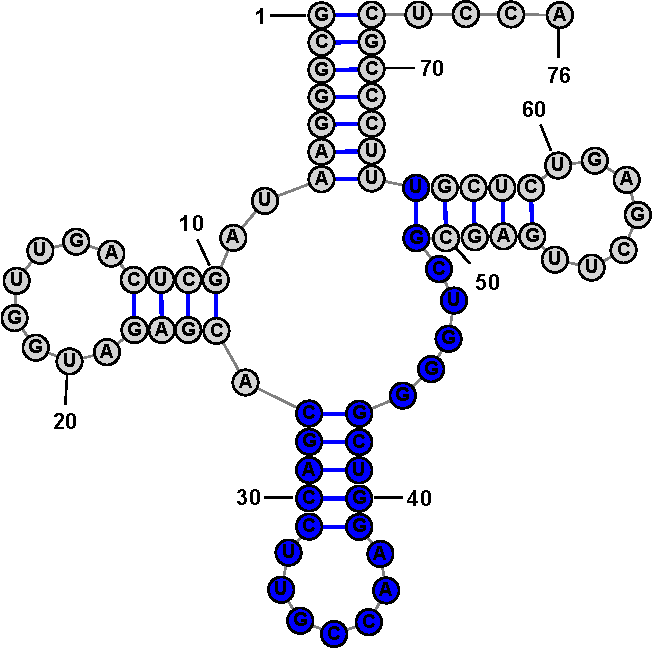
\includegraphics[scale=0.3]{figs/gold_RNAstructure}
% &
% 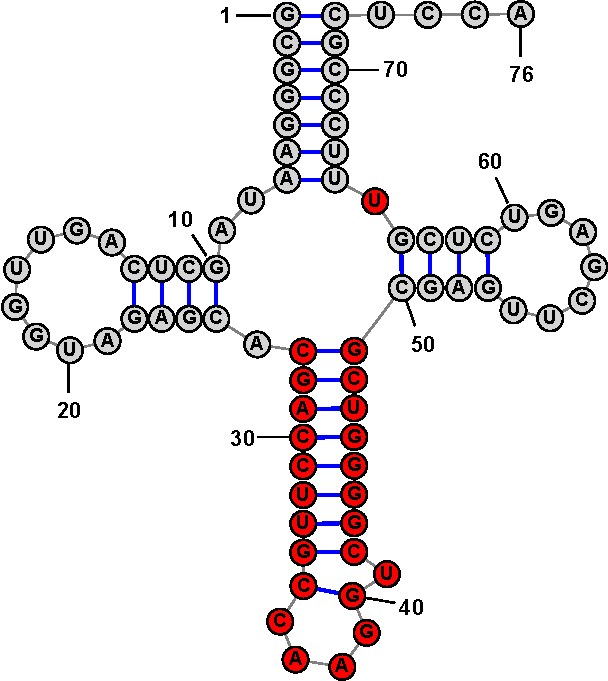
\includegraphics[scale=0.3]{figs/mfe_RNAstructure}\\
% \hspace{-3cm}\panel{C} & \hspace{-3cm}\panel{D}\\[-0.4cm]
% 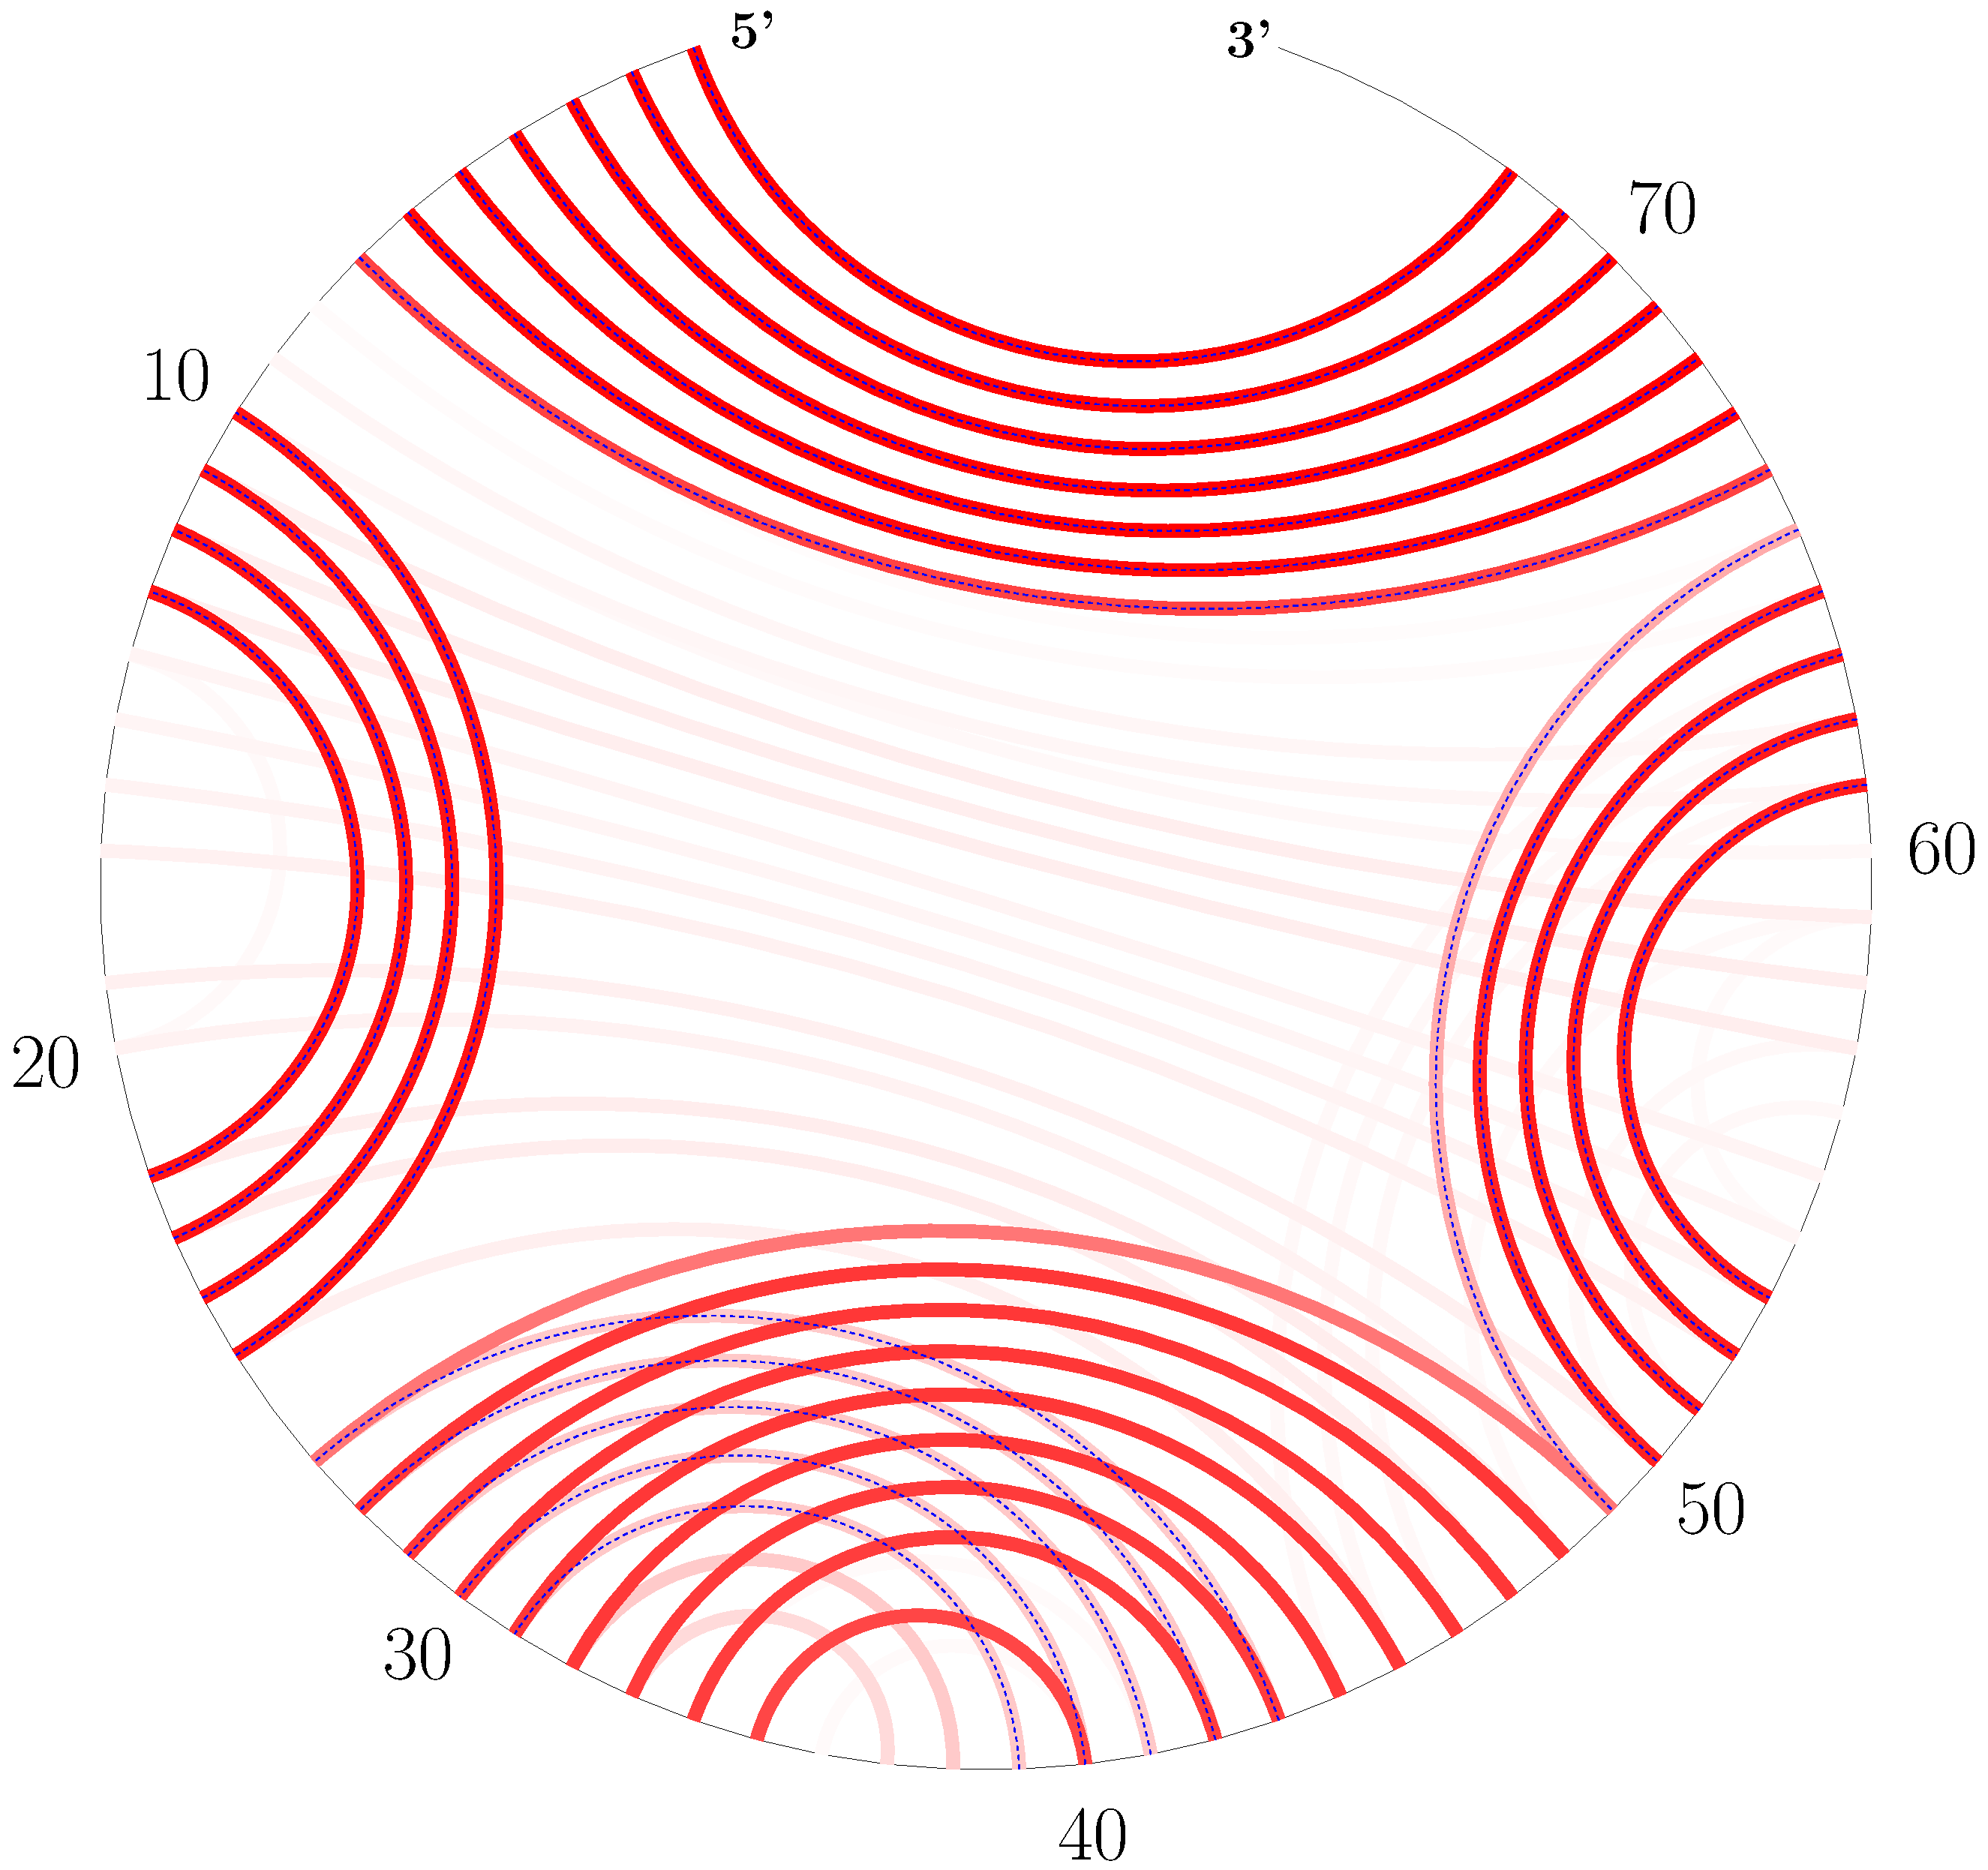
\includegraphics[scale=0.085]{figs/tRNA_circular}
% &
% 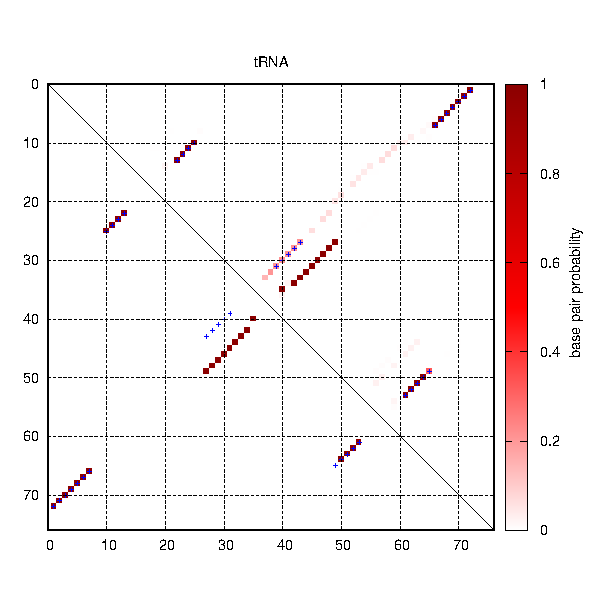
\includegraphics[scale=0.4]{figs/tRNA_heatmap_dark}

% \end{tabular}
% \caption{
% Comparison of MFE-based method and partition function-based method. 
%     {\bf A}: ground truth secondary structure of {\it E.~coli} tRNA$^\textit{Gly}$; 
%     {\bf B}: the corresponding MFE structure. 
%     Structural difference are denoted with blue in ground truth structure and red in MFE structure;
%     {\bf C}: the corresponding circular representation.
%     Ground truth base pairs are denoted with dash blue lines. 
%     Base pair probabilities are denoted with red solid lines and line shade is proportional to probability value.
%     {\bf D}: the corresponding heatmap representation.
%     MFE structure (lower triangle) misses some ground truth base pairs (blue cross), 
%     while base pairing probability matrix (upper triangle) covers these correct base pairs. 
% \label{tRNA}}
% \end{figure}


% For past decades, our understanding of ribonucleic acid (RNA) is changing. 
% New proofs reveal that 
% noncoding 
% RNAs %(ncRNAs) 
% Ribonucleic acids (RNAs)
RNAs
are involved in multiple processes, 
such as catalyzing reactions or guiding RNA modifications~\cite{Eddy:2001,Doudna+Cech:2002,Bachellerie+:2002}, 
% and regulating a particular disease~\cite{Kung+:2013},
and their functionalities are highly related to structures.
% but determining the structure using experimental methods is costly and time-comsuming. 
%%%%%%%%5
% from proposal
% Therefore, being able to %rapidly 
% determine the structure is %extremely 
% useful and desired.
% given the overwhelming pace of increase in genomic data (about 1021 base-pairs per year \cite{stephens+:2015}) %[97] 
% and given the small percentage of sequences that have experimentally determined structure. 
% While experimental assays still constitute the most reliable way to determine structures, they are prohibitively costly, slow, and difficult.
However, 
% both 
structure determination techniques, such as X-ray crystallography~\cite{Zhang+Adrian:2014}, 
Nuclear Magnetic Resonance (NMR)~\cite{Zhang+Keane:2019}, 
and 
% chemical probing methods 
cryo-electron microscopy~\cite{Lyumkis:2019}, 
% ~\cite{Ziehler+Engelke:2001},
though reliable and accurate,
are extremely slow and costly.
% considering the exponentially increasing genomic data (about $10^{21}$ base-pairs per year \cite{stephens+:2015}) 
% and undetermined structures.
% and therefore computational prediction provides an attractive alternative.
%%%%%%%%%%%%
% Due to such limitations, fast and accurate RNA structure prediction is required and desired,
% Due to such limitations, 
% for many RNA tasks 
Therefore,
fast and accurate computational prediction of RNA structure is useful and desired. %required. 
Considering full RNA %tertiary 
structure prediction is challenging~\cite{Miao+:2017},
% \cite{mccaskill:1990},
% even more difficult than protein folding \cite{mccaskill:1990},
% as an alternative
many studies focus on predicting secondary structure,
% the double helices folding structure formed by self-complementary nucleotides
the set of canonical base pairs in the structure 
(A-U, G-C, G-U base pairs)~\cite{Tinoco+Bustamante:1999},
% RNA secondary structure prediction
as it is well-defined, 
% in mathematics formation, 
and provides detailed information to help understand 
% RNA's mechanism of functionality,
the structure-function relationship, and
% functionality 
% as well as further 
%The secondary structure additionally
is a basis to predict full tertiary structure~\cite{Flores+Altman:2010,Seetin+Mathews:2011}.

\begin{figure}%[t]
%  \center
  \vspace{-0.5cm}
\begin{tabular}{ccc}
% \hspace{-3cm}\panel{A} & \\[-0.6cm]
% % \\[-0.6cm]
  % \multicolumn{2}{c}{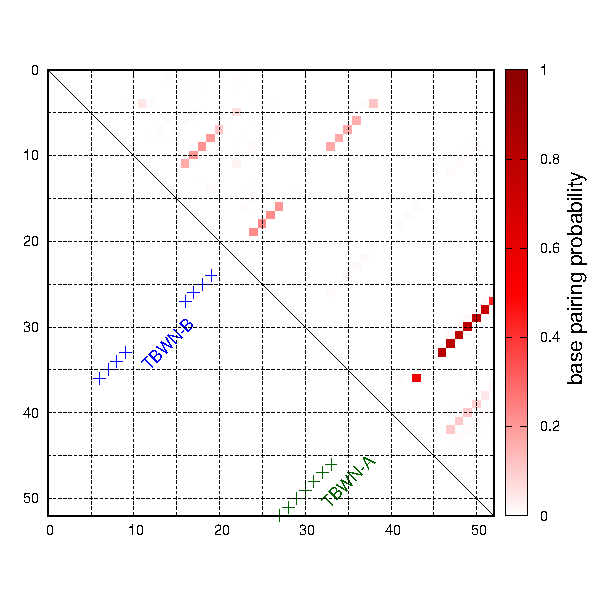
\includegraphics[scale=0.7]{figs/heatmap_fig1A}}
  \\[-0.1cm]  
  \hspace{-.3cm}
  \raisebox{1.7cm}{\panel{A}}
  \hspace{-.3cm}
  %\hspace{-3.5cm}
  \raisebox{-1.cm}{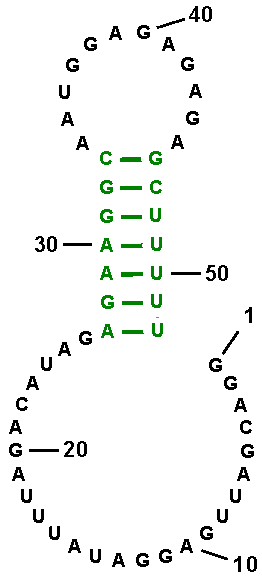
\includegraphics[scale=0.3]{figs/TBWN-A-3}}
  &
  \hspace{.0cm}\raisebox{.8cm}{\panel{B}}
\raisebox{-2.2cm}{\hspace{-.7cm}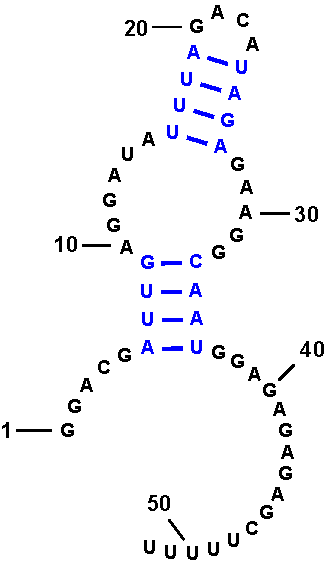
\includegraphics[scale=0.3]{figs/TBWN-B-4}}
&
  %\hspace{-0.5cm}
\hspace{-0.3cm}\raisebox{2.cm}{\mtwo{{\raisebox{4.5cm}{\panel{C}} \hspace{-0.3cm} 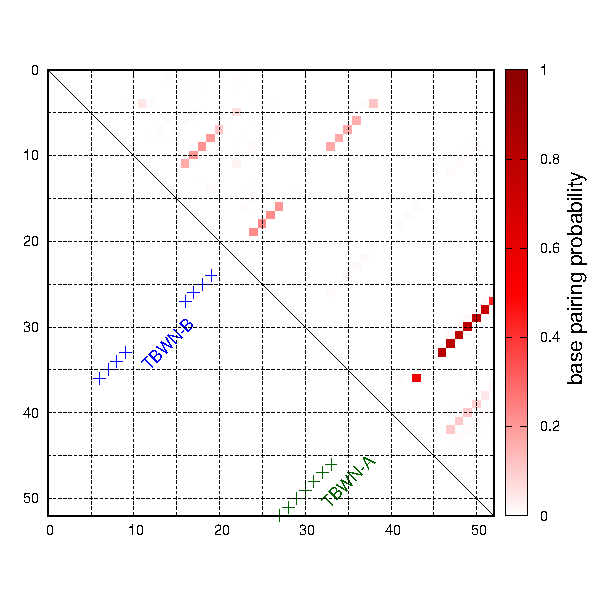
\includegraphics[scale=0.5]{figs/heatmap_fig1A}}}}
\\[0.2cm]
%\hspace{-1cm}
% 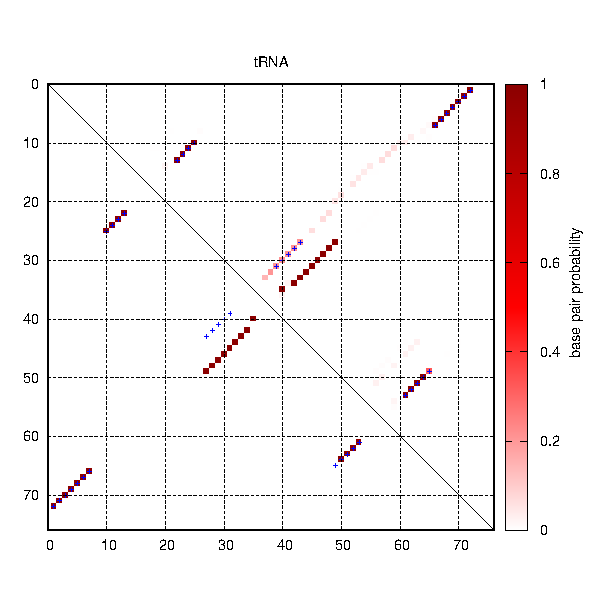
\includegraphics[scale=0.4]{figs/tRNA_heatmap_dark}
\end{tabular}
\\[0.2cm]
\panel{D}
\\[-0.2cm]
%\centering
  \begin{tabular}{@{}c@{ }|@{}c@{ }|l@{\!}c@{ }|l@{\!}c@{}}
    & \ span & \multicolumn{2}{c|}{minimum free energy} & \multicolumn{2}{c}{partition-function} \\
    \hline
    bottom-up, {\em exact} &$\infty$ &    Zuker\cite{zuker+stiegler:1981} & $O(n^3)$ & McCaskill\cite{mccaskill:1990} & $O(n^3)$ \\    
    \hline
    \mtwo{local folding} & \mtwo{$L$}  &  \mtwo{Localfold\cite{lange+:2012}} & \mtwo{$O(nL^2)$} & {RNAplfold\cite{bernhart+:2006}} & \mtwo{$O(nL^2)$}\\
                  &           &   &       &   Rfold\cite{kiryu+:2008}        &\\
    \hline    
    left-to-right, {\em exact}  & \mtwo{$\infty$} & \mtwo{\linearfold\cite{huang+:2019}} & $O(n^3)$  & \mtwo{\linearpartition} & $O(n^3)$\\
     \quad + {\em beam pruning} &     && $O(n b\log b)$ && $O(n b^2)$
    %% left-to-right & \mtwo{\linearfold, $O(n b\log b)$} & \linearpartition, $O(n b^2)$\\[-0.1cm]
    %% + {\em beam pruning} & 
  \end{tabular}
  %% \caption{Comparison between classical, local, and left-to-right algorithms for MFE and partition function calculation. 
  %%   \linearfold and \linearpartition enjoy linear runtime thanks to left-to-right order which enables heuristic beam pruning,
  %%   and both become exact $O(n^3)$ algorithms without pruning. % size $b$ is $+\infty$.
  %%   ``Span'' denotes the maximum pair distance allowed ($\infty$ means no limit);
  %%   it is a small constant in local methods (e.g., default $L$=70 in RNAplfold).
  %%   \label{tab:overall}
  %% } 
\caption{
  %An example % of Tebowned RNA
%  illustrates 
% some RNAs 
  %that
  An RNA can fold into multiple structures at equilibrium.
  {\bf A--B}:~Two 
  %such 
  secondary structures of Tebowned RNA: TBWN-A and TBWN-B~\cite{Cordero+Das:2015}.
{\bf C}: upper triangle shows the estimated base pairing probability matrix for this RNA using \viennarnafold,
where darker red squares represent higher probility base pairs;
the lower triangle shows the two different structures; %TBWN-A and TBWN-B  %(in green)  (in blue),
%at equilibrium;
%(green crosses for TBWN-A and blue for TBWN-B base pairs);
    %    {\bf C}: TBWN-B secondary structure.
{\bf D:} Comparison between classical, local, and left-to-right algorithms for MFE and partition function calculation. 
    \linearfold and \linearpartition enjoy linear runtime because of a left-to-right order that  enables heuristic beam pruning,
    and both become exact $O(n^3)$ algorithms without pruning. % size $b$ is $+\infty$.
    ``Span'' denotes the maximum pair distance allowed ($\infty$ means no limit);
    it is a small constant in local methods (e.g., default $L$=70 \nts in RNAplfold).
\label{fig:overview}}
\vspace{-0.3cm}
\end{figure}




% Secondary structure prediction problem, 
% though still difficult, 
% is well-defined in mathematics formation, and can be suitable modeled with the decomposable substructures. 
% Utilizing this decomposable nature, 
RNA secondary structure prediction is NP-complete~\cite{Pedersen+:2000},
but nested (i.e., pseudoknot-free) secondary structures can be predicted with
cubic-time dynamic programming algorithms. 
% based on an important paradigm free energy minimization 
Commonly, the minimum free energy (MFE) 
structure is predicted~\cite{nussinov+jacobson:1980, zuker+stiegler:1981}.
% when a single structure is expected.
% and some prediction systems based on these algorithms, such as RNAstructure \cite{mathews+turner:2006}, \contrafold \cite{do+:2006} and \viennarnafold \cite{lorenz+:2011}, 
% have greatly improved the accuracy of prediction and are widely used.
% MEA -> partition function 
% For a given sequence, predicting the structure of minimum free energy (MFE) under certain free energy model by dynamic programming is a classical method for RNA secondary structure prediction. 
% cted.Free energy minimization is an important paradigm for predicting structure when a single structure is expe
% In the absence of many homologous sequences, the accuracy of MFE structure is 73\% in average \cite{mathews:2004}.
% However, this method assumes all thermodynamic parameters are correct and the energy model is perfect, which are both no the case in reality.
% Also, this method neglects the facts that multiple conformations exits at equilibrium \cite{mathews:2004}.
% This method 
% MFE method gives a practical solution to predict a single secondary structure, 
At equilibrium, the MFE structure is the most populated structure, 
but it 
% it neglects the fact that 
is a simplification because 
multiple conformations exist 
% at equilibrium 
as an equilibrium ensemble 
for one RNA sequence~\cite{mathews:2004}.
For example, many mRNAs {\textit {in vivo}} form a dynamic equilibrium 
and fold into a population of structures~\cite{Long+:2007, Lu+:2008, Tafer+:2008, lai+:2018}; 
% as well as abandons all pseudoknotted structures.
% Many RNA sequences, for example mRNAs, exist in a thermodynamic ensemble of structures 
% \cite{lai+:2018}.%[53].
% As an alternative, partition function-based method \cite{mccaskill:1990} provides an ensemble of all pseudoknot-free structures, and based on it base pairing probabilities and structural entropy \cite{Huynen+} can be calculated.  
% As an alternative, 
Figure~\ref{fig:overview}A--B shows the example of Tebowned RNA
which folds into more than one structure at equilibrium.
% ~\cite{Cordero+Das:2015}.
% TBWN-A, which has a long helices at 3'-end, 
% is the majority structure and accounts for $56 \pm 16\%$ of ensemble.
% While TBWN-B, which has two short helices at 5'-end, takes up $27 \pm 12\%$ of ensemble.
% Besides TBWN-A and TBWN-B illustrated in Figure~\ref{fig:overview}, Tebowned RNA can also fold into the state of TBWN-C 
% with a smaller ensemble proportion of $17 \pm 11\%$.
In this case, the prediction of one single structure, such as the MFE structure, 
is not expressive enough to capture multiple states of RNA sequences %Tebowned RNA %folding.
at equilibrium.

% Rather than predicting one single stucture, 
% partition function-based methods estimate the folding in a different point of view by
% taking into account ensemble of structures at equilibrium with Boltzmann Distribution.  
% Partition function, the sum of equilibrium constants for all possible secondary structures,
% is the normalization terms for calculating given secondary structure in the boltzmann ensemble.
Alternatively, we can compute the partition function, 
which is the sum of the equilibrium constants for all possible secondary structures,
and is the normalization term for calculating the probability of a secondary structure in the Boltzmann ensemble.
% Starting from the partition function,
% these methods are able to model mix of conformations,
% and further 
% we can % also
The partition function calculation can also be used to 
calculate base pairing probabilities of each nucleotide $i$ 
paired with each of possible nucleotides $j$~\cite{mccaskill:1990, mathews:2004}. 
% Base pairs with high probabilities 
% %in the matrix 
% indicate strong confidence of pairing in prediction,
% and are more likely to be paired in ground truth structures
% \cite{mathews:2004, Zuber+:2018}. 
% Figure~\ref{fig:overview}A 
In Figure~\ref{fig:overview}C,
the upper triangle presents the base pairing probability matrix of Tebowned RNA using \viennarnafold, 
showing that base pairs in TBWN-A have higher probabilities (in darker red) than
base pairs in TBWN-B (in lighter red).
This is consistent with the experimental result, i.e.,
TBWN-A is the majority structure that accounts for $56 \pm 16\%$ of the ensemble, 
while TBWN-B takes up $27 \pm 12\%$~\cite{Cordero+Das:2015}. % of the ensemble

% ~\cite{Cordero+Das:2015}.
% Besides producing base pairing probability matrix, 

%% \begin{table}
%% %  \vspace{-0.5cm}
%%   \centering
%%   \begin{tabular}{@{}c@{ }|@{}c@{ }|l@{\!}c@{ }|l@{\!}c@{}}
%%     & span & \multicolumn{2}{c|}{minimum free energy} & \multicolumn{2}{c}{partition-function} \\
%%     \hline
%%     bottom-up, {\em exact} &$\infty$ &    Zuker\cite{zuker+stiegler:1981} & $O(n^3)$ & McCaskill\cite{mccaskill:1990} & $O(n^3)$ \\    
%%     \hline
%%     \mtwo{local folding} & \mtwo{$L$}  &  \mtwo{Localfold\cite{lange+:2012}} & \mtwo{$O(nL^2)$} & {RNAplfold\cite{bernhart+:2006}} & \mtwo{$O(nL^2)$}\\
%%                   &           &   &       &   Rfold\cite{kiryu+:2008}        &\\
%%     \hline    
%%     left-to-right, {\em exact}  & \mtwo{$\infty$} & \mtwo{\linearfold\cite{huang+:2019}} & $O(n^3)$  & \mtwo{\linearpartition} & $O(n^3)$\\
%%      \quad + {\em beam pruning} &     && $O(n b\log b)$ && $O(n b^2)$
%%     %% left-to-right & \mtwo{\linearfold, $O(n b\log b)$} & \linearpartition, $O(n b^2)$\\[-0.1cm]
%%     %% + {\em beam pruning} & 
%%   \end{tabular}
%%   \caption{Comparison between classical, local, and left-to-right algorithms for MFE and partition function calculation. 
%%     \linearfold and \linearpartition enjoy linear runtime thanks to left-to-right order which enables heuristic beam pruning,
%%     and both become exact $O(n^3)$ algorithms without pruning. % size $b$ is $+\infty$.
%%     ``Span'' denotes the maximum pair distance allowed ($\infty$ means no limit);
%%     it is a small constant in local methods (e.g., default $L$=70 in RNAplfold).
%%     \label{tab:overall}
%%   } 

%% \end{table}


% !TEX root = main.tex
\begin{figure}[t]
\vspace{-0.9cm}
\center
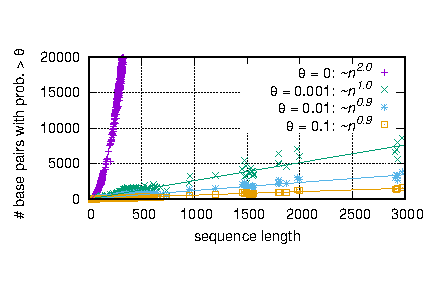
\includegraphics[width=.42\textwidth]{figs/Vienna_RNAfold_num_pij_curves.pdf}\\[-1cm]
\caption{
  Although the total number of possible base pairings scales $O(n^2)$ with the sequence length $n$
  (using the probability matrix from \viennarnafold as an example),
  with any reasonable threshold $\theta$, the number of surviving pairings (in colors for different $\theta$) grows linearly,
  suggesting our approximation, only computing $O(n)$ pairings, is reasonable.
  \label{fig:linearpairs}}
\vspace{-0.7cm}
\end{figure}


In addition to model multiple states at equilibrium, 
base pairing probabilities are used for downstream prediction methods, 
such as maximum expected accuracy (MEA)~\cite{Knudsen+Hein:2003, do+:2006}, 
to assemble a structure with improved accuracy compared with the MFE structure~\cite{lu+:2009}.
% As a by-product, the pair probabilities also enable maximum expected accuracy (MEA) structure prediction 
% \cite{do+:2006, lu+:2009}. % [29, 62].
Other downstream prediction methods, 
such as 
% HotKnot \cite{Ren+:2005}, % not based on partition function
ProbKnot~\cite{bellaousov+mathews:2010}, 
ThreshKnot~\cite{Zhang+:2019},
DotKnot~\cite{Sperschneider+Datta:2010} 
and IPknot~\cite{sato+:2011},
use base pairing probabilities to predict pseudoknotted structures with heuristics,
which is beyond the scope of standard cubic-time algorithms.
Additionally, the partition function 
% can also be applied to do stochastic sampling based on the ensemble distribution
is the basis of stochastic sampling, 
in which structures are sampled with their probability of occurring 
in the Boltzmann ensemble~\cite{Ding+Lawrence:2003, mathews:2006}.

% Moreover, although partition function-based method excluded pseudoknotted structures during dynamic programming process, 
% it is able to predict pseudoknotted base pairs and structure by using pair probability matrix, and pseudoknotted prediction systems such as HotKnot \cite{Ren+:2005}, ProbKnot \cite{bellaousov+mathews:2010}, DotKnot \cite{Sperschneider+Datta:2010} and IPknot \cite{Sato+:2011} all take pair probability matrix as inputs. 
% Figure~\ref{tRNA} compares MFE-based and partition function-based methods.
% Furthermore, single structure prediction based on partition function calculation, such as maximum expected accuracy (MEA) ThreshKnot \cite{do+:2006, threshknot}, achieves higher accuracy in average. 


% speed
Therefore, there has been a shift from the classical MFE-based methods to partition function-based ones.
These latter methods, 
as well as the prediction engines based on them, such as partition function-mode of RNAstructure~\cite{mathews+turner:2006}, 
\viennarnafold~\cite{lorenz+:2011}, 
and \contrafold~\cite{do+:2006},
are all based on the seminal algorithm that McCaskill pioneered~\cite{mccaskill:1990}.
It employs a dynamic program to capture all possible (exponentially many) nested structures,
but its $O(n^3)$ runtime still scales poorly for longer sequences. 
This slowness %of partition function-based methods
is even more severe than the $O(n^3)$-time MFE-based ones
%with the same $O(n^3)$ time complexity
due to a much larger constant factor.
For instance, for 
% {\it E.~coli} 
{\it H.~pylori} 23S rRNA (sequence length 2,968~{\it nt}),
\viennarnafold's %(version 2.4.11)
computation of the partition function and base pairing probabilities
is 9$\times$ slower than MFE (71 vs.~8 secs),
%% takes 8 seconds to find the MFE structure, 
%% but %36+37=
%% 71 seconds to compute the partition function
%% %and another 37 seconds for
%% and base pairing probabilities, %, respectively,
%% which is a 9x slowdown;
%it is even worse for
%to make things worse,
and \contrafold % is even slower,
%% which takes about 6 seconds to find the MFE structure, % prediction,
%% but 50+70=120 seconds to compute the partition function and base pairing probabilities, respectively,
%gives a
is even 20$\times$ slower (120 vs.~6~secs).
The slowness %(both $O(n^3)$-time and the constant factor)
prevents their applications to longer sequences.
% 132.248859 contrafold

% , which is more than 9 $\times$ slower. 
% because function-based method takes two-round cubic loops for inside-outside calculation.

To address this $O(n^3)$-time bottleneck, %alleviate the cubic-factor slowness, 
we present \linearpartition, 
which is inspired by our %efficient linearization idea of \linearfold \cite{huang+:2019}
recently proposed \linearfold algorithm~\cite{huang+:2019} 
that approximates the MFE structure in linear time.
Using the same idea, \linearpartition can approximate
the partition function and base pairing probability matrix in linear time.
% Recently, \linearfold \cite{huang+:2019} 
% presents the first linear-time and linear-space MFE-based RNA folding prediction system.
% For the same 
% % {\it E.~coli} 
% {\it H.~pylori} 23S rRNA, \linearfold spends about 2 seconds, leading to a 4$\times$ runtime decrease.
% % Overall, \linearfold achieves significant efficiency and scalability improvement and higher accuracy. 
% % the first linear-time MFE-based (approximate) algorithm for RNA folding, 
% % achieves significant efficiency and scalability improvement and higher accuracy 
% % than classical $O(n^3)$ MFE-based method, especially on long sequences. 
% Inspired by the efficient linearization idea of \linearfold, we present \linearpartition, 
% which can approximate the partition function and base pairing probability matrix in linear time, 
% addressing speed bottleneck in existing systems.
% Similar as \linearfold, 
Like \linearfold,
\linearpartition % incrementally 
scans the RNA sequence from 5'-to-3'
using a left-to-right dynamic program that runs in $O(n^3)$ time,
but unlike the classical bottom-up McCaskill algorithm~\cite{mccaskill:1990} with the same speed,
our left-to-right scanning makes it possible to apply the beam pruning heuristic~\cite{Huang+Sagae:2010} 
%to narrow down the search space, 
to achieve linear runtime in practice; see Fig~\ref{fig:overview}D.
 % with substructure of lower energy.
% and only retain states with top $b$ free energy of ensemble (inside score), 
% where $b$ is the beam size.
% Though introducing beam prune to filter some structures,
Although the search is approximate,
the well-designed heuristic ensures 
%that only states with worse ensemble free energy
the surviving structures capture the bulk of the free energy of the ensemble.
It is important to note that, unlike local folding methods in Fig.~\ref{fig:overview}D,
our algorithm does {\em not} impose any limit on the base-pairing distance;
in other words, it is a {\em global} partition function algorithm.
%and the resulting partition function is close to the exact version.

%  (inside score) 
% are pruned,
% and partition function is still similar as optimal algorithm.
% and the majority is catched.

More interestingly, as Figure~\ref{fig:linearpairs} shows,
even with the $O(n^3)$-time McCaskill algorithm, %(like the one implemented in \viennarnafold),
the resulting number of base pairings with reasonable probabilities (e.g., >0.001)
grows only linearly with the sequence length.
This suggests that our algorithm, which only computes $O(n)$ pairings by design,
is a reasonable approximation.

% \linearpartition, inherits efficiency and accuracy of \linearfold. 

% \linearpartition is 11$\times$ faster than \viennarnafold for the longest sequence ({\it H.~pylori} 23S rRNA, 2,968 nucleotides) in the ArchiveII dataset,
% and 256$\times$ faster for the longest sampled sequence (15,780 nucleotides) from RNAcentral that \viennarnafold can run.
\linearpartition is 2,771$\times$ faster than \contrafold for the longest sequence (32,753~{\it nt})
% 32,767 nucleotides) 
that \contrafold can run 
in the dataset (2.5 days vs.~1.3 min.).
% Meanwhile, \linearpartition leads to a small improvement on PPV and Sensitivity compared with \viennarnafold.
% % in both MEA and ThreshKnot prediction 
% % using the probability matrix computed in linear time.
% Surprisingly, \linearpartition achieves higher accuracy improvement on longer families (16S and 23S rRNA).
Interestingly, \linearpartition is orders of magnitude faster {\em without} sacrificing accuracy.
In fact, the resulting base pairing probabilities are even better correlated with ground truth structures,
and 
when applied to downstream structure prediction tasks,
%such as MEA and ThreshKnot (a thresholded version of ProbKnot),
they lead to a small accuracy improvement on longer families (small and large subunit rRNA),
as well as a substantial accuracy improvement on long-distance base pairs (500+ \nts apart).
%% Our work is the first major speedup on this important problem in 30 years, and
%% enables calculations on full length sequences such as mRNAs.
%% has numerous applications
%% such as  sampling.

% \begin{itemize}
% \item Present an alternative left-to-right dynamic programming fashion for partition function calculation.
% \item The first algorithm to achieve linear runtime and space for partition function and base pairing probability calculation.
% % \item . 
% \end{itemize}

% more striking than LinearFold
Although both \linearpartition and \linearfold use linear-time beam search,
the success of the former is arguably more surprising,
since rather than finding one single optimal structure, 
\linearpartition needs to sum up exponentially many structures
that capture the bulk part of the ensemble free energy.
% For users, 
\linearpartition also results in more accurate downstream structure predictions than \linearfold.
%and is able to serve tasks such as pseudoknot prediction and accessibility calculation.





% \label{sec:rnaintro}
% \input{rnaintro}

% \label{sec:linpar}
% \input{linpar}

\label{sec:algorithm}
% !TEX root = main.tex
\vspace{-0.4cm}
\section{The \linearpartition Algorithm}
\vspace{-0.1cm}


\newcommand{\pluseq}{\mathrel{+}=}


We denote $\vecx\!=\!x_1 ... x_n$ as the input RNA sequence of length $n$, and $\mathcal{Y(\vecx)}$ as the set of all possible secondary structures of $\vecx$.  
% $\vecy$ is a secondary structure 
% of $\vecx$ 
% in $\mathcal{Y(\mathbf x)}$. 
The partition function is: % $Q(\vecx)$ 
% of $\vecx$ 
%is then: %defined as:
\begin{equation}
	Q(\vecx)=\sum_{\vecy \in \mathcal{Y(\mathbf x)}} e^{-\frac{\Delta G^{\circ}({\vecy})}{RT}} \notag
\end{equation}
where $\Delta G^{\circ}({\vecy})$ is the  conformational Gibbs free energy change of structure $\vecy$, 
$R$ is the universal gas constant 
and $T$ is the thermodynamic temperature.
$\Delta G^{\circ}({\vecy})$ is calculated using loop-based Turner free-energy model~\cite{mathews+:1999, Mathews+:2004}, 
but for presentation reasons, % simplicity in presenting the algorithm
we use a revised Nussinov-Jacobson energy model, 
i.e., a free energy change of $\delta(\vecx, j)$ for unpaired base at position $j$ 
and a free energy change of $\xi(\vecx, i, j)$ for base pair of $(i,j)$.
For example, we can assign $\delta(\vecx, j)\!=\!1$ kcal/mol and $\xi(\vecx, i, j)\!=\!-3$ kcal/mol for CG pairs and $-2$ kcal/mol for AU and GU pairs. 
Thus, $\Delta G^{\circ}({\vecy})$
can be decomposed as:
\begin{equation}
	\Delta G^{\circ}({\vecy}) = \sum_{j \in \unpaired(\vecy)} \delta(\vecx, j) \ + \sum_{(i,j) \in \pairs(\vecy)} \xi(\vecx, i, j) \notag
\end{equation}
where ${\textrm {unpaired}}(\vecy)$ is the set of unpaired bases in $\vecy$, 
and ${\textrm {paired}}(\vecy)$ is the set of base pairs in $\vecy$.
% and $y_j$ denotes the position $j$ of $\vecy$.
%With the simplified model,
The partition function now decomposes as: % $Q(\vecx)$ is:
\begin{equation}
	Q(\vecx)=\sum_{\vecy \in \mathcal{Y(\vecx)}} (\prod_{j \in \unpaired(\vecy)} e^{-\frac{\delta(\vecx, j)}{RT}} \prod_{(i,j) \in \pairs(\vecy)} e^{-\frac{\xi(\vecx, i, j)}{RT}}) \notag
\end{equation}


%% We provide the pseudocode of our simplified linear-time partition function algorithm (based on the revised Nussinov-Jacobson energy model) in Figure~\ref{fig:algorithm},
%% illustrating how our algorithm linearizes partition function calculation. 

% \linearpartition scans from 5'-end to 3'-end (left-to-right), 
% calculating $Q_{0,j}$, which is the partition function from 5'-end to current step $j$.
%In order to define our algorithm,
We first define {\bf span} $[i,j]$ to be the subsequence $x_i ... x_j$
(thus $[1,n]$ denotes the whole sequence \vecx, and $[j, j\!-\!1]$ denotes the empty span between $x_{j-1}$ and $x_j$ for any $j$ in $1..n$).
We then define a {\bf state} to be a span associated with its partition function:\\[-0.4cm] % $\Qf{i,qj]$: 
\[
  [i,j]: \Qf{i}{j}
\]
%% where $i$ and $j$ are start and end points of the span ($i=0..n, j=1..n$ where $n$ is the sequence length), %is the index of an openning bracket, 
%% % $j$ is the index of current step, 
%% and $\Qf{i,j]$ is the partition function of span $[i,j]$. %state $\langle i,j \rangle$. 
%% % We require each state $\langle i,j \rangle$ only has at most one openning bracket at $i$.
%Each state $\langle i,j \rangle :
where % $\Qf{i}{j}$ 
\begin{center}
  \vspace{-0.6cm}
  $\displaystyle \Qf{i}{j} = \sum_{\vecy \in \mathcal{Y}(x_i ... x_j)} e ^{-\frac{\Delta G^{\circ}(\vecy)}{RT}}$
  \vspace{-0.1cm}
\end{center}
encompasses all possible substructures for span $[i, j]$, % $[i,j]$, i.e
which can be visualized as
%\begin{center}
%  \vspace{-0.5cm}
%    \hspace{1.6cm}
\raisebox{-0.2cm}{
  \hspace{-0.5cm}
    \begin{tabular}{lr@{\quad}} % adjust alignment with j
    \multicolumn{2}{c}{
      ${\myboxmath{\ \ \Qf{i}{j} \ \ }}$
    }
    \\
    $i$ & $j$
\end{tabular}}
.
%    \end{center}

%which can be visualized as
%\begin{center}
 % \end{center}

%% We require these substructures to have an open bracket at nucleotide $i$.
%% For example, ``\bml\md\md'' and ``\bml\bml\bmr'' 
%% % ``\md\md\md'' 
%% are valid states, 
%% while ``\bml\bml\md'' and ``\md\bml\md'' are invalid.
%% As special cases, states with $i=0$ can have none open brackets to 
%% allow unpaired substructures in 5'-end,
%% i.e., ``\md\md\md'' and ``\md\bml\bmr'' are valid for states $\langle 0,j \rangle : Q(0,j)$.

  \algrenewcommand\algorithmicindent{0.5em}%
  \algnewcommand\algorithmicforeach{\textbf{for each}}
\algdef{S}[FOR]{ForEach}[1]{\algorithmicforeach\ #1\ \algorithmicdo}
\begin{figure}[t]%[b]
% \begin{algorithm}[H]
% \algsetup{linenosize=\tiny}
  % \scriptsize
  % \newcommand{\pluseq}{\mathrel{+}=}
\center
\footnotesize
% \hspace{-0.23cm}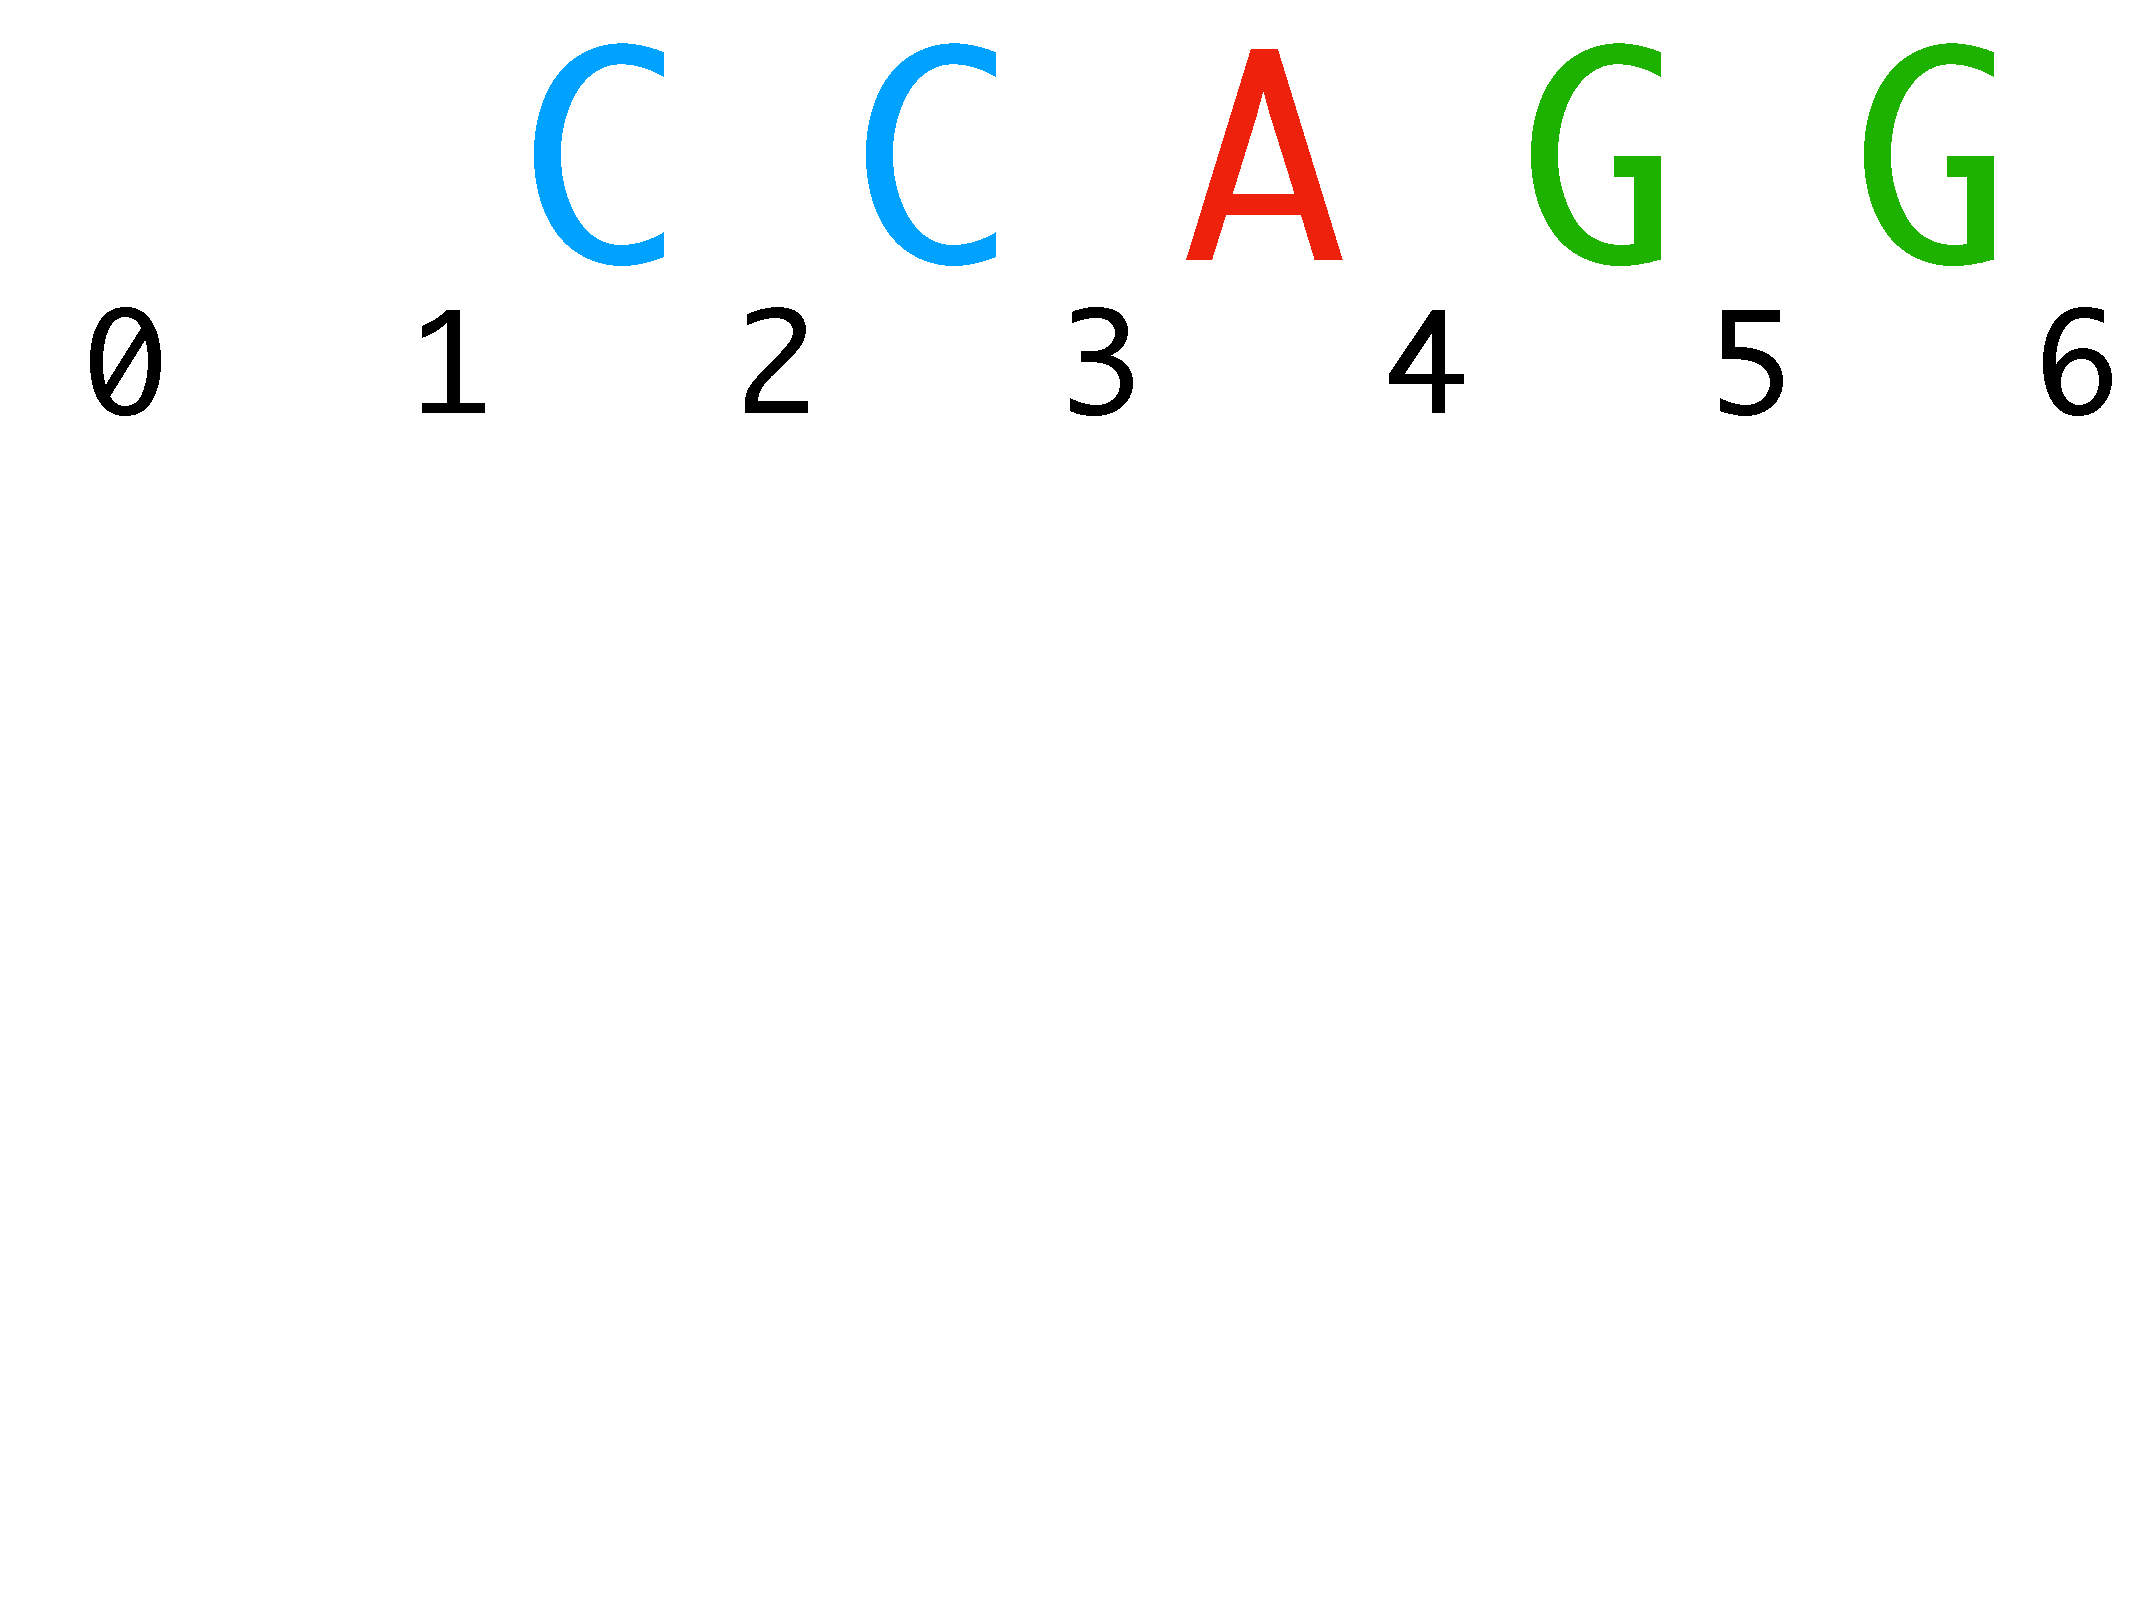
\includegraphics[scale=.16]{figs/index} \\[-3.cm]
%\hspace{-0.23cm}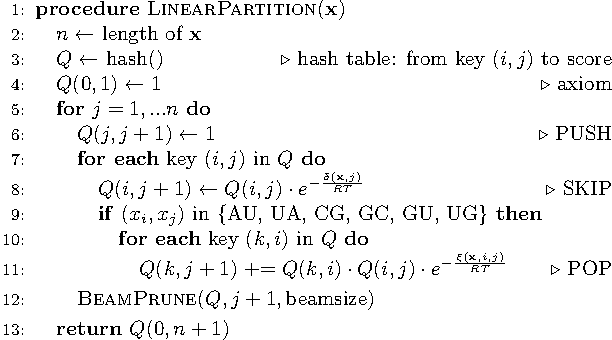
\includegraphics[scale=.83]{figs/algorithm} \\[0.2cm]
\begin{algorithmic}[1]
  \newcommand{\INDSTATE}[1][1]{\State\hspace{#1\algorithmicindent}}
  \setstretch{1.05} % lhuang: usepackage setspace
\Function{LinearPartition}{$\vecx, b$} \Comment{$b$ is the beam size}
% \bindent
    \State $n \gets$ length of $\mathbf x$
    \State $Q \gets$ hash() \Comment{hash table: from span $[i,j]$ to $\Qf{i}{j}$}
    \State $\Qf{j}{j-1} \gets 1$ for all $j$ in $1...n$ \Comment{base cases} \label{line:base}
    \For{$j=1 ... n$}
    \ForEach {$i$ such that $[i,\,j-1]$ in $Q$} \Comment{$O(b)$ iterations}
        \smallskip 
            \State $\Qf{i}{j} \pluseq \Qf{i}{j-1} \cdot e^{-\frac{\delta(\vecx,j)}{RT}} $ \Comment{\nskip} \label{line:skip}
            \If{$x_{i-1}x_j$ in \{AU, UA, CG, GC, GU, UG\}}  \label{line:pair}
                % \State $Q_{i,\,j+1} \gets  C(i,\,j) \cdot e^{-\frac{\xi(\vecx,i,\,j)}{RT}} $
                \ForEach{$k$ such that $[k,\,i-2]$ in $Q$} \Comment{$O(b)$ iters} \smallskip 
                    \State $\Qf{k}{j} \pluseq {\Qf{k}{i-2} \cdot \Qf{i}{j-1} \cdot e^{-\frac{\xi(\vecx,i-1,j)}{RT}}} $ \Comment{\pop} \label{line:pop}
                    % \State $C(0,j+1) \pluseq {C(0,k) \cdot C(k,j+1) \cdot e^{-\frac{\xi(\vecx,i,\,j)}{RT}}} $
                \EndFor
                % \State $C(0,j+1) \pluseq C(0,i) \cdot Q_{i,j+1}$ \Comment{COMBINE}
            \EndIf
        \EndFor
        \State $\textsc {BeamPrune}(Q,j, b)$ \Comment{choose top $b$ out of $Q(\cdot,j)$} \label{line:beamprune}%{see Fig.~\ref{fig:beam_prune_alg}}
        \EndFor
        \vspace{-0.1cm}
    \State \Return $Q$ \Comment{partition function $Q(\vecx)=\Qf{1}{n}$}
% \eindent
\EndFunction
\end{algorithmic}
% \end{algorithm}
\caption{
Partition function calculation pseudocode of a simplified version of the \linearpartition %linear-time partition function calculation
algorithm (the inside phase).
See Fig.~\ref{fig:beam_prune_alg} for the pseudocode of beam pruning (line~\ref{line:beamprune}).
The base-pairing probabilities are computed with the combination of the outside phase
(Fig.~\ref{fig:outside}).
% as well as a beam prune algorithm. 
% Here we model hash tables following Python dictionaries, where $(i, j) \in C$ checks whether the key $(i, j)$ is in the hash $C$; 
% this is needed to ensure linear runtime. 
% Quick select algotithm is used in beam prune, 
% and we skip the details for quick select here since it is well known.
% Real \linearpartition system is much more involved, but the pseudocode illustrates the left-to-right partition function calculation idea using a Nussinov-like fashion.
The actual algorithm using the Turner model is available on \href{https://github.com/LinearFold/LinearPartition}{GitHub}.
%See Fig.~\ref{fig:beam_prune_alg} for {\sc BEAMPRUNE} function.
\label{fig:algorithm}}
\vspace{-.3cm}
% \end{figure*}
\end{figure}


For simplicity of presentation,
in the pseudocode in Fig.~\ref{fig:algorithm}, $Q$ is notated as a hash table,
mapping from  $[i,j]$ to %its partition function
$\Qf{i}{j}$;
see Supplementary Information Section~\ref{sec:si:algdetails} for details
of its efficient implementation. % to make sure the overall runtime is $O(nb^2)$.
As the base case, we set $\Qf{j}{j-1}$ to be 1 for all $j$,
meaning all empty spans have partition function of 1 (line~\ref{line:base}).
%% %to store and look up states.   
%% $\langle 0,1 \rangle:1.0$ represents the dummy head state, 
%% whose partition function $Q(0,1)$ is initialized with value $1$.
%% This represents a structure with no pairs, 
%% i.e., the random coil, 
%% which is the reference state (free energy change of 0) and thus has equilibrium constant of 1.
%% {\color{blue}?????? (added by Mathews, but state <0,1>:1 is a singleton not a coil)}
Our algorithm then scans the sequence from left-to-right (i.e., from 5'-to-3'),
and at each nucleotide $x_j$ ($j=1...n$), % (the length of the sequence), 
% state $\langle 0,j+1 \rangle$ can always be extended with ``\md'' from state $\langle 0,j \rangle$.
% with its 
% Then we define three actions, PUSH, SKIP and POP
% to search states $\langle \cdot,j+1 \rangle$:
we perform two actions: %, \nskip and \pop:
%three actions, PUSH, SKIP and POP, are performed:
% similar as in \linearfold but different 
\begin{itemize}
%% \item PUSH: create a new state $\langle j,j \rangle:1$ representing an open bracket at $j$,
%% whose partition function is 1. 

%% 	% \begin{equation*}
%% 	% 	\frac{\langle i,j \rangle : \Qf{i,j]}{\langle j,j+1 \rangle : 1.0}
%% 	% \end{equation*}

\item \nskip (line~\ref{line:skip}): We extend each %state $[i,\,j-1]: \Qf{i,\,j-1]$ to a new state $[i,j]: \Qf{i,j]$
span $[i,\,j\!-\!1]$ in $Q$ to $[i,j]$ %: \Qf{i,j]$
by adding an unpaired base $y_j\!=$``\md'' (in the dot-bracket notation) to the right of each substructure in $\Qf{i}{j-1}$,
updating $\Qf{i}{j}$: % as follows:
\[
\Qf{i}{j} \pluseq \Qf{i}{j-1} \cdot e^{-\frac{\delta(\vecx, j)}{RT}}
\]
which can be visualized as
%\begin{center}
%  \vspace{-0.7cm}
%  \qquad \qquad
  \begin{tabular}{lr@{\,\quad}} % adjust alignment with j
    \multicolumn{2}{c}{
      $\overbrace{\myboxmath{\ \ \Qf{i}{j-1} \ \ } \ \Huge\md\!\!\!\!}^{\Qf{i}{j}}$
    }
    \\
    $i$ & $j$
  \end{tabular}.
%\end{center}
%% \begin{center}
%%   {

%%     \begin{tabular}{@{}l@{\;}c@{}}
%%       %      \hline
%%       \multicolumn{2}{c}{$\Qf{i,j]$}\\[0.1cm]
%%       \hline
%%   \myboxmath{\quad \Qf{i,j-1]\quad} & {\large\md} \\
%% %  \hline
%%    \multicolumn{1}{l}{$i$} & $j$
%%     \end{tabular}
%% }
%% \end{center}



	% \begin{equation*}
	% 	\frac{\langle i,j \rangle : \Qf{i,j]}{\langle i,j+1 \rangle : \Qf{i,j] \cdot e^{-\frac{\delta(\vecx, j)}{RT}}}
	% \end{equation*}
\vspace{-0.2cm}
\item \pop (lines~\ref{line:pair}--\ref{line:pop}): If $x_{i-1}$ and $x_j$ are pairable,
we combine span $[i,j-1]$ in $Q$ %[i,j]$ 
with each combinable ``left'' span $[k,i-2]$ in $Q$ %: \Qf{k,i-1]$,
% and create a new state $\langle k,j \rangle:Q(k,j)$,
% where $Q(k,j+1)=Q(k,i) \cdot \Qf{i,j] \cdot e^{-\frac{\xi(\vecx, i, j)}{RT}}$.
and update the resulting span $[k,j]$'s partition function % $[k,j+1]: Q(k,j+1)$
%as follows: 
\[
\Qf{k}{j} \pluseq \Qf{k}{i-2} \cdot \Qf{i}{j-1} \cdot e^{-\frac{\xi(\vecx, i-1, j)}{RT}}.
\]
This means that every substructure in $\Qf{i}{j-1}$ can be combined
with every substructure in $\Qf{k}{i-2}$ and a base pair $(i-1, j)$
to form one possible substructure in $\Qf{k}{j}$:
\begin{center}
  \vspace{-0.4cm}
  \begin{tabular}{l@{}r@{}l@{}r@{\,\quad}} %adjust alignment with j
    \multicolumn{4}{c}      
                {$\overbrace{\myboxmath{\; \Qf{k}{i-2}\; } {\Large\ml} \;\; \myboxmath{\; \Qf{i}{j-1}\; } \; {\Large\mr}}^{\Qf{k}{j}}$} \\
  $k$ \hspace{1.15cm} & $i\!-\!1$ & \hspace{0.02cm} {$i$} &  $j$
\end{tabular}
\end{center}
%% \begin{center}
%% \begin{tabular}{l@{}c@{\;}l@{\;}c}
%%   {\myboxmath{\; \Qf{k,i-1]\; }} & \ml & \myboxmath{\quad \Qf{i,j]\quad} & \mr \\
%%   {$x_k$} & $x_{i-1}$ & {$x_i$} & $x_j$
%% \end{tabular}
%% \end{center}

	% \begin{equation*}
	% 	\frac{\langle k,i \rangle : Q(k,i) \ \ \ \ \ \langle i,j \rangle : \Qf{i,j]}{\langle k,j+1 \rangle : Q(k,i) \cdot \Qf{i,j] \cdot e^{-\frac{\xi(\vecx, i, j)}{RT}}}
	% \end{equation*}

% Note that the operator of updating $Q(k,j+1)$ is "+=" (see Figure~\ref{algorithm} line 11).

% \item COMBINE: for each close state $\langle i,j \rangle$, it can be combined with its prefix state $\langle 0,i \rangle$ and form state $\langle 0,j+1 \rangle$:
% 	\begin{equation*}
% 		\frac{\langle 0,i \rangle : Q_{0,i} \ \ \langle i,j \rangle : Q_{i,j}}{\langle 0,j+1 \rangle : Q_{0,i} \cdot Q_{i,j} \cdot e^{-\frac{\xi(\vecx, i, j)}{RT}}}
% 	\end{equation*}
\end{itemize}

Above we presented a simplified version of our left-to-right \linearpartition algorithm. % that resembles \linearfold\/ {\em without} beam pruning.
%Like \linearfold,
We have 
three nested loops, one for $j$, one for $i$, and one for $k$,
and each loop takes at most $n$ iterations; % (i.e., $k,i$ and $j$ are all bounded by $n$).
therefore, the time complexity {\em without} beam pruning is $O(n^3)$,
which is identical to the classical McCaskill Algorithm (see Fig.~\ref{fig:overview}D).
In fact, there is an alternative, bottom-up, interpretation of our left-to-right algorithm
that resembles the Nussinov-style recursion of the classical McCaskill Algorithm:
\vspace{-0.1cm}
\[
\Qf{k}{j} \!=\! \Qf{k}{j-1} \cdot e^{-\frac{\delta(\vecx, j)}{RT}} + \!\! \sum_{k<i\leq j} \!\! {\Qf{k}{i-2} \cdot \Qf{i}{j-1}   \cdot e^{-\frac{\xi(\vecx, i-1, j)}{RT}}}
\]
%% \begin{equation*}
%% 	\begin{split}
%% 		\Qf{k}{j} &= \Qf{k}{j-1} \cdot e^{-\frac{\delta(\vecx, j)}{RT}} \\
%% 		       &+ \sum_{k<i\leq j} {\Qf{k}{i-2} \cdot \Qf{i}{j-1}   \cdot e^{-\frac{\xi(\vecx, i-1, j)}{RT}}}
%% 	\end{split}
%% \end{equation*}



%% % beam prune
%% The pseudocode in Figure~\ref{fig:algorithm} shows that our \linearpartition algorithm has three nested loops, 
%% one for $j$, one for $i$, and one for $k$,
%% and each loop has at most $n$ iterations. % (i.e., $k,i$ and $j$ are all bounded by $n$).
%% Therefore, the  time complexity without beam pruning is $O(n^3)$, which is identical to the classical McCaskill Algorithm,
However, unlike the classical bottom-up McCaskill algorithm,
our left-to-right dynamic programming, inspired by \linearfold, % instead of bottom-up fashion;
%% this is similar to the $O(n^3)$ left-to-right dynamic programming algorithm in \linearfold.
%% This left-to-right dynamic programming
makes it possible to further apply the beam pruning heuristic
%a heuristic method,
to achieve linear runtime in practice.
% and achive linear runtime.
The main idea is, at each step $j$, among all possible spans $[i, j]$ that ends at $j$  (with $i=1...j$), 
we only keep the top $b$ most promising candidates (ranked by their partition functions \Qf{i}{j}).
%i.e., the top $b$ among all \Qf{i}{j}'s,
%those %$(i,j)$
%with higher partition functions, %value $Q_{i,j}$, 
%and remove the other ones
where $b$ is the beam size.
% We adopt quick select algorithm to ensure the process of selecting top $b$  candidates costs linear runtime.
With such beam pruning, 
we reduce the number of states from $O(n^2)$ to $O(nb)$,
and the runtime from $O(n^3)$ to $O(nb^2)$.
For details of the efficient implementation and runtime analysis, please refer to
Supplementary Information Section~\ref{sec:si:algdetails}.
Note $b$ is a user-adjustable constant ($b=$100 by default).


After the partition-function calculation, also known as the ``inside'' phase of the classical inside-outside algorithm~\cite{baker:1979},
we design a similar linear-time ``outside'' phase (see Supplementary Section~\ref{sec:outside})
to compute the base pairing probabilities:
\vspace{-0.1cm}
\[
p_{i,j} = \sum_{(i,j)\in \pairs(\vecy)} p(\vecy),
\]
where $p_{i,j}$ is the probability of nucleotide $i$ pairing with $j$,
which sums the probabilities of all structures that contain $(i,j)$ pair,
and $p(\vecy)=e^{-\frac{\Delta G^\circ(\vecy)}{RT}} / Q(\vecx)$
is the probability of structure \vecy % of the structure $\vecy$ in the ensemble.
in the ensemble.  %among all possible structures
%(or the probability of $i$ being unpaired when $j=N+1$).





\label{sec:results}
% !TEX root = \linearpartition.tex


\subsection{Efficiency and Scalability}

We compare the efficiency of \linearpartition with the baseline \viennarnafold
(Version 2.4.11) (\url{https://www.tbi.univie.ac.at/RNA/download/sourcecode/2_ 4_x/ViennaRNA-2.4.11.tar.gz}).
\viennarnafold is a widely-used RNA structure prediction package,
and provides partition function and base pair probabilities calculation based on classical cubic runtime algorithm.
We use the ArchiveII dataset, % \cite{sloma+mathews:2016}, 
a comprehensive set of well-determined structures first curated in the 1990s 
\cite{mathews+:1999}% [72] 
and updated later with additional structures 
\cite{sloma+mathews:2016}% [96].  
(\url{http://rna.urmc.rochester.edu/pub/archiveII.tar.gz}; 
we removed those sequences found in the S-Processed set).
The dataset contains 2889 RNA sequences from 9 families, 
and the average length is 222 $nt$ and max length is 2968 $nt$.
We run all programs (compiled by GCC 4.9.0) on Linux, 
with 2.90GHz Intel Core i9-7920X CPU and 64G memory.

\begin{figure}[H]
\center
\includegraphics[scale=1.16]{figs/runtime_desktop_bpp_vienna_b2}
\caption{Runtime comparisons on thze ArchiveII dataset between with the baseline, \viennarnafold, and \linearpartition. 
The curve-fittings were done log-log in gnuplot with $n > 10^3$.
\label{runtime}}
\end{figure}

Figure~\ref{runtime} confirms that runtime of \linearpartition scales linearly with sequence length, while the baseline \viennarnafold scale cubically. For a sequence of 2,968 $nt$ (23S rRNA), \linearpartition takes only 7 seconds while the baselines take 75 seconds. This clearly shows the advantage of \linearpartition on very long ncRNAs.


\subsection{Accuracy}

\begin{figure*}[t]
\center
\begin{tabular}{cc}
\panel{A} & \panel{B} \\[-0.5cm]
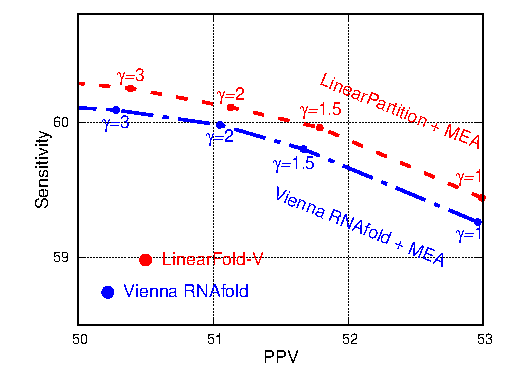
\includegraphics[scale=.7]{figs/new_MEA_diff_gamma_beam_inf_threshold_001}
&
\raisebox{-0.25cm}{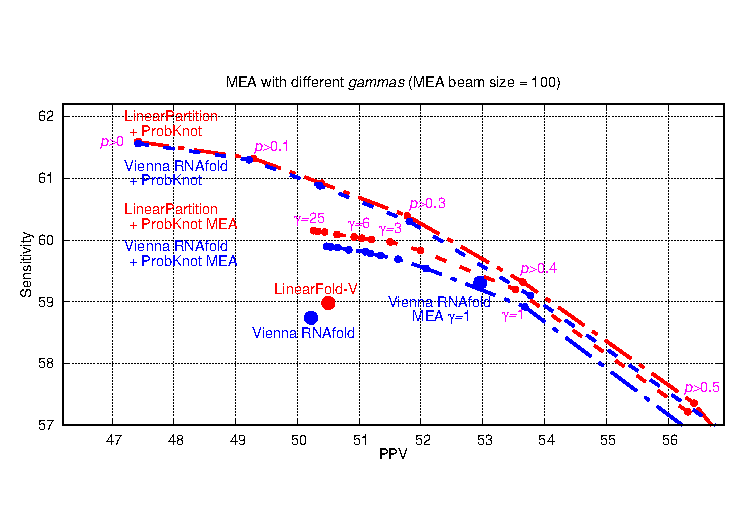
\includegraphics[scale=.58]{figs/MEA_gamma_B100}}

\end{tabular} % A: specify MFE in label
\caption{Accuracy comparison for two systems.
	{\bf A}: Overall MFE and MEA structure PPV-sensitivity tradeoff of two systems with varying $gamma$. 
	{\bf B}: Overall ThreshKnot structure PPV-sensitivity tradeoff of two systems with varying $gamma$
	% {\bf C}:
	\linearpartition even leads to a small improvement in the downstream MEA predictoin using the probability matrix computed in linear time.
	\label{mea}
}
\end{figure*}

\iffalse
\begin{figure*}[t]
\center
\begin{tabular}{ccc}
\hspace{-0.5cm}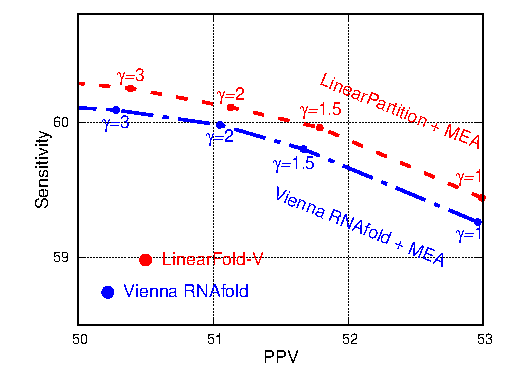
\includegraphics[scale=.8]{figs/new_MEA_diff_gamma_beam_inf_threshold_001}
&
\hspace{-1.85cm}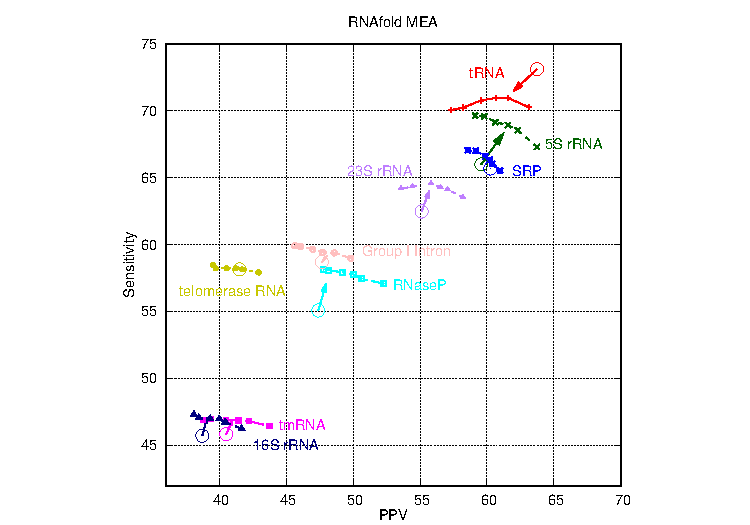
\includegraphics[scale=.58]{figs/new_MEA_RNAfold_diff_gamma_families}
&
\hspace{-2.35cm}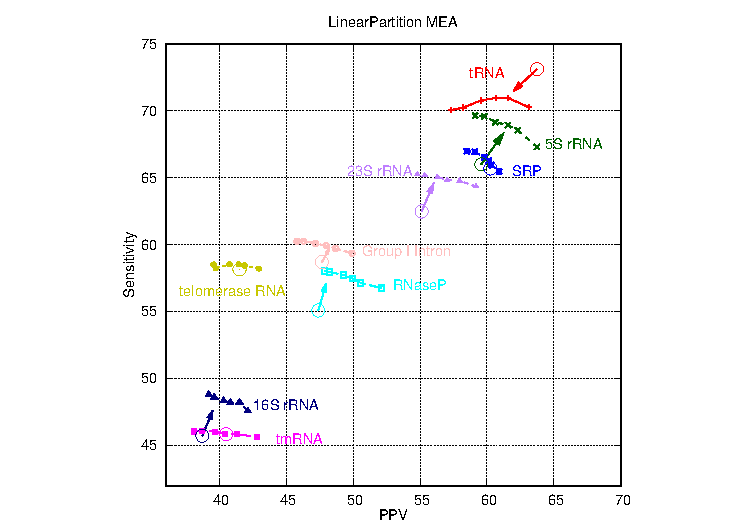
\includegraphics[scale=.58]{figs/new_MEA_LinearPartition_diff_gamma_families}

\end{tabular} % A: specify MFE in label
\caption{MFE and MEA structure accuracy comparison for two systems.
	{\bf A}: Overall PPV-sensitivity tradeoff of two systems with varying $gamma$. 
	{\bf B}:
	{\bf C}:
	\linearpartition even leads to a small improvement in the downstream MEA predictoin using the probability matrix computed in linear time.
	\label{mea}
}
\end{figure*}
\fi

We next compare accuracy of \linearpartition with the baseline \viennarnafold.
We take the base pair probability matrices from these two systems, 
and fed them to standard MEA algorithm.
We use Positive Predictive Value (PPV, the fraction of predicted pairs in the known structure) and sensitivity (the fraction of known pairs predicted) to measure the accuracy across all families, as well as slipping method to allow base pair to slip by one nucleotide \cite{sloma+mathews:2016}.


% Figure~\ref{mea} shows that \linearpartition even leads to a small improvement in the downstream MEA predictoin using the probability matrix computed in linear time. 
% Figure~\ref{mea} gives the accuracy comparison between 
Figure~\ref{mea}A shows that 
(1) MEA-based method is more accurate than MFE-based method for both systems; 
(2) \linearpartition + MEA is constantly more accurate than \viennarnafold + MEA.
With the same $\gamma$, a hyperparameter balances PPV and sensitivity in MEA algorithm,
\linearpartition + MEA enjoys a small improvement in both PPV and sensitivity.


% ThreshKnot
Probknot is another partition-function-based method which is much simpler than MEA, only adds a linear post-processing step after the partition function calculation, and can predict pseudoknots. 
Recently, ThreshKnot \cite{Liang+:2019}, a simple thresholded version of ProbKnot, 
leads to more accurate overall predictions by filtering out unlikely pairs whose prob falls under a given threshold,
so we also compare ThreshKnot structure accuracy.

Figure~\ref{mea}B shows that ???????

per family accuracy

% Figure 3B shows that LinearFold is more accurate than the baselines, and interestingly, this advantage is more pronunced on longer sequences, esp. the two longest families in the database, 16S and 23S Ribosomal RNAs.

\iffalse
\begin{figure}[H]
\center
\begin{tabular}{cc}
\multicolumn{2}{c}{\hspace{-1cm}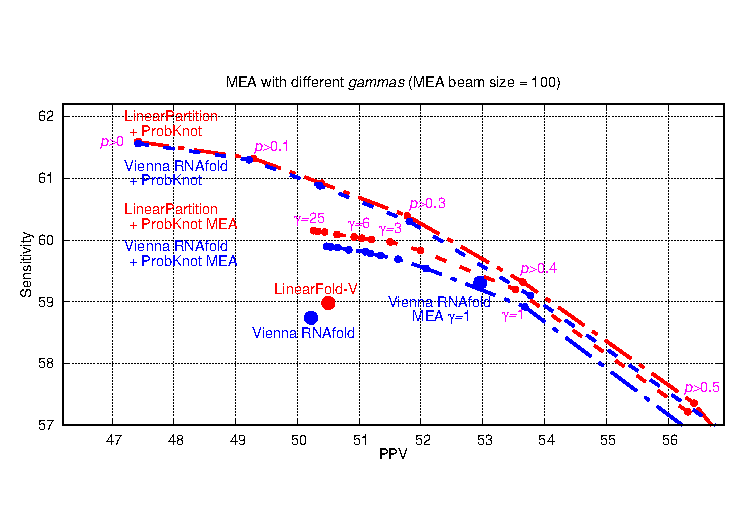
\includegraphics[scale=.7]{figs/MEA_gamma_B100}}
\\
\hspace{-0.5cm}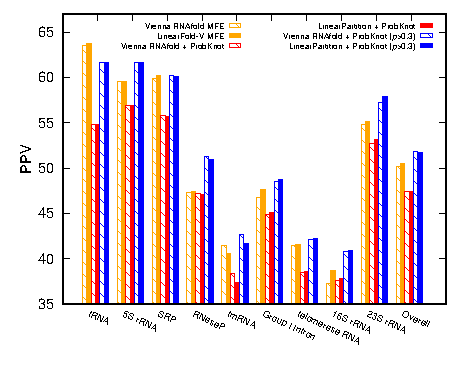
\includegraphics[scale=.68]{figs/ProbKnot_PPV}
&\hspace{-0.5cm}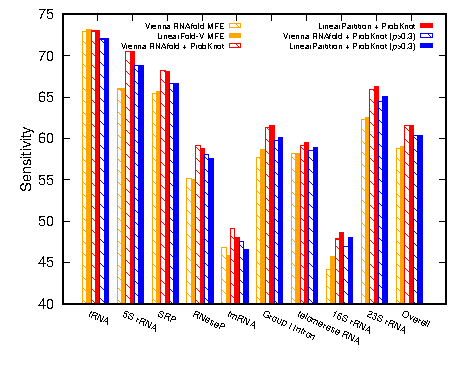
\includegraphics[scale=.68]{figs/ProbKnot_Sens}
\end{tabular}
\caption{ThreshKnot structure accuracy comparison.
	{\bf A}
	{\bf B}
	{\bf C}
	\label{probknot}
}
\end{figure}
\fi



\subsection{Search Quality}

Fig. 4A–B show that our \linearpartition algorithm can indeed approximate the partition function reasonably well. 
Here we measure root-mean-square deviation (RMSD) between the two probability matrices $p$ and $p'$ (from Vienna RNAfold and \linearpartition, resp.) 
over the set of all possible pairs pairs($x$) on a sequence $x$ (i.e., ${\rm{pairs}}(x)={1\leq{i}<j\leq{|x|} \ | \  x_{i}x_{j} \in {\rm CG, GC, AU, UA, GU, 
UG},j-i>3}$): 

\begin{equation}
{\rm{RMSD}}(p,p')=\sqrt{\frac{1}{|{\rm{pairs}}(x)|}\sum_{(i,j) \in {{\rm{pairs}}(x)}}{(p_{i,j}-p'_{i,j})}^2}
\end{equation}

\begin{figure*}[t]
\center
\begin{tabular}{cc}
\panel{A} & \panel{B} \\[-0.4cm]
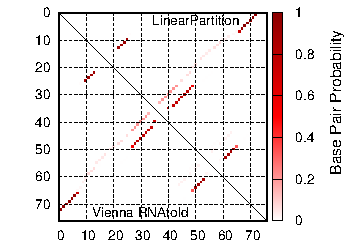
\includegraphics[width=0.3\textwidth]{figs/tRNA_identical_heatmap}
&
{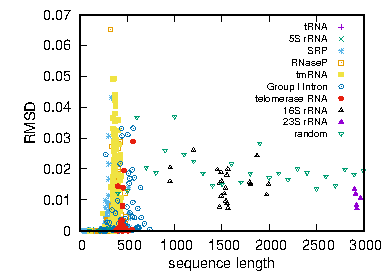
\includegraphics[width=0.38\textwidth]{figs/rmsd_family_plus_random_b2}}
\\[-0.2cm]
\panel{C} & \panel{D}\\[-0.5cm]
\hspace{-0.5cm}\raisebox{-0.45cm}{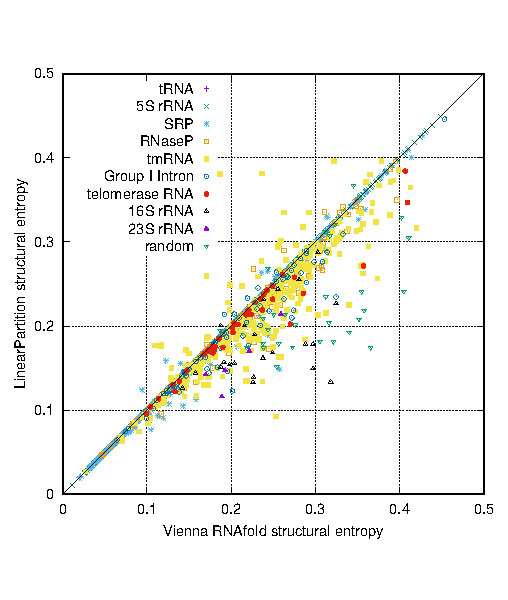
\includegraphics[width=0.28\textwidth]{figs/structure_entropy_xy_plus_random}}
&
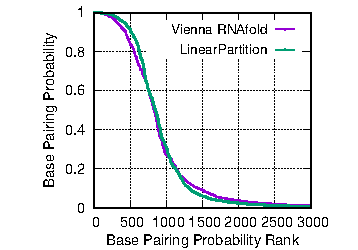
\includegraphics[width=0.38\textwidth]{figs/sorted_prob_23s}
\end{tabular}
\caption{
Comparison of base pair probabilities from \viennarnafold and \linearpartition.
	{\bf A}: \linearpartition (upper triangle) and Vienna RNAfold (lower triangle) result in identical base pair probability matrix for {\it E.~coli} tRNA$^\textit{Gly}$.
	{\bf B}: root-mean-square deviation (RMSD) is relatively small between \linearpartition and Vienna RNAfold.
	{\bf C}: structural entropy comparison.
	{\bf D}: \linearpartition starts higher and finishes lower than RNAfold in a sorted probability curve for \ecoli 23S rRNA.
	\label{sq}
}
\end{figure*}

Figure~\ref{sq}A shows the probability matrix for short sequence, e.g. tRNA sequence, from both RNAfold and \linearpartition yield identical matrices (i.e., RMSD=0). Figure~\ref{sq}B shows that RMSD is relatively small across all RNA families in the ArchiveII dataset. The highest deviation is 0.067 for one RNaseP sequence, which means on average, each pair’s probability deviation in that worst-case sequence is about 0.067 between the exact algorithm and our linear-time one. With sequence length increasing, RMSD gradually decreases, since the number of possible pairs grows in $O(n^2)$ but the number of highly probable pairs grows in $O(n)$; on the longest 23S rRNA family, RMSD is about 0.015. We also included 30 random RNA sequences with length 100–3,000 and they behave similarly to natural sequences in terms of RMSD. 

% Figure~\ref{sq}C and D show
We assume \linearpartition base pair probability distribution is peakier since it ignores low energy substructure in partition function calculation.
We uses structural entropy \cite{Huynen+:1997} to measure this, 
where lower structural entropy indicates that the distribution is dominated by fewer base pairing probabilities.
Figure~\ref{sq}C shows \linearpartition distribution is peakier (lower structural entropy) than RNAfold for most sequences.

We also uses \ecoli 23S rRNA as an example to illustrate the distribution difference.
We sort all base pair probabilities from high to low and take the top 3,000 rank.
Figure~\ref{sq}D shows \linearpartition probability distribution curve starts higher and finishes lower.


\subsection{Beam Size Impact}



\begin{figure}[H]
\center
\includegraphics[width=0.48\textwidth]{figs/RMSD_beamsize}
\end{figure}

\subsection{Example}




\label{sec:discussion}
% !TEX root = \linearpartition.tex

\subsection{Summary}



\subsection{Analysis}


\subsection{Extensions}

Our algorithm has several potential extensions.

\begin{enumerate}
\item 
We will linearize the partition function-based heuristic pseudoknot prediction methods such as ProbKnot, IpKnot, and Dotknot by replacing their bottleneck $O(n^3)$-time calculation of the partition function with our LinearPartition. 
All these heuristic methods uses rather simple heuristic criteria to choose pairs from the base pair probability matrix. 
For example, the second step of probknot selects base pairs $(i,j)$ where the $i–j$ pairing probability is the largest for both bases $i$ and $j$. 
This might appear as $O(n^2)$ in the worst case, 
but since the linear-time beam search used in \linearpartition only returns $O(nb)$ pairs where $b$ is the constant beam size, 
this second step is still $O(n)$, 
giving an overall linear-time method, LinearProbKnot. 
We can similary get LinearIPknot, LinearProbknot and LinearDotKnot, etc.
With these promising substantial results of \linearpartition, 
we believe LinearProbknot (and LinearIPknot, LinearDotKnot, etc) should be as accurate as, if not more accurate than, their original $O(n^3)$ versions.

\item Accelerate and Improve bimolecular and multistrand structure prediction.
\linearpartition provide important new ways to improve existing bimolecular and multistrand structure prediction algorithm such as AccessFold \cite{DiChiacchio+:2016}. 
\linearpartition will provide a much faster solution to the accessibility calculation.
Also, \linearpartition will help include predictions of intramolecular and bimolecular pairs, re
 have immediate impact on our ability to predict bimolecular structures by improving speed and also providing additional structure information to users.


\end{enumerate}





Aim 3b: Accelerate and Improve bimolecular and multistrand structure prediction
Many ncRNAs function by interacting with other RNA sequences by base pairing. We developed several software tools for predicting base pairing structures between two sequences (bimolecular) [81, 68, 23, 24]. There are two important barriers to accurate bimolecular structure prediction. First, RNA sequences form self-structure that prevents bimolecular structure prediction. We account for this in our AccessFold algorithm, which is part of the RNAstructure software package and uses a partition function calculation to approximate the accessibility [23] The second barrier is that many simple bimolecular structures that also include unimolecular pairs, such as the kissing hairpin [13], are tantamount to pseudoknots in our algorithms.

The linear algorithms from aims 1 and 2 provide important new ways to improve our existing AccessFold algo- rithm. First, the linear partition function calculation (Aim 1a) will provide a much faster solution to the accessibility calculation. Second, the linear pseudoknot prediction (aim 2) will provide us with the algorithm needed to elevate AccessFold to include predictions of intramolecular and bimolecular pairs. Currently, AccessFold only provides the pairs between strands, ignoring the pairs within a strand.
We will advance AccessFold to incorporate the new algorithms from aims 1 and 2 and test it against a database of bimolecular structures we developed previously [23]. This will have immediate impact on our ability to predict bimolecular structures by improving speed and also providing additional structure information to our users.

%\vspace{-.2cm}
% \label{sec:methods}
% % !TEX root = main.tex

% \setcounter{figure}{0}
% \renewcommand{\thefigure}{Online Method \arabic{figure}}
% \setcounter{table}{0}
% \renewcommand{\thetable}{Online Method \arabic{table}}

\section*{Methods}

\small

\subsection*{Datasets}

We use sequences from two datasets, ArchiveII and RNAcentral.
The archiveII dataset 
(available in \url{http://rna.urmc.rochester.edu/pub/archiveII.tar.gz}) is % \cite{sloma+mathews:2016}, 
a diverse set with 3,857 RNA sequences and their secondary structures.
It is first curated in the 1990s to contain sequences with structures that were well-determined by comparative sequence analysis~\cite{mathews+:1999}% [72] 
and updated later with additional structures~\cite{sloma+mathews:2016}. % [96].  
% and is available in \url{http://rna.urmc.rochester.edu/pub/archiveII.tar.gz}.
We remove 957 sequences that appear both in the ArchiveII and the S-Processed datasets~\cite{Andronescu+:2007}, because CONTRAfold uses S-Processed for training. 
We also remove all 11 Group II Intron sequences 
because there are so few instances of these that are available electronically.
Additionally, we removed 30 sequences in the tmRNA family because the annotated structure for each of these sequences contains fewer than 4 pseudoknots, 
which suggests the structures are incomplete. 
These preprocessing steps lead to a subset of ArchiveII with 2,859 reliable secondary structure 
% RNA sequence and structure pairs 
examples 
distributed in 9 families. 
See~\ref{tab:archiveII} for the statistics of the sequences we use in the ArchiveII dataset.
% But since CONTRAfold (v2.02) machine-learned model is trained on the S-Processed dataset \cite{},
% we removed those overlap sequences. 
% As in \linearfold paper, we also remove those sequences CONTRAfold (v2.02) used for training.
% The remaining dataset contains 2889 RNA sequences from 9 families, 
% with average length 222 $nt$ and max length 2968 $nt$.
Moreover, we randomly sampled 22 longer RNA sequences (without known structures) from RNAcentral 
% (The RNAcentral Consortium, 2017) 
(\url{https://rnacentral.org/}),
with sequence lengths ranging from 3,048~{\it nt} to 244,296~{\it nt}.
For the sampling, we evenly split the range from $3,000$ to $244,296$ (the longest) into 24 bins by log-scale, and for each bin we
randomly select a sequence (there are bins with
no sequences).
% (Homo Sapiens Transcript NONHSAT168677.1, from the NONCODE database (Zhao et al., 2016)).
% We run all experiments 
% % (compiled by GCC 4.9.0) 
% on a Linux machine, 
% with 2.90GHz Intel Core i9-7920X CPU and 64G memory.

To show the approximation quality on random RNA sequences, 
we generated 30 sequences with uniform distribution over \{A, C, G, U\}.
% The lengths of these sequences are 100, 200, ..., 3000.
The lengths of these sequences are spaced in 100 nucleotide intervals from 100 to 3,000.
% with lengths range from 100~{\it nt} to 3,000~{\it nt}. 


\subsection*{Baseline Software}
% We present two versions of \linearpartition, \linearpartitionv and \linearpartitionc.
% \linearpartitionv uses the experiment-based thermodynamic parameters~\cite{mathews+:1999,Mathews+:2004,xia+:1998}
% as implemented in 
We use two baseline software packages: 
(1) \viennarnafold %~\cite{lorenz+:2011}
(Version 2.4.11) 
from 
\url{https://www.tbi.univie.ac.at/RNA/download/sourcecode/2_ 4_x/ViennaRNA-2.4.11.tar.gz} 
and 
(2) \contrafold %~\cite{do+:2006}
(Version 2.0.2) 
from
\url{http://contra.stanford.edu/}.
\viennarnafold is a widely-used RNA structure prediction package,
while \contrafold is a successful machine learning-based RNA structure prediction system.
Both provide partition function and base pairing probability calculations based on 
the classical cubic runtime algorithm.
Our comparisons mainly focus on the systems with the same model, 
i.e., \linearpartitionv vs. \viennarnafold and \linearpartitionc vs. \contrafold.
In this way the differences are based on algorithms themselves rather than models.
% bugs in contrafold
We found a bug in \contrafold by comparing our results to CONTRAfold, 
which led to overcounting multiloops in the partition function calculation.
We corrected the bug, and all experiments are based on this bug-fixed version of \contrafold.


\subsection*{Evaluation Metrics and Significance Test}

Due to the uncertainty of base-pair matches existing in comparative analysis
and the fact that there is fluctuation in base pairing at equilibrium,
we consider a base pair to be correctly predicted if it is also displaced by one
nucleotide on a strand~\cite{mathews+:1999}.
Generally, if a pair $(i,j)$ is in the predicted structure, we consider it a
correct prediction if one of $(i,j)$, $(i-1,j)$, $(i+1,j)$, $(i,j-1)$, $(i,j+1)$ is in the
ground truth structure.
% We also report the accuracy using exact base pair matching instead of this
% method, in Figure~\ref{tab:accuracy_nos}. 
%To evaluate the accuracy, 
% Both sensitivity and PPV are reported.
%Positive Predictive Value
%(PPV), 

We use Positive Predictive Value (PPV)
and sensitivity 
as accuracy measurements. 
Formally, denote $\vecy$ as the predicted structure and $\vecy^{*}$ as the ground
truth, we have:
% $\ppv = \frac{\text{true positives}}{\text{true positives} +
%   \text{false positives}} = \frac{|\vecy \cap \vecy^*|}{|\vecy|} $
% $ \sens = \frac{\text{true positives}}{\text{true positives} +
%   \text{false negatives}} =
% \frac{|\vecy \cap \vecy^*|}{|\vecy^*|}$

$$\ppv = \frac{\#_{\text {TP}}}{\#_{\text {TP}} + \#_{\text {FP}}}  = 
\frac{|\pairs(\vecy) \cap \pairs(\vecy^*)|}{|\pairs(\vecy)|} $$

$$ \sens = \frac{\#_{\text {TP}}}{\#_{\text {TP}} + \#_{\text {FN}}}  =
\frac{|\pairs(\vecy) \cap \pairs(\vecy^*)|}{|\pairs(\vecy^*)|}$$
where $\#_{\text {TP}}$ is the number of true positives (correctly predicted pairs),
$\#_{\text {FP}}$ is the number of false positives (wrong predicted pairs)
and $\#_{\text {FN}}$ is the number of false negatives (missing ground truth pairs).

We test statistical significance using a paired, two-sided permutation test~\cite{Aghaeepour+Hoos:2013}.
We follow the common practice, choosing $10,000$ as the repetition number
and $\alpha=0.05$ as the significance threshold.
% following previous work~\cite{Aghaeepour+Hoos:2013}.

\subsection*{Curve Fitting}
We determine the best exponent $a$ for the scaling curve $O(n^a)$ for each data series in Figures~\ref{fig:linearpairs} and \ref{fig:runtime}.
Specifically, we use $f(x) = a x + b$ to fit the log-log plot of those series in Gnuplot;
e.g., fitting $\log t_n = a \log n + b$, where $t_n$ is the running time on a sequence of length $n$,
so that $t_n = e^b n^a$.
Gnuplot uses the nonlinear least-squares Marquardt-Levenberg algorithm.


\section*{Code availability}\label{code}

Our \linearpartition source code can be downloaded  from\\ 
{\tt\url{https://github.com/LinearFold/LinearPartition}}.

\section*{Data availability}

%\small

The data that support the findings of this study are available from the corresponding author upon request.

%% The data sets used in this study are  available online:
%% ArchiveII~data~set: {\small\url{http://rna.urmc.rochester.edu/pub/archiveII.tar.gz}};
%% RNAcentral data~set: \url{https://rnacentral.org}.
%by requesting from the corresponding
%author.


% \section*{Code availability}\label{code}

% Our \linearpartition source code can be downloaded  from\\ 
% {\tt\url{https://github.com/LinearFold/LinearPartition}}.

% \section*{Data availability}

%\small

% The data that support the findings of this study are available from the corresponding author upon request.

%% \label{sec:data}
%% % !TEX root = main.tex

\section*{Data availability}

\small

The data sets used in this study are available online:
ArchiveII data set: \url{};
RNAcentral data set: \url{}.
%by requesting from the corresponding
%author.


% \showmatmethods{
%   % \ssmall
%   \section*{Methods}
%   \label{sec:method}  
% Detailed description of our algorithms, datasets, and evaluation metrics %statements of data availability and any associated accession codes and references,
% are available in the online version of the paper. 
% % % !TEX root = linearpartition.tex

\setcounter{figure}{0}
\renewcommand{\thefigure}{Online Method \arabic{figure}}
\setcounter{table}{0}
\renewcommand{\thetable}{Online Method \arabic{table}}

\section*{Online Methods}

%We propose LinearFold,
%% LinearFold is 
%% a linear-time prediction algorithm predicting RNA
%% secondary structures.
% Our \linearfold approach is 
% presented in four steps, starting from
% the most naive but easy-to-understand exhaustive search version (Fig.~\ref{fig:method} C1), and gradually 
% build it up to 
% the linear-time version (Fig.~\ref{fig:method} C4), using a stack-top merge and beam search.

Here we first formulate the \linearfold algorithm more formally.

\subsection*{Formulation}
%% The RNA secondary structure prediction problem can be formalized as follows,
%% using the dot-bracket format to represent structures.
Generally, given an input RNA sequence
$$ \vecx = x_1x_2\ldots x_{n}, \text{ where } x_i \in \{\tt{A},\tt{C},\tt{G},\tt{U}\},$$
the RNA secondary structure prediction algorithm
%$\mathit{f}$ 
aims to find the best-scoring pseudoknot-free structure
%$$ \vecy = y_1y_2\ldots y_{n}, \text{ where } y_i \in \{\md, \ml, \mr\}$$
%(to address pseudoknots, different types of brackets would be required)
according to a scoring function \score (e.g., model score or negative free energy) parameterized by model $\weight$:
% (or minimum model cost):
\vspace{-0.1cm}
% \begin{equation}
%   %f(\vecx) =
%   \argmax_{\vecy \in \GEN(\vecx)} \score(\vecx, \vecy; \weight)
%   \label{eq:mfe}
% \end{equation}
%\vspace{-0.2cm}
where $\GEN(\vecx)$ is the set of all possible pseudoknot-free structures
\[
\GEN(\vecx) =
\big\{\vecy \in \{\md, \ml, \mr\}^n \;\mid\; \vecy \text{~is balanced in brackets}\big\}.
\]
%and %$\score$ is the cost function (i.e., free
%energy function), and
The two baselines in our study, \contrafold
and \viennarnafold, use scoring functions that are very similar  in structure, % scoring functions,
but very different in parameters 
(the former learns \vecw from data, % in which the free energy
%is not revealed,
while the latter is based on thermodynamics).

All dynamic programming-based prediction algorithms, including ours, %like previous ones, are based on dynamic programming,
require the scoring function to {\em decompose} to the scorings of smaller structures,
in order to have efficient computation.
For example, the main text (see Fig.~\ref{fig:method}) uses the simplest Nussinov-style scoring function 
that factors to each individual base pair and simply counts the number of pairs in a structure:
\begin{equation}
  \score_{\text{Nussinov}}(\vecx, \vecy; \_) = \# \pairs(\vecy) = \sum_{(i,j)\in \pairs (\vecy)} 1
  \label{eq:nussinov}
\end{equation}
where $\pairs(\vecy)$ returns the list of base pairs in \vecy, e.g.,
$\pairs(\text{``\md\ml\ml\md\mr\mr\md''}) = \{(2,6), (3,5)\}$.
Note this scoring function does not depend on any model,
but we could in principle assign different scores in \vecw for GC, AU, and GU pairs (e.g., $w_\text{GC} > w_\text{AU} > w_\text{GU}$),
and also introduce a penalty for each unpaired nucleotide ($w_\unpaired < 0$),
which we call the ``Extended Nussinov'' model:
\begin{equation}
  \score_{\text{extended}}(\vecx, \vecy; \vecw) = \sum_{(i,j)\in \pairs (\vecy)} w_{x_i x_j} +\sum_{i\in \unpaired(\vecy)} w_\unpaired
  \label{eq:extended}
\end{equation}
In reality, the actual scoring functions % $\score$ (scoring structure \vecy on input \vecx by model \vecw) can be
used by \contrafold, \rnafold, and \linearfold are more complex and they
decompose to individual loops: % as follows:
\begin{equation}
  \begin{split}
 \score_\text{real}(\vecx, \vecy; \weight) = &
 \!\!\!\!\sum_{h \in \text{hairpin\_loops}(\vecy)}\!\!\!\! \score^{\mathrm H}(\vecx, h; \weight)  + \!\!\!\!\sum_{s \in \text{single\_loops}(\vecy)}\!\!\!\! \score^{\mathrm S}(\vecx, s; \weight) \\
 + & \!\!\!\!\sum_{m \in \text{multi\_loops}(\vecy)}\!\!\!\! \score^{\mathrm M}(\vecx, m; \weight) +  \!\!\!\!\sum_{e \in \text{external\_loops}(\vecy)}\!\!\!\!\!\!\!\! \score^{\mathrm E}(\vecx, e; \weight).
\end{split}
\label{eq:decomp}
\end{equation}
The thermodynamic %minimal free energy
model in \viennarna scores %, the score of constructing 
each type of loop %(hairpin, single-branch, multi-branch, and external)
using several feature templates such as
hairpin/bulge/internal loop lengths,
terminal mismatches, helix stacking, helix closing, etc.
%% %the following feature components:\cite{mathews+:1999}
%% \begin{itemize}[itemsep=-1mm]
%% \item %$\score^{\mathrm H}(\cdot,\cdot;\cdot)$,
%% Hairpin loops: hairpin length, terminal mismatch, and special tri-, tetra-, and hexa-loops. 
%% \item %$\score^{\mathrm S}(\cdot,\cdot;\cdot)$,
%% Single-branch loops (including helix stacking as empty loop, and bulge and internal loops):
%% bulge length, internal loop length, internal loop left-right balancing,
%% terminal mismatch, helix stacking, and helix closing.
%% \item %$\score^{\mathrm M}(\cdot,\cdot;\cdot)$,
%% Multi-branch loops: multi-loop base cost, terminal mismatch,
%% left/right dangles, multi paired, and multi unpaired.
%% \item %$\score^{\mathrm E}(\cdot,\cdot;\cdot)$,
%% External loops: left/right dangles, external paired and external  unpaired. 
%% \end{itemize}
The machine-learned model in \contrafold
replaces energies in the above framework with model weights learned from data.
%all the model weights are learned from data, instead of the free energy.
%% We conclude
%% the cost decomposition in Fig.~\ref{fig:realdeduct}. 

%% RNA secondary structure prediction is regarded as a challenging problem,
%% that no existing model can score perfectly to match the actual
%% structure with the minimum free energy (or minimum model cost) function, i.e.,
%% {\bf imperfect modeling}.
%% Consider $y^*(\vecx)$ as the actual secondary structure of the given sequence,
%% and an evaluation metric (e.g., PPV, sensitivity) $M$ to
%% calculate accuracy of a set of predicted structures against the actual
%% structures ($M(y,y)=1$), we are likely to have $M(f(\vecx), y^*(\vecx)) < 1$
%% according to the existing results reported(see Fig.\ref{fig:accuracy}).

%% Our proposed \linearfold algorithm can linearize any system with a variant of
%% $(\score,\weight)$, as long as $f(\vecx) = \argmin_{\vecy \in \GEN(\vecx)}
%% \score(\vecx, \vecy; \weight)$ can be 
%% solved in cubic-time by the dynamic programming algorithm.
%% The linearization maintains the same cost function and model $(\score,\weight)$,
%% but the objective function is different, i.e. $f' \neq f$, as we set a series of
%% soft constraints
%% during the beam search, pruning out structures with high cost or high free
%% energy which depends on the given $(\score,\weight)$.
%% Experimental results show that
%% this difference leads to a higher accuracy in linearizing \contrafold and
%% Vienna RNAfold (see Fig.~\ref{fig:accuracy} and Fig.~\ref{fig:beamsize}).

Our \linearfold algorithm can ``linearize'' any cubic-time prediction system
as long as the scoring function decomposes in a way similar to Eqs.~\ref{eq:nussinov}--\ref{eq:decomp} above.
Below we formalize our \linearfold algorithm step by step, % as follows.
using the Extended Nussinov model in Eq.~\ref{eq:extended} to strike a balance between simplicity
and reality.
We will refer to both the high-level illustration in Fig.~\ref{fig:method},
and a more formal deductive system in Fig.~\ref{fig:deduction}.

% The basic idea of our proposed

% We propose \linearfold, the first global linear-time RNA secondary structure
% prediction algorithm. 
% The basic idea of linear-time prediction is to predict incrementally from
% left to right,
% %, inspired by human sentence processing. To adapt it to RNA
% %sequences, 
% %we view the problem as incrementally converting the RNA sequence into
% %the dot-bracket format, such that 
% labeling each nucleotide  as unpaired ``{\textbf .}'', opening ``{\textbf (}'',
% or closing ``{\textbf )}''. 
% %% This makes the
% %% dot-bracket format equivalent to the pseudoknot-free RNA secondary structures
% We require this dot-bracket string to be well-balanced as we only consider pseudoknot-free structures
% (to address pseudoknots, different types of brackets would be required. This is left as our future work). 

% the term "exponentially traverse" is strange, I suggest "traverse all possible
% structures in GEN(\vecx), which takes exponenential time
%% 4-step method claim
%\vspace{.25cm}
\subsection*{Naive exhaustive incremental prediction: $O(3^n)$ time}
By exhaustively predicting $y$ from left-to-right, we
traverse all the possible structures in $\GEN(\vecx)$,
% calculate the free energy for each of them,
and pick the one with the highest score (or lowest free energy). % or model cost.
We denote each {\em state} at step $j$ ($j \in \{0,\ldots, n\}$)
as a tuple along with a score $s$:
%\begin{equation}
\[
        \nnitem{\vecy}{\sigma}{j}{s},
\]
%$s = \nitem{{\bm \sigma} | i}{j}\vecy$,
%\end{equation}
where \vecy is the (sub)structure for the prefix $x_1 \ldots x_j$,
and
$\sigma$ is the  stack consisting of unmatched opening bracket positions in \vecy.
For the Nussinov model, score $s$ is simply the number of pairs in \vecy.
For example, if \vecy=``\md\ml\ml\md\mr\ml'', then $\sigma=[2,6]$ and $s=1$.
%and $s$ is the score of the state.
%% so far
%% where $i$ is the top of the stack, meaning $x_i$ is the last unmatched opening nucleotide. 
%$\vecy$ is the corresponding dot-bracket (sub)sequence up to $x_{j-1}$.
Each state can transition into a subsequent state, taking one of the three
actions:
\begin{enumerate}
\itemsep-0.2em
\item \push:
$\nnitem{\vecy}{\sigma}{j}{s} \goesto \nnitem{\vecy\!\circ\!{\text `}\ml{\text '}}{\sigma | j}{j+1}{s}$.
%which labels the current nucleotide $x_j$ as a left bracket ``{\textbf (}'', 
%putting it on top of the stack;
\item \nskip:
$\nnitem{\vecy}{\sigma}{j}{s} \goesto \nnitem{\vecy\!\circ\!{\text `}\md{\text '}}{\sigma}{j+1}{s + w_\unpaired}$.
%, which labels $x_j$ as a dot ``{\textbf .}'', leaving the stack unchanged,
%and 
\item \pop:
$\nnitem{\vecy}{\sigma | i}{j}{s} \goesto \nnitem{\vecy\!\circ\!{\text `}\mr{\text '}}{\sigma}{j+1}{s+ w_{x_i, x_j}}$
(if $x_i$ and $x_j$ can form a base pair).
%, which labels $x_j$ as a right bracket ``{\textbf )}'', 
%if it matches $x_i$
%nucleotide with $x_{\TOP}$, the top of the stack, 
%and popping $i$ from the stack.
\end{enumerate}
See Fig.~\ref{fig:deduction}(a) for the deductive system.
% labeled dot-bracket sequences ($|y|=j$).
% Then the prediction algorithm
% starts with \(\nitem{\sigma_{\epsilon}}{0}{\epsilon}\), and ends with
% $|\GEN(x)|$ different states,
% \begin{equation}
%   \nitem{\sigma_{\epsilon}}{n}{y} ,y \in \GEN(x).
% \end{equation}
%% Starting at the state \(\nitem{\sigma_{\epsilon}}{0}{\epsilon}\), it takes
This algorithm takes $O(3^n)$ time to exhaustively traverse all possible
%structures (see the first part of Figure~\ref{fig:method}).
structures (see Figure~\ref{fig:method}D1).

% we start with an empty structure, with the current
% index at the beginning of the sequence, 
% The algorithm is
% with $O(3^n)$ time. 

% the structure $y \in \GEN(x)$ satisfies $y =y_1y_2...y_n, y_i \in \{\textbf{. (
%   )}\}$, with a balanced of brackets. We note $\pair(y) = \{(i,j) | (y_i,y_j)
% \text{~matches~in~brackets}\}$. 

% Now, given an free energy function
% $\energy$ and a model $\weight$ , our algorithm is to find the structure with
% the minimum free energy,

% we view the problem as incrementally converting the RNA sequence into the
% dot-bracket format, that each nucleotide can be labeled as unpaired ``{\tt .}'' (a
% skip action), opening ``{\tt (}'' (a push action), or closing ``{\tt )}'' (a pop
% action). The naive exhaustive prediction method would seem to require $O(3^n)$
% time, as there are 3 different labels for each nucleotide.

%\vspace{.25cm}
\subsection*{Dynamic Programming via Identical-Stack Merging:
  $O(2^{n})$ time}

Now we apply dynamic programming on top of this exhaustive method to exploit
shared computations.
Consider a simple case that two states can be merged: if
there are two states in the same step $j$,
% $\nitem{\bm \sigma}{j}\vecy$ and $\nitem{\bm \sigma}{j}{\vecy'}$, 
% sharing the exact same stack $\bm \sigma$ but with different dot-bracket strings $\vecy$ and $\vecy'$, 
%i.e.,
%they have the same positions of all unpaired openings %, means that they have identical stacks, 
we say that these two states are ``equivalent'' and we can merge them
(and only keep the better scoring between \vecy and $\vecy'$). 
%A merged state can be represented as $\twotuple{\bm \sigma}{j}$. 
Fig.~\ref{fig:method}B(Idea 1)/D2 illustrates this merging and
Fig.~\ref{fig:deduction}(b) shows the deductive system. 
Although we merge to reduce the number of states, it is still exponential time, 
% use fewer states to process, the number of
% possible states are still exponential,
since there could be exponentially many
different stacks in each step. 
% against the current index $j$.
This algorithm takes $O(2^{n})$ time. 
%%  for every possible stack
%% $\twotuple{\bm \sigma}{j}$ considered in the prediction process.

%\vspace{.25cm}
\subsection*{Dynamic Programming via Stack Top Packing: $O(n^3)$ time}

To avoid considering exponentially many states, 
we further
%% further apply the
%% Graph-Structured Stack (GSS, \cite{Tomita:1988}) to the dynamic programming. 
pack states with different stacks.
Consider two states in the same step $j$,
% $\twotuple{{\bm \sigma_0} | i}{j}$ and $\twotuple{{\bm \sigma_1} | i}{j}$,
which share the last unpaired opening $i$ (i.e., stack top). 
%(where $i$ is the same top of the stack).
We call these states ``temporarily equivalent'', since they can be treated as
exactly the same until the unpaired opening $x_i$ is closed (and thus popped from the stack).
% In other words we can represent both stacks ${\bm \sigma_0} | i $ and ${\bm \sigma_1} | i$
as $...i$, where $...$ denotes part of the history that we do not need at this moment.
This factorization of stacks is called ``Graph-Structured Stacks'' (GSS) by Tomita. \cite{Tomita:1988}
After packing, we define the new state to be $\tuple{i,j}$
%In our dynamic programming prediction algorithm, 
and therefore we  maintain $O(n^2)$ states.
For each state $\tuple{i,j}$, the pop action
can take worst-case $O(n)$ time because $\tuple{i,j}$ can combine with every $\tuple{k,i}$ from step $i$.
%due to the graph-structured stack. 
Thus the overall time complexity is $O(n^3)$.
See Fig.~\ref{fig:method}B(Idea 2)/D3 for  
an example of the packing process
and Fig.~\ref{fig:deduction}(c,d)
for the deductive system.

Now we explain the
packing on these ``temporarily equivalent'' states in detail. 
We use the GSS \cite{Tomita:1988} to pack and unpack
them, which has been widely used in parsing natural language sentences.
\cite{huang+sagae:2010}
% The idea is to combine
The idea behind the packing process is to combine the left structure information
of different states packed together in the push action,
and this structure is later unpacked in the future pop action.

Basically, if state $r$ generates state $s$ by a push action, then $r$ is added
onto $\pi(s)$, a set of predictor states. When two equivalent pushed states get
packed, we combine their predictor states. For example, if $r_x =
\tuple{t_x, j}$ predicts $s = \tuple{j,j+1}$ for $x\in \{0,\ldots, k\}$, then $\pi(s) =
\{r_x|x=0 \ldots k\}$. 
% In the pop step, state $s = \tuple{i,j}$ tries to combine with every predictor
% state $r \in \pi(s)$, and the resulting state $t$ inherits the predictor states
% set from $r$, i.e., $\pi(t) = \pi(r)$. 
To pop state $s = \tuple{i,j}$, we combine it with each of its predictor states
$r \in \pi(s)$ to make a resulting state $t$.
$t$ inherits the predictor states from $r$, i.e., $\pi(t) = \pi(r)$.

% We further merge them together since they can be treated as
% exactly same state until the unpaired opening $i$ has
% been closed. In other words, these two states are ``temporarily equivalent''.
% Although they are not equivalent states, comparing to the full-stack merge, the
% computation of these two states are with no difference before the last unpaired
% openings has been closed.
% An example of the merged prediction process is shown in Figure~\ref{fig:method}. 

Moreover, the empirical running time of our algorithm is better than cubic.
As we restrict only three types of allowed pairs ({\tt AU}, {\tt CG},
{\tt GU}) in the prediction, the pop action happens only if $(x_i, x_{j+1})$ is
one of the allowed pairs. Thus, in the skip action, we can skip nucleotides
until the next one $x_{j+1}$ can be paired with $x_i$.
We observe this emperical running time is approximately $O(n^{2.6})$, similar to
previous bottom-up dynamic programming methods.\cite{do+:2006,
  lorenz+:2011, mathews+turner:2006}

%% Similar to previous methods, we avoid sharp turns as well. All base-pairs in the
%% predicted RNA secondary structures must be with a distance $\geq 4$. 

% There is a no-sharp-turn setting in the previous methods as well, that all
% base-pairs in the predicted RNA secondary structure must be with a distance
% $\geq 4$ nucleotides, so that sharp turns in the RNA secondary structure are
% avoided.

%\vspace{.25cm}
\subsection*{Dynamic Programming via Beam Search: $O(n)$ time}
Although our stack-top packing version still runs cubically, the same as the
conventional baselines, 
 this left-to-right search is easily ``linearizable'' 
unlike the bottom-up CKY-based algorithms used by most of the existing systems for RNA structure prediction.
%, especially with long sequences.
% with a rich feature set in the RNA secondary structure prediction
% problem.
We further employ beam search pruning \cite{huang+:2012} 
to reduce the complexity to linear time.
% Thus we extend it with a beam search framework.
%% need or not?
% Although our dynamic programming algorithm is the of same complexity as 
% traditional algorithms, the key difference is that our new dynamic programming
% algorithm is {\bf incremental} (i.e., left-to-right) instead of  {\bf
%   bottom-up} as in traditional CKY-style algorithms (Nussinov, Zuker, McCaskill,
% etc.), which makes the beam search framework only applicable to our prediction algorithm.
Generally, we only keep the $b$ top-scoring (low-energy) states $\tuple{i, j}$ 
%by score 
for each step $j$. In this way all the lower-scoring (high-energy) states are pruned
out, and if a
structure survives to the end, it must have been one of the top $b$
states in every step.
This pruning also means that in a pop action, a state $(i,j)$ can combine with at most $b$ states $(k,i)$ from step $i$.
Thus the overall time complexity is $O(nb^2)$.
%% , i.e., a pop
%% action can produce at most $b$ subsequent states.
However, instead of generating $b^2$ new states from a pop action, % from a step $j$, 
we use \textbf{cube pruning} \cite{huang+chiang:2007} to generate the best
$b$ states, which would take $O(b\log b)$ time.
Thus the overall running time over a length-$n$ sequence is $O(nb\log b)$, see 
See Figure~\ref{fig:method}C(Idea 3)/D4 for beam search.

% Generally,
%at each step, we choose the best $b$ resulting states from all the
%merged states in this step, and use these states only for the next steps. For
% for all the merged states $\tuple{i, j}$ sharing the same $j$,
% we cut to top $b$ by their scores so far.

% Moreover, we can further improve the time complexity of the pop actions, by
% considering all of them at once using \textbf{cube
%   pruning}\cite{huang+chiang:2007}. 
% % the time complexity of the pop actions could be further improved.
% Assume we have $b$ states in step $j$, each which contain at most $b$ left
% pointers. 
% Instead of generating $b^2$ new states from their pop actions,
% We use cube pruning to generate the best
% $b$ states. This would take $O(b\log(b))$ time. 

 
% $b'$ of them can lead to a pop action
% towards the next step $j+1$, and each of them contains $b$ left pointers. 

% In the pop action of the GSS, 

% Moreover, for each step, 

% since $b$ states are maintained in each step, our pop action, 


% This beam pruning guarantees our algorithm costs a constant amount of time at
% each step, thus our prediction algorithm is linear-time overall.

% As a result, it is fairly easy to apply beam search pruning (a common search technique
% in Artificial Intelligence, see for example \cite{zhang+clark:2008}) 
   %    on top of our left-to-right algoithm,
% where we allow at most $b$ top-scoring states to survive in each step
% ($b$ is a constant called ``beam width'').
% Those lower-scoring states that do not make the cut are deemed unpromising,
% and it is unlikely (though possible) that those pruned states 
% would lead to the best result in the end.
% So beam search reduces the runtime to $O(n)$ at the cost of minor search errors.
% By contrast, applying the same pruning idea to the traditional bottom-up algorithm
% will still result in $O(n^3)$ time because the pruning here is per $[i,j]$ span 
% instead of per step $j$.

\iffalse
\subsection*{Incorporating Models}
"To directly compare our approach with previous work, \linearfoldv is
based on the thermodynamic \viennarnafold model \cite{lorenz+:2011} and uses all
of the exact same features. Similarly, 
  \linearfoldc is based on the machine learned \contrafold model \cite{do+:2006}
with all of its same features. This is so that without beam search, {\em
  LinearFold} will produce exactly the same predictions. 

We also observe the difference between these two types of models. More details
are provided in the Supplementary Information (SI). 
\fi

%\vspace{.25cm}
\subsection*{Dataset, Evaluation Metrics and Significance Testing}\label{dataset}
We choose the ArchiveII dataset, \cite{sloma+mathews:2016}
a diverse set of over 3,000 RNA sequences with known secondary structures.
But since the current \contrafold machine-learned model (v2.02) is trained on the S-Processed dataset \cite{andronescu+:2007}
%\footnote{\url{http://www.rnasoft.ca/CG/}}, 
we removed those sequences that appeared in the S-Processed dataset. 
The resulting dataset we used contains 2,889 sequences over 9 families, with an average length of 222.2 \nts. 

We use a sampled subset of RNAcentral to test our efficiency and scalability
performance. For the sampling, we evenly split the range from $1,000$ to
$244,296~$(the longest sequence) into 30 bins by log-scale, and for each bin we
randomly select up to $10$ sequences from the original data (there are bins with
$0$ or $1$ sequence only).
For each bin, we take the average over all sequences
and report the averaged time and memory cost. 

% from the ArchiveII dataset that are also found in the S-Processed set
% to have a clear separation between training and testing sets.
% Following \cite{sloma+mathews:2016}, we also removed the Group II Intron family.
%% the RNA sequences in the Mathews dataset that shares with the
%% S-Processed dataset.
%% We've also removed the Group II Intron family, according to the dataset
%% author.?

Due to the uncertainty of base-pair matches existing in comparative analysis
and the fact that there is fluctuation in base pairing at equilibrium,
we
consider a base pair to be correctly predicted if it is also displaced by one
nucleotide on a strand.\cite{sloma+mathews:2016}
Generally, if a pair $(i,j)$ is in the predicted structure, we consider it a
correct prediction if one of $(i,j)$, $(i-1,j)$, $(i+1,j)$, $(i,j-1)$, $(i,j+1)$ is in the
ground truth structure.
We also report the accuracy using exact base pair matching instead of this
method, in Figure~\ref{tab:accuracy_nos}. 
%To evaluate the accuracy, 
Both sensitivity and PPV are reported.
%Positive Predictive Value
%(PPV), 
Generally, if $\vecy$ is the predicted structure and $\vecy*$ is the ground
truth, we have
$$ \sens = \frac{\text{true positives}}{\text{true positives} +
  \text{false negatives}} =
\frac{|\vecy \cap \vecy^*|}{|\vecy^*|},$$
$$\ppv = \frac{\text{true positives}}{\text{true positives} +
  \text{false positives}} = \frac{|\vecy \cap \vecy^*|}{|\vecy|}. $$
For the statistical significance test, 
we use the paired two-tailed $t$-test to check the statistical significance,
with the type I error rate set to $0.05$,
consistent with the previous methods. \cite{xu+:2011}
%% \cite{sloma+mathews:2016}. 



\begin{figure*}[b]
\center
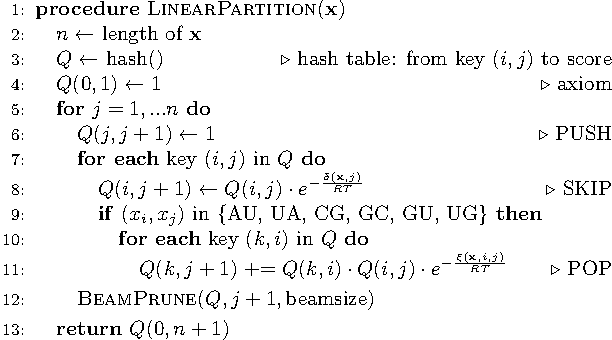
\includegraphics[scale=1]{figs/algorithm}
\caption{
LinearPartition algorithm.
\label{algorithm}}
\vspace{-0.3cm}
\end{figure*}
% } % Display the Materials and Methods section

% \vspace{-0.5cm}
% \acknow{\small 
% This work was partially supported by 
% NSF grant IIS-1817231 (L.H.) and NIH grant R01 GM076485 (D.H.M.).
% We thank Rhiju Das for the early adoption of
% our software in the EteRNA game.
% \vspace{-0.5cm}
% }

% \showacknow{} % Display the acknowledgments section
% \smallskip

% \pnasbreak splits and balances the columns before the references.
% Uncomment \pnasbreak to view the references in the PNAS-style
% If you see unexpected formatting errors, try commenting out \pnasbreak
% as it can run into problems with floats and footnotes on the final page.
%\pnasbreak

% Bibliography
\vspace{-0.6cm}
\section*{References}
\balance
% \bibliographystyle{elsarticle-harv} % can't use any; already used unsrt in pnas-new.cls
\bibliography{main}

\appendix

\newpage

% % !TEX root = linearpartition.tex

\setcounter{figure}{0}
\renewcommand{\thefigure}{Online Method \arabic{figure}}
\setcounter{table}{0}
\renewcommand{\thetable}{Online Method \arabic{table}}

\section*{Online Methods}

%We propose LinearFold,
%% LinearFold is 
%% a linear-time prediction algorithm predicting RNA
%% secondary structures.
% Our \linearfold approach is 
% presented in four steps, starting from
% the most naive but easy-to-understand exhaustive search version (Fig.~\ref{fig:method} C1), and gradually 
% build it up to 
% the linear-time version (Fig.~\ref{fig:method} C4), using a stack-top merge and beam search.

Here we first formulate the \linearfold algorithm more formally.

\subsection*{Formulation}
%% The RNA secondary structure prediction problem can be formalized as follows,
%% using the dot-bracket format to represent structures.
Generally, given an input RNA sequence
$$ \vecx = x_1x_2\ldots x_{n}, \text{ where } x_i \in \{\tt{A},\tt{C},\tt{G},\tt{U}\},$$
the RNA secondary structure prediction algorithm
%$\mathit{f}$ 
aims to find the best-scoring pseudoknot-free structure
%$$ \vecy = y_1y_2\ldots y_{n}, \text{ where } y_i \in \{\md, \ml, \mr\}$$
%(to address pseudoknots, different types of brackets would be required)
according to a scoring function \score (e.g., model score or negative free energy) parameterized by model $\weight$:
% (or minimum model cost):
\vspace{-0.1cm}
% \begin{equation}
%   %f(\vecx) =
%   \argmax_{\vecy \in \GEN(\vecx)} \score(\vecx, \vecy; \weight)
%   \label{eq:mfe}
% \end{equation}
%\vspace{-0.2cm}
where $\GEN(\vecx)$ is the set of all possible pseudoknot-free structures
\[
\GEN(\vecx) =
\big\{\vecy \in \{\md, \ml, \mr\}^n \;\mid\; \vecy \text{~is balanced in brackets}\big\}.
\]
%and %$\score$ is the cost function (i.e., free
%energy function), and
The two baselines in our study, \contrafold
and \viennarnafold, use scoring functions that are very similar  in structure, % scoring functions,
but very different in parameters 
(the former learns \vecw from data, % in which the free energy
%is not revealed,
while the latter is based on thermodynamics).

All dynamic programming-based prediction algorithms, including ours, %like previous ones, are based on dynamic programming,
require the scoring function to {\em decompose} to the scorings of smaller structures,
in order to have efficient computation.
For example, the main text (see Fig.~\ref{fig:method}) uses the simplest Nussinov-style scoring function 
that factors to each individual base pair and simply counts the number of pairs in a structure:
\begin{equation}
  \score_{\text{Nussinov}}(\vecx, \vecy; \_) = \# \pairs(\vecy) = \sum_{(i,j)\in \pairs (\vecy)} 1
  \label{eq:nussinov}
\end{equation}
where $\pairs(\vecy)$ returns the list of base pairs in \vecy, e.g.,
$\pairs(\text{``\md\ml\ml\md\mr\mr\md''}) = \{(2,6), (3,5)\}$.
Note this scoring function does not depend on any model,
but we could in principle assign different scores in \vecw for GC, AU, and GU pairs (e.g., $w_\text{GC} > w_\text{AU} > w_\text{GU}$),
and also introduce a penalty for each unpaired nucleotide ($w_\unpaired < 0$),
which we call the ``Extended Nussinov'' model:
\begin{equation}
  \score_{\text{extended}}(\vecx, \vecy; \vecw) = \sum_{(i,j)\in \pairs (\vecy)} w_{x_i x_j} +\sum_{i\in \unpaired(\vecy)} w_\unpaired
  \label{eq:extended}
\end{equation}
In reality, the actual scoring functions % $\score$ (scoring structure \vecy on input \vecx by model \vecw) can be
used by \contrafold, \rnafold, and \linearfold are more complex and they
decompose to individual loops: % as follows:
\begin{equation}
  \begin{split}
 \score_\text{real}(\vecx, \vecy; \weight) = &
 \!\!\!\!\sum_{h \in \text{hairpin\_loops}(\vecy)}\!\!\!\! \score^{\mathrm H}(\vecx, h; \weight)  + \!\!\!\!\sum_{s \in \text{single\_loops}(\vecy)}\!\!\!\! \score^{\mathrm S}(\vecx, s; \weight) \\
 + & \!\!\!\!\sum_{m \in \text{multi\_loops}(\vecy)}\!\!\!\! \score^{\mathrm M}(\vecx, m; \weight) +  \!\!\!\!\sum_{e \in \text{external\_loops}(\vecy)}\!\!\!\!\!\!\!\! \score^{\mathrm E}(\vecx, e; \weight).
\end{split}
\label{eq:decomp}
\end{equation}
The thermodynamic %minimal free energy
model in \viennarna scores %, the score of constructing 
each type of loop %(hairpin, single-branch, multi-branch, and external)
using several feature templates such as
hairpin/bulge/internal loop lengths,
terminal mismatches, helix stacking, helix closing, etc.
%% %the following feature components:\cite{mathews+:1999}
%% \begin{itemize}[itemsep=-1mm]
%% \item %$\score^{\mathrm H}(\cdot,\cdot;\cdot)$,
%% Hairpin loops: hairpin length, terminal mismatch, and special tri-, tetra-, and hexa-loops. 
%% \item %$\score^{\mathrm S}(\cdot,\cdot;\cdot)$,
%% Single-branch loops (including helix stacking as empty loop, and bulge and internal loops):
%% bulge length, internal loop length, internal loop left-right balancing,
%% terminal mismatch, helix stacking, and helix closing.
%% \item %$\score^{\mathrm M}(\cdot,\cdot;\cdot)$,
%% Multi-branch loops: multi-loop base cost, terminal mismatch,
%% left/right dangles, multi paired, and multi unpaired.
%% \item %$\score^{\mathrm E}(\cdot,\cdot;\cdot)$,
%% External loops: left/right dangles, external paired and external  unpaired. 
%% \end{itemize}
The machine-learned model in \contrafold
replaces energies in the above framework with model weights learned from data.
%all the model weights are learned from data, instead of the free energy.
%% We conclude
%% the cost decomposition in Fig.~\ref{fig:realdeduct}. 

%% RNA secondary structure prediction is regarded as a challenging problem,
%% that no existing model can score perfectly to match the actual
%% structure with the minimum free energy (or minimum model cost) function, i.e.,
%% {\bf imperfect modeling}.
%% Consider $y^*(\vecx)$ as the actual secondary structure of the given sequence,
%% and an evaluation metric (e.g., PPV, sensitivity) $M$ to
%% calculate accuracy of a set of predicted structures against the actual
%% structures ($M(y,y)=1$), we are likely to have $M(f(\vecx), y^*(\vecx)) < 1$
%% according to the existing results reported(see Fig.\ref{fig:accuracy}).

%% Our proposed \linearfold algorithm can linearize any system with a variant of
%% $(\score,\weight)$, as long as $f(\vecx) = \argmin_{\vecy \in \GEN(\vecx)}
%% \score(\vecx, \vecy; \weight)$ can be 
%% solved in cubic-time by the dynamic programming algorithm.
%% The linearization maintains the same cost function and model $(\score,\weight)$,
%% but the objective function is different, i.e. $f' \neq f$, as we set a series of
%% soft constraints
%% during the beam search, pruning out structures with high cost or high free
%% energy which depends on the given $(\score,\weight)$.
%% Experimental results show that
%% this difference leads to a higher accuracy in linearizing \contrafold and
%% Vienna RNAfold (see Fig.~\ref{fig:accuracy} and Fig.~\ref{fig:beamsize}).

Our \linearfold algorithm can ``linearize'' any cubic-time prediction system
as long as the scoring function decomposes in a way similar to Eqs.~\ref{eq:nussinov}--\ref{eq:decomp} above.
Below we formalize our \linearfold algorithm step by step, % as follows.
using the Extended Nussinov model in Eq.~\ref{eq:extended} to strike a balance between simplicity
and reality.
We will refer to both the high-level illustration in Fig.~\ref{fig:method},
and a more formal deductive system in Fig.~\ref{fig:deduction}.

% The basic idea of our proposed

% We propose \linearfold, the first global linear-time RNA secondary structure
% prediction algorithm. 
% The basic idea of linear-time prediction is to predict incrementally from
% left to right,
% %, inspired by human sentence processing. To adapt it to RNA
% %sequences, 
% %we view the problem as incrementally converting the RNA sequence into
% %the dot-bracket format, such that 
% labeling each nucleotide  as unpaired ``{\textbf .}'', opening ``{\textbf (}'',
% or closing ``{\textbf )}''. 
% %% This makes the
% %% dot-bracket format equivalent to the pseudoknot-free RNA secondary structures
% We require this dot-bracket string to be well-balanced as we only consider pseudoknot-free structures
% (to address pseudoknots, different types of brackets would be required. This is left as our future work). 

% the term "exponentially traverse" is strange, I suggest "traverse all possible
% structures in GEN(\vecx), which takes exponenential time
%% 4-step method claim
%\vspace{.25cm}
\subsection*{Naive exhaustive incremental prediction: $O(3^n)$ time}
By exhaustively predicting $y$ from left-to-right, we
traverse all the possible structures in $\GEN(\vecx)$,
% calculate the free energy for each of them,
and pick the one with the highest score (or lowest free energy). % or model cost.
We denote each {\em state} at step $j$ ($j \in \{0,\ldots, n\}$)
as a tuple along with a score $s$:
%\begin{equation}
\[
        \nnitem{\vecy}{\sigma}{j}{s},
\]
%$s = \nitem{{\bm \sigma} | i}{j}\vecy$,
%\end{equation}
where \vecy is the (sub)structure for the prefix $x_1 \ldots x_j$,
and
$\sigma$ is the  stack consisting of unmatched opening bracket positions in \vecy.
For the Nussinov model, score $s$ is simply the number of pairs in \vecy.
For example, if \vecy=``\md\ml\ml\md\mr\ml'', then $\sigma=[2,6]$ and $s=1$.
%and $s$ is the score of the state.
%% so far
%% where $i$ is the top of the stack, meaning $x_i$ is the last unmatched opening nucleotide. 
%$\vecy$ is the corresponding dot-bracket (sub)sequence up to $x_{j-1}$.
Each state can transition into a subsequent state, taking one of the three
actions:
\begin{enumerate}
\itemsep-0.2em
\item \push:
$\nnitem{\vecy}{\sigma}{j}{s} \goesto \nnitem{\vecy\!\circ\!{\text `}\ml{\text '}}{\sigma | j}{j+1}{s}$.
%which labels the current nucleotide $x_j$ as a left bracket ``{\textbf (}'', 
%putting it on top of the stack;
\item \nskip:
$\nnitem{\vecy}{\sigma}{j}{s} \goesto \nnitem{\vecy\!\circ\!{\text `}\md{\text '}}{\sigma}{j+1}{s + w_\unpaired}$.
%, which labels $x_j$ as a dot ``{\textbf .}'', leaving the stack unchanged,
%and 
\item \pop:
$\nnitem{\vecy}{\sigma | i}{j}{s} \goesto \nnitem{\vecy\!\circ\!{\text `}\mr{\text '}}{\sigma}{j+1}{s+ w_{x_i, x_j}}$
(if $x_i$ and $x_j$ can form a base pair).
%, which labels $x_j$ as a right bracket ``{\textbf )}'', 
%if it matches $x_i$
%nucleotide with $x_{\TOP}$, the top of the stack, 
%and popping $i$ from the stack.
\end{enumerate}
See Fig.~\ref{fig:deduction}(a) for the deductive system.
% labeled dot-bracket sequences ($|y|=j$).
% Then the prediction algorithm
% starts with \(\nitem{\sigma_{\epsilon}}{0}{\epsilon}\), and ends with
% $|\GEN(x)|$ different states,
% \begin{equation}
%   \nitem{\sigma_{\epsilon}}{n}{y} ,y \in \GEN(x).
% \end{equation}
%% Starting at the state \(\nitem{\sigma_{\epsilon}}{0}{\epsilon}\), it takes
This algorithm takes $O(3^n)$ time to exhaustively traverse all possible
%structures (see the first part of Figure~\ref{fig:method}).
structures (see Figure~\ref{fig:method}D1).

% we start with an empty structure, with the current
% index at the beginning of the sequence, 
% The algorithm is
% with $O(3^n)$ time. 

% the structure $y \in \GEN(x)$ satisfies $y =y_1y_2...y_n, y_i \in \{\textbf{. (
%   )}\}$, with a balanced of brackets. We note $\pair(y) = \{(i,j) | (y_i,y_j)
% \text{~matches~in~brackets}\}$. 

% Now, given an free energy function
% $\energy$ and a model $\weight$ , our algorithm is to find the structure with
% the minimum free energy,

% we view the problem as incrementally converting the RNA sequence into the
% dot-bracket format, that each nucleotide can be labeled as unpaired ``{\tt .}'' (a
% skip action), opening ``{\tt (}'' (a push action), or closing ``{\tt )}'' (a pop
% action). The naive exhaustive prediction method would seem to require $O(3^n)$
% time, as there are 3 different labels for each nucleotide.

%\vspace{.25cm}
\subsection*{Dynamic Programming via Identical-Stack Merging:
  $O(2^{n})$ time}

Now we apply dynamic programming on top of this exhaustive method to exploit
shared computations.
Consider a simple case that two states can be merged: if
there are two states in the same step $j$,
% $\nitem{\bm \sigma}{j}\vecy$ and $\nitem{\bm \sigma}{j}{\vecy'}$, 
% sharing the exact same stack $\bm \sigma$ but with different dot-bracket strings $\vecy$ and $\vecy'$, 
%i.e.,
%they have the same positions of all unpaired openings %, means that they have identical stacks, 
we say that these two states are ``equivalent'' and we can merge them
(and only keep the better scoring between \vecy and $\vecy'$). 
%A merged state can be represented as $\twotuple{\bm \sigma}{j}$. 
Fig.~\ref{fig:method}B(Idea 1)/D2 illustrates this merging and
Fig.~\ref{fig:deduction}(b) shows the deductive system. 
Although we merge to reduce the number of states, it is still exponential time, 
% use fewer states to process, the number of
% possible states are still exponential,
since there could be exponentially many
different stacks in each step. 
% against the current index $j$.
This algorithm takes $O(2^{n})$ time. 
%%  for every possible stack
%% $\twotuple{\bm \sigma}{j}$ considered in the prediction process.

%\vspace{.25cm}
\subsection*{Dynamic Programming via Stack Top Packing: $O(n^3)$ time}

To avoid considering exponentially many states, 
we further
%% further apply the
%% Graph-Structured Stack (GSS, \cite{Tomita:1988}) to the dynamic programming. 
pack states with different stacks.
Consider two states in the same step $j$,
% $\twotuple{{\bm \sigma_0} | i}{j}$ and $\twotuple{{\bm \sigma_1} | i}{j}$,
which share the last unpaired opening $i$ (i.e., stack top). 
%(where $i$ is the same top of the stack).
We call these states ``temporarily equivalent'', since they can be treated as
exactly the same until the unpaired opening $x_i$ is closed (and thus popped from the stack).
% In other words we can represent both stacks ${\bm \sigma_0} | i $ and ${\bm \sigma_1} | i$
as $...i$, where $...$ denotes part of the history that we do not need at this moment.
This factorization of stacks is called ``Graph-Structured Stacks'' (GSS) by Tomita. \cite{Tomita:1988}
After packing, we define the new state to be $\tuple{i,j}$
%In our dynamic programming prediction algorithm, 
and therefore we  maintain $O(n^2)$ states.
For each state $\tuple{i,j}$, the pop action
can take worst-case $O(n)$ time because $\tuple{i,j}$ can combine with every $\tuple{k,i}$ from step $i$.
%due to the graph-structured stack. 
Thus the overall time complexity is $O(n^3)$.
See Fig.~\ref{fig:method}B(Idea 2)/D3 for  
an example of the packing process
and Fig.~\ref{fig:deduction}(c,d)
for the deductive system.

Now we explain the
packing on these ``temporarily equivalent'' states in detail. 
We use the GSS \cite{Tomita:1988} to pack and unpack
them, which has been widely used in parsing natural language sentences.
\cite{huang+sagae:2010}
% The idea is to combine
The idea behind the packing process is to combine the left structure information
of different states packed together in the push action,
and this structure is later unpacked in the future pop action.

Basically, if state $r$ generates state $s$ by a push action, then $r$ is added
onto $\pi(s)$, a set of predictor states. When two equivalent pushed states get
packed, we combine their predictor states. For example, if $r_x =
\tuple{t_x, j}$ predicts $s = \tuple{j,j+1}$ for $x\in \{0,\ldots, k\}$, then $\pi(s) =
\{r_x|x=0 \ldots k\}$. 
% In the pop step, state $s = \tuple{i,j}$ tries to combine with every predictor
% state $r \in \pi(s)$, and the resulting state $t$ inherits the predictor states
% set from $r$, i.e., $\pi(t) = \pi(r)$. 
To pop state $s = \tuple{i,j}$, we combine it with each of its predictor states
$r \in \pi(s)$ to make a resulting state $t$.
$t$ inherits the predictor states from $r$, i.e., $\pi(t) = \pi(r)$.

% We further merge them together since they can be treated as
% exactly same state until the unpaired opening $i$ has
% been closed. In other words, these two states are ``temporarily equivalent''.
% Although they are not equivalent states, comparing to the full-stack merge, the
% computation of these two states are with no difference before the last unpaired
% openings has been closed.
% An example of the merged prediction process is shown in Figure~\ref{fig:method}. 

Moreover, the empirical running time of our algorithm is better than cubic.
As we restrict only three types of allowed pairs ({\tt AU}, {\tt CG},
{\tt GU}) in the prediction, the pop action happens only if $(x_i, x_{j+1})$ is
one of the allowed pairs. Thus, in the skip action, we can skip nucleotides
until the next one $x_{j+1}$ can be paired with $x_i$.
We observe this emperical running time is approximately $O(n^{2.6})$, similar to
previous bottom-up dynamic programming methods.\cite{do+:2006,
  lorenz+:2011, mathews+turner:2006}

%% Similar to previous methods, we avoid sharp turns as well. All base-pairs in the
%% predicted RNA secondary structures must be with a distance $\geq 4$. 

% There is a no-sharp-turn setting in the previous methods as well, that all
% base-pairs in the predicted RNA secondary structure must be with a distance
% $\geq 4$ nucleotides, so that sharp turns in the RNA secondary structure are
% avoided.

%\vspace{.25cm}
\subsection*{Dynamic Programming via Beam Search: $O(n)$ time}
Although our stack-top packing version still runs cubically, the same as the
conventional baselines, 
 this left-to-right search is easily ``linearizable'' 
unlike the bottom-up CKY-based algorithms used by most of the existing systems for RNA structure prediction.
%, especially with long sequences.
% with a rich feature set in the RNA secondary structure prediction
% problem.
We further employ beam search pruning \cite{huang+:2012} 
to reduce the complexity to linear time.
% Thus we extend it with a beam search framework.
%% need or not?
% Although our dynamic programming algorithm is the of same complexity as 
% traditional algorithms, the key difference is that our new dynamic programming
% algorithm is {\bf incremental} (i.e., left-to-right) instead of  {\bf
%   bottom-up} as in traditional CKY-style algorithms (Nussinov, Zuker, McCaskill,
% etc.), which makes the beam search framework only applicable to our prediction algorithm.
Generally, we only keep the $b$ top-scoring (low-energy) states $\tuple{i, j}$ 
%by score 
for each step $j$. In this way all the lower-scoring (high-energy) states are pruned
out, and if a
structure survives to the end, it must have been one of the top $b$
states in every step.
This pruning also means that in a pop action, a state $(i,j)$ can combine with at most $b$ states $(k,i)$ from step $i$.
Thus the overall time complexity is $O(nb^2)$.
%% , i.e., a pop
%% action can produce at most $b$ subsequent states.
However, instead of generating $b^2$ new states from a pop action, % from a step $j$, 
we use \textbf{cube pruning} \cite{huang+chiang:2007} to generate the best
$b$ states, which would take $O(b\log b)$ time.
Thus the overall running time over a length-$n$ sequence is $O(nb\log b)$, see 
See Figure~\ref{fig:method}C(Idea 3)/D4 for beam search.

% Generally,
%at each step, we choose the best $b$ resulting states from all the
%merged states in this step, and use these states only for the next steps. For
% for all the merged states $\tuple{i, j}$ sharing the same $j$,
% we cut to top $b$ by their scores so far.

% Moreover, we can further improve the time complexity of the pop actions, by
% considering all of them at once using \textbf{cube
%   pruning}\cite{huang+chiang:2007}. 
% % the time complexity of the pop actions could be further improved.
% Assume we have $b$ states in step $j$, each which contain at most $b$ left
% pointers. 
% Instead of generating $b^2$ new states from their pop actions,
% We use cube pruning to generate the best
% $b$ states. This would take $O(b\log(b))$ time. 

 
% $b'$ of them can lead to a pop action
% towards the next step $j+1$, and each of them contains $b$ left pointers. 

% In the pop action of the GSS, 

% Moreover, for each step, 

% since $b$ states are maintained in each step, our pop action, 


% This beam pruning guarantees our algorithm costs a constant amount of time at
% each step, thus our prediction algorithm is linear-time overall.

% As a result, it is fairly easy to apply beam search pruning (a common search technique
% in Artificial Intelligence, see for example \cite{zhang+clark:2008}) 
   %    on top of our left-to-right algoithm,
% where we allow at most $b$ top-scoring states to survive in each step
% ($b$ is a constant called ``beam width'').
% Those lower-scoring states that do not make the cut are deemed unpromising,
% and it is unlikely (though possible) that those pruned states 
% would lead to the best result in the end.
% So beam search reduces the runtime to $O(n)$ at the cost of minor search errors.
% By contrast, applying the same pruning idea to the traditional bottom-up algorithm
% will still result in $O(n^3)$ time because the pruning here is per $[i,j]$ span 
% instead of per step $j$.

\iffalse
\subsection*{Incorporating Models}
"To directly compare our approach with previous work, \linearfoldv is
based on the thermodynamic \viennarnafold model \cite{lorenz+:2011} and uses all
of the exact same features. Similarly, 
  \linearfoldc is based on the machine learned \contrafold model \cite{do+:2006}
with all of its same features. This is so that without beam search, {\em
  LinearFold} will produce exactly the same predictions. 

We also observe the difference between these two types of models. More details
are provided in the Supplementary Information (SI). 
\fi

%\vspace{.25cm}
\subsection*{Dataset, Evaluation Metrics and Significance Testing}\label{dataset}
We choose the ArchiveII dataset, \cite{sloma+mathews:2016}
a diverse set of over 3,000 RNA sequences with known secondary structures.
But since the current \contrafold machine-learned model (v2.02) is trained on the S-Processed dataset \cite{andronescu+:2007}
%\footnote{\url{http://www.rnasoft.ca/CG/}}, 
we removed those sequences that appeared in the S-Processed dataset. 
The resulting dataset we used contains 2,889 sequences over 9 families, with an average length of 222.2 \nts. 

We use a sampled subset of RNAcentral to test our efficiency and scalability
performance. For the sampling, we evenly split the range from $1,000$ to
$244,296~$(the longest sequence) into 30 bins by log-scale, and for each bin we
randomly select up to $10$ sequences from the original data (there are bins with
$0$ or $1$ sequence only).
For each bin, we take the average over all sequences
and report the averaged time and memory cost. 

% from the ArchiveII dataset that are also found in the S-Processed set
% to have a clear separation between training and testing sets.
% Following \cite{sloma+mathews:2016}, we also removed the Group II Intron family.
%% the RNA sequences in the Mathews dataset that shares with the
%% S-Processed dataset.
%% We've also removed the Group II Intron family, according to the dataset
%% author.?

Due to the uncertainty of base-pair matches existing in comparative analysis
and the fact that there is fluctuation in base pairing at equilibrium,
we
consider a base pair to be correctly predicted if it is also displaced by one
nucleotide on a strand.\cite{sloma+mathews:2016}
Generally, if a pair $(i,j)$ is in the predicted structure, we consider it a
correct prediction if one of $(i,j)$, $(i-1,j)$, $(i+1,j)$, $(i,j-1)$, $(i,j+1)$ is in the
ground truth structure.
We also report the accuracy using exact base pair matching instead of this
method, in Figure~\ref{tab:accuracy_nos}. 
%To evaluate the accuracy, 
Both sensitivity and PPV are reported.
%Positive Predictive Value
%(PPV), 
Generally, if $\vecy$ is the predicted structure and $\vecy*$ is the ground
truth, we have
$$ \sens = \frac{\text{true positives}}{\text{true positives} +
  \text{false negatives}} =
\frac{|\vecy \cap \vecy^*|}{|\vecy^*|},$$
$$\ppv = \frac{\text{true positives}}{\text{true positives} +
  \text{false positives}} = \frac{|\vecy \cap \vecy^*|}{|\vecy|}. $$
For the statistical significance test, 
we use the paired two-tailed $t$-test to check the statistical significance,
with the type I error rate set to $0.05$,
consistent with the previous methods. \cite{xu+:2011}
%% \cite{sloma+mathews:2016}. 



\begin{figure*}[b]
\center
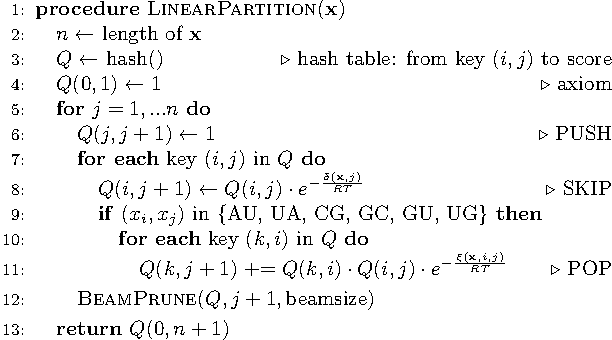
\includegraphics[scale=1]{figs/algorithm}
\caption{
LinearPartition algorithm.
\label{algorithm}}
\vspace{-0.3cm}
\end{figure*}

% !TEX root = main.tex
\onecolumn
\newpage


%\begin{titlepage}
  \begin{centering}
    \vspace*{1cm}
    
    \textbf{\Large Supporting Information}\\
    \vspace{0.5cm}
    \textbf{\Large \linearpartition: Linear-Time Approximation of RNA Folding Partition Function and Base Pairing Probabilities}\\
    \vspace{0.5cm}
    \textbf{\large
    He Zhang, Liang Zhang, David H.~Mathews and Liang Huang}
    \vspace{1.5cm}
    
  \end{centering}
%\end{titlepage}

\setcounter{figure}{0}
\renewcommand{\thefigure}{SI\,\arabic{figure}} % spacing
\setcounter{table}{0}
\renewcommand{\thetable}{SI\,\arabic{table}}
\setcounter{page}{1}
% \renewcommand{\thepage}{\arabic{chapter}.\arabic{page}} 

\setcounter{section}{0}
\renewcommand\thesection{\Alph{section}}
\setcounter{subsection}{0}
\renewcommand\thesubsection{\Alph{section}.\arabic{subsection}}

% \setcounter{reference}{0}


\section{Details of the Efficient Implementation}
\label{sec:si:algdetails}

\titleformat{\subsection}%[runin]
{\normalfont\bfseries}% formatting commands to apply to the whole heading
        {\thesubsection}% the label and number
        {0.5em}% space between label/number and subsection title
        {#1}% formatting commands applied just to subsection title
        []
        
\subsection{Data Structures}

%\begin{table}
In the main text, for simplicity of presentation, $Q$ is described as a hash from span $[i,j]$
to $\Qf{i}{j}$, but in our actual implementation,
to make sure the overall runtime is $O(n b^2)$,  we implement $Q$ as
an array of $n$ hashes, where each $Q[j]$ is a hash
mapping $i$ to $Q[j][i]$ which is conveniently notated as \Qf{i}{j} in the main text. It is important to note that the first dimension $j$ is the right boundary
and the second dimension $i$ is the left boundary of the span $[i,j]$. See the following table for a summary of notations and the corresponding actual implementations.
Here we use Python notation for simplicity, but in actual system we implement with C++.
\begin{center}
%\resizebox{0.5\textwidth}{!}{
\begin{tabular}{l|l}
notations in this paper & Python implementation\\
\hline
%$Q\gets$ hash() & \verb|Q = defaultdict(lambda : defaultdict(float))|\\
$Q\gets$ hash() & {\tt Q = [defaultdict(float) \textbf{for} \_ \textbf{in} range(n)]}\\
\Qf{i}{j} & \verb|Q[j][i]| \\
$[i,j]$ in $Q$ & {\tt i \textbf{in} Q[j]}\\
{\bf for each} $i$ such that $[i,j]$ in $Q$ & {\tt \textbf{for} i \textbf{in} Q[j]}\\
{\bf delete} $[i,j]$ from $Q$ & {\tt \textbf{del} Q[j][i]}
\end{tabular}
%}
\end{center}
%\end{table}

\subsection{Complexity Analysis}

In the partition function calculation (inside phase) in Fig.~\ref{fig:algorithm},
the number of states is $O(nb)$ because each $Q[j]$ contains at most $b$ states (\Qf{i}{j}'s) after pruning. Therefore the space complexity is $O(nb)$.
For time complexity, there are three nested loops, the first one ($j$) with $n$ iterations,
the second ($i$) and the third ($k$) loops both have $O(b)$ iterations thanks to pruning, so the overall runtime is $O(nb^2)$.

\subsection{Outside Partition Function and Base Pairing Probability Calculation}
\label{sec:outside}

After we compute the partition functions \Qf{i}{j} on each span $[i,j]$ (known as the ``inside partition function''),
we also need to compute the complementary function \Qhatf{i}{j} for each span known as
the ``outside partition function'' in order to derive the base-pairing probabilities. 
Unlike the inside phase, this outside partition function is calculated from top down,
with $\Qhatf{1}{n} = 1$ as the base case.
\begin{equation*}
\begin{split}
\Qhatf{i}{j} & = \Qhatf{i}{j+1} \cdot e^{-\frac{\delta(\vecx, j+1)}{RT}} \\
                  & + \sum_{k < i} \Qhatf{k}{j+1} \cdot \Qf{k}{i-2} \cdot e^{-\frac{\xi(\vecx,i-1,j+1)}{RT}} \\
                  & + \sum_{k > j+1} \Qhatf{i}{k} \cdot \Qf{j+2}{k-1} \cdot e^{-\frac{\xi(\vecx,j+1,k)}{RT}}
\end{split}
\end{equation*}
Note that the second line is only possible when $x_{i-1} x_{j+1}$ can form a base pair
(otherwise $e^{-\frac{\xi(\vecx,i-1,j+1)}{RT}} = 0$)
and the third line has a constraint that $x_{j+1}x_k$ can form a base pair 
(otherwise $e^{-\frac{\xi(\vecx,j+1,k)}{RT}} = 0$).


For each $(i,j)$  where $x_i x_j$ can form a base pair, we compute its pairing probability:
\[
p_{i,j}  = \sum_{k \leq i} \Qhatf{k}{j} \cdot \Qf{k}{i-1} \cdot e^{-\frac{\xi(\vecx,i,j)}{RT}} \cdot \Qf{i+1}{j-1}
\]

The whole ``outside'' computation takes $O(n^3)$ without pruning,
but also $O(nb^2)$ with beam pruning.
See Fig.~\ref{fig:outside} for the pseudocode to compute the outside partition function and base pairing probabilities.

%\subsection{Supporting Pseudocode}

\section{Details of datasets, baselines and methods}

% \newpage
\subsection{Datasets}
\label{sec:datasets}

We use sequences from two datasets, ArchiveII and RNAcentral.
The archiveII dataset 
(available in \url{http://rna.urmc.rochester.edu/pub/archiveII.tar.gz}) is % \cite{sloma+mathews:2016}, 
a diverse set with 3,857 RNA sequences and their secondary structures.
It is first curated in the 1990s to contain sequences with structures that were well-determined by comparative sequence analysis~\cite{mathews+:1999}% [72] 
and updated later with additional structures~\cite{sloma+mathews:2016}. % [96].  
% and is available in \url{http://rna.urmc.rochester.edu/pub/archiveII.tar.gz}.
We remove 957 sequences that appear both in the ArchiveII and the S-Processed datasets~\cite{Andronescu+:2007}, 
because CONTRAfold uses S-Processed for training. 
We also remove all 11 Group II Intron sequences 
because there are so few instances of these that are available electronically.
Additionally, we removed 30 sequences in the tmRNA family because the annotated structure for each of these sequences contains fewer than 4 pseudoknots, 
which suggests the structures are incomplete. 
These preprocessing steps lead to a subset of ArchiveII with 2,859 reliable secondary structure 
% RNA sequence and structure pairs 
examples 
distributed in 9 families. 
See~\ref{tab:archiveII} for the statistics of the sequences we use in the ArchiveII dataset.
% But since CONTRAfold (v2.02) machine-learned model is trained on the S-Processed dataset \cite{},
% we removed those overlap sequences. 
% As in \linearfold paper, we also remove those sequences CONTRAfold (v2.02) used for training.
% The remaining dataset contains 2889 RNA sequences from 9 families, 
% with average length 222 $nt$ and max length 2968 $nt$.
Moreover, we randomly sampled 22 longer RNA sequences (without known structures) from RNAcentral~\cite{rnacentral:2017} 
% (The RNAcentral Consortium, 2017) 
(\url{https://rnacentral.org/}),
with sequence lengths ranging from 3,048~{\it nt} to 244,296~{\it nt}.
For the sampling, we evenly split the range from $3,000$ to $244,296$ (the longest) into 24 bins by log-scale, and for each bin we
randomly select a sequence (there are bins with
no sequences).
% (Homo Sapiens Transcript NONHSAT168677.1, from the NONCODE database (Zhao et al., 2016)).
% We run all experiments 
% % (compiled by GCC 4.9.0) 
% on a Linux machine, 
% with 2.90GHz Intel Core i9-7920X CPU and 64G memory.

To show the approximation quality on random RNA sequences, 
we generated 30 sequences with uniform distribution over \{A, C, G, U\}.
% The lengths of these sequences are 100, 200, ..., 3000.
The lengths of these sequences are spaced in 100 nucleotide intervals from 100 to 3,000.
% with lengths range from 100~{\it nt} to 3,000~{\it nt}. 


\begin{table}[!h] % hzhang: redo with new data
  \centering
  \large
  \setlength{\tabcolsep}{12pt}
  \begin{tabular}{r|rr|rrr}
    & \multicolumn{2}{c|}{\# of seqs} & \multicolumn{3}{c}{length} \\
    Family & total & used & avg & max & min \\
    \hline
    tRNA  & 557 & 74  & 77.3  & 88 &58  \\
    5S rRNA & 1,283 & 1,125 & 118.8 & 135 &102  \\
    SRP RNA & 928 & 886 & 186.1 & 533 & 28\\
    RNase P RNA & 454 & 182 & 344.1 & 486 & 120 \\
    tmRNA & 462 & 432 & 369.1 & 433 & 307 \\
    Group I Intron  & 98  & 96  & 424.9 & 736 &210  \\
    Group II Intron  & 11  & 0  & - & -&-  \\
    telomerase RNA  & 37  & 37  & 444.6 & 559 &382\\
    16S rRNA  & 22  & 22  & 1,547.9  & 1995 & 950\\
    23S rRNA  & 5 & 5 & 2,927.4  & 2968& 2904\\
    \hline
    {\em Overall} & 3,846 & 2,859 & 221.1 &2968 &28 \\
  \end{tabular}
  \\[0.3cm]
  % \smallskip
  \caption{Statistics of the sequences in the ArchiveII dataset used in this work.
    \label{tab:archiveII}}
\end{table}


\subsection{Baseline Software}

We use two baseline software packages: 
(1) \viennarnafold %~\cite{lorenz+:2011}
(Version 2.4.11) 
from 
\url{https://www.tbi.univie.ac.at/RNA/download/sourcecode/2_ 4_x/ViennaRNA-2.4.11.tar.gz} 
and 
(2) \contrafold %~\cite{do+:2006}
(Version 2.0.2) 
from
\url{http://contra.stanford.edu/}.
\viennarnafold is a widely-used RNA structure prediction package,
while \contrafold is a successful machine learning-based RNA structure prediction system.
Both provide partition function and base pairing probability calculations based on 
the classical cubic runtime algorithm.
Our comparisons mainly focus on the systems with the same model, 
i.e., \linearpartitionv vs. \viennarnafold and \linearpartitionc vs. \contrafold.
In this way the differences are based on algorithms themselves rather than models.
% bugs in contrafold
We found a bug in \contrafold by comparing our results to CONTRAfold, 
which led to overcounting multiloops in the partition function calculation.
We corrected the bug, and all experiments are based on this bug-fixed version of \contrafold.


\subsection{Evaluation Metrics and Significance Test}

Due to the uncertainty of base-pair matches existing in comparative analysis
and the fact that there is fluctuation in base pairing at equilibrium,
we consider a base pair to be correctly predicted if it is also displaced by one
nucleotide on a strand~\cite{mathews+:1999}.
Generally, if a pair $(i,j)$ is in the predicted structure, we consider it a
correct prediction if one of $(i,j)$, $(i-1,j)$, $(i+1,j)$, $(i,j-1)$, $(i,j+1)$ is in the
ground truth structure.
% We also report the accuracy using exact base pair matching instead of this
% method, in Figure~\ref{tab:accuracy_nos}. 
%To evaluate the accuracy, 
% Both sensitivity and PPV are reported.
%Positive Predictive Value
%(PPV), 

We use Positive Predictive Value (PPV)
and sensitivity 
as accuracy measurements. 
Formally, denote $\vecy$ as the predicted structure and $\vecy^{*}$ as the ground
truth, we have:
% $\ppv = \frac{\text{true positives}}{\text{true positives} +
%   \text{false positives}} = \frac{|\vecy \cap \vecy^*|}{|\vecy|} $
% $ \sens = \frac{\text{true positives}}{\text{true positives} +
%   \text{false negatives}} =
% \frac{|\vecy \cap \vecy^*|}{|\vecy^*|}$

$$\ppv = \frac{\#_{\text {TP}}}{\#_{\text {TP}} + \#_{\text {FP}}}  = 
\frac{|\pairs(\vecy) \cap \pairs(\vecy^*)|}{|\pairs(\vecy)|} $$

$$ \sens = \frac{\#_{\text {TP}}}{\#_{\text {TP}} + \#_{\text {FN}}}  =
\frac{|\pairs(\vecy) \cap \pairs(\vecy^*)|}{|\pairs(\vecy^*)|}$$
where $\#_{\text {TP}}$ is the number of true positives (correctly predicted pairs),
$\#_{\text {FP}}$ is the number of false positives (wrong predicted pairs)
and $\#_{\text {FN}}$ is the number of false negatives (missing ground truth pairs).

We test statistical significance using a paired, two-sided permutation test~\cite{Aghaeepour+Hoos:2013}.
We follow the common practice, choosing $10,000$ as the repetition number
and $\alpha=0.05$ as the significance threshold.
% following previous work~\cite{Aghaeepour+Hoos:2013}.

\subsection{Curve Fitting}
We determine the best exponent $a$ for the scaling curve $O(n^a)$ for each data series in Figures~\ref{fig:linearpairs} and \ref{fig:runtime}.
Specifically, we use $f(x) = a x + b$ to fit the log-log plot of those series in Gnuplot;
e.g., fitting $\log t_n = a \log n + b$, where $t_n$ is the running time on a sequence of length $n$,
so that $t_n = e^b n^a$.
Gnuplot uses the nonlinear least-squares Marquardt-Levenberg algorithm.


\newpage
\section{Supporting Figures}

\begin{figure}[h]%[b]
\center
\small
% \hspace{-0.23cm}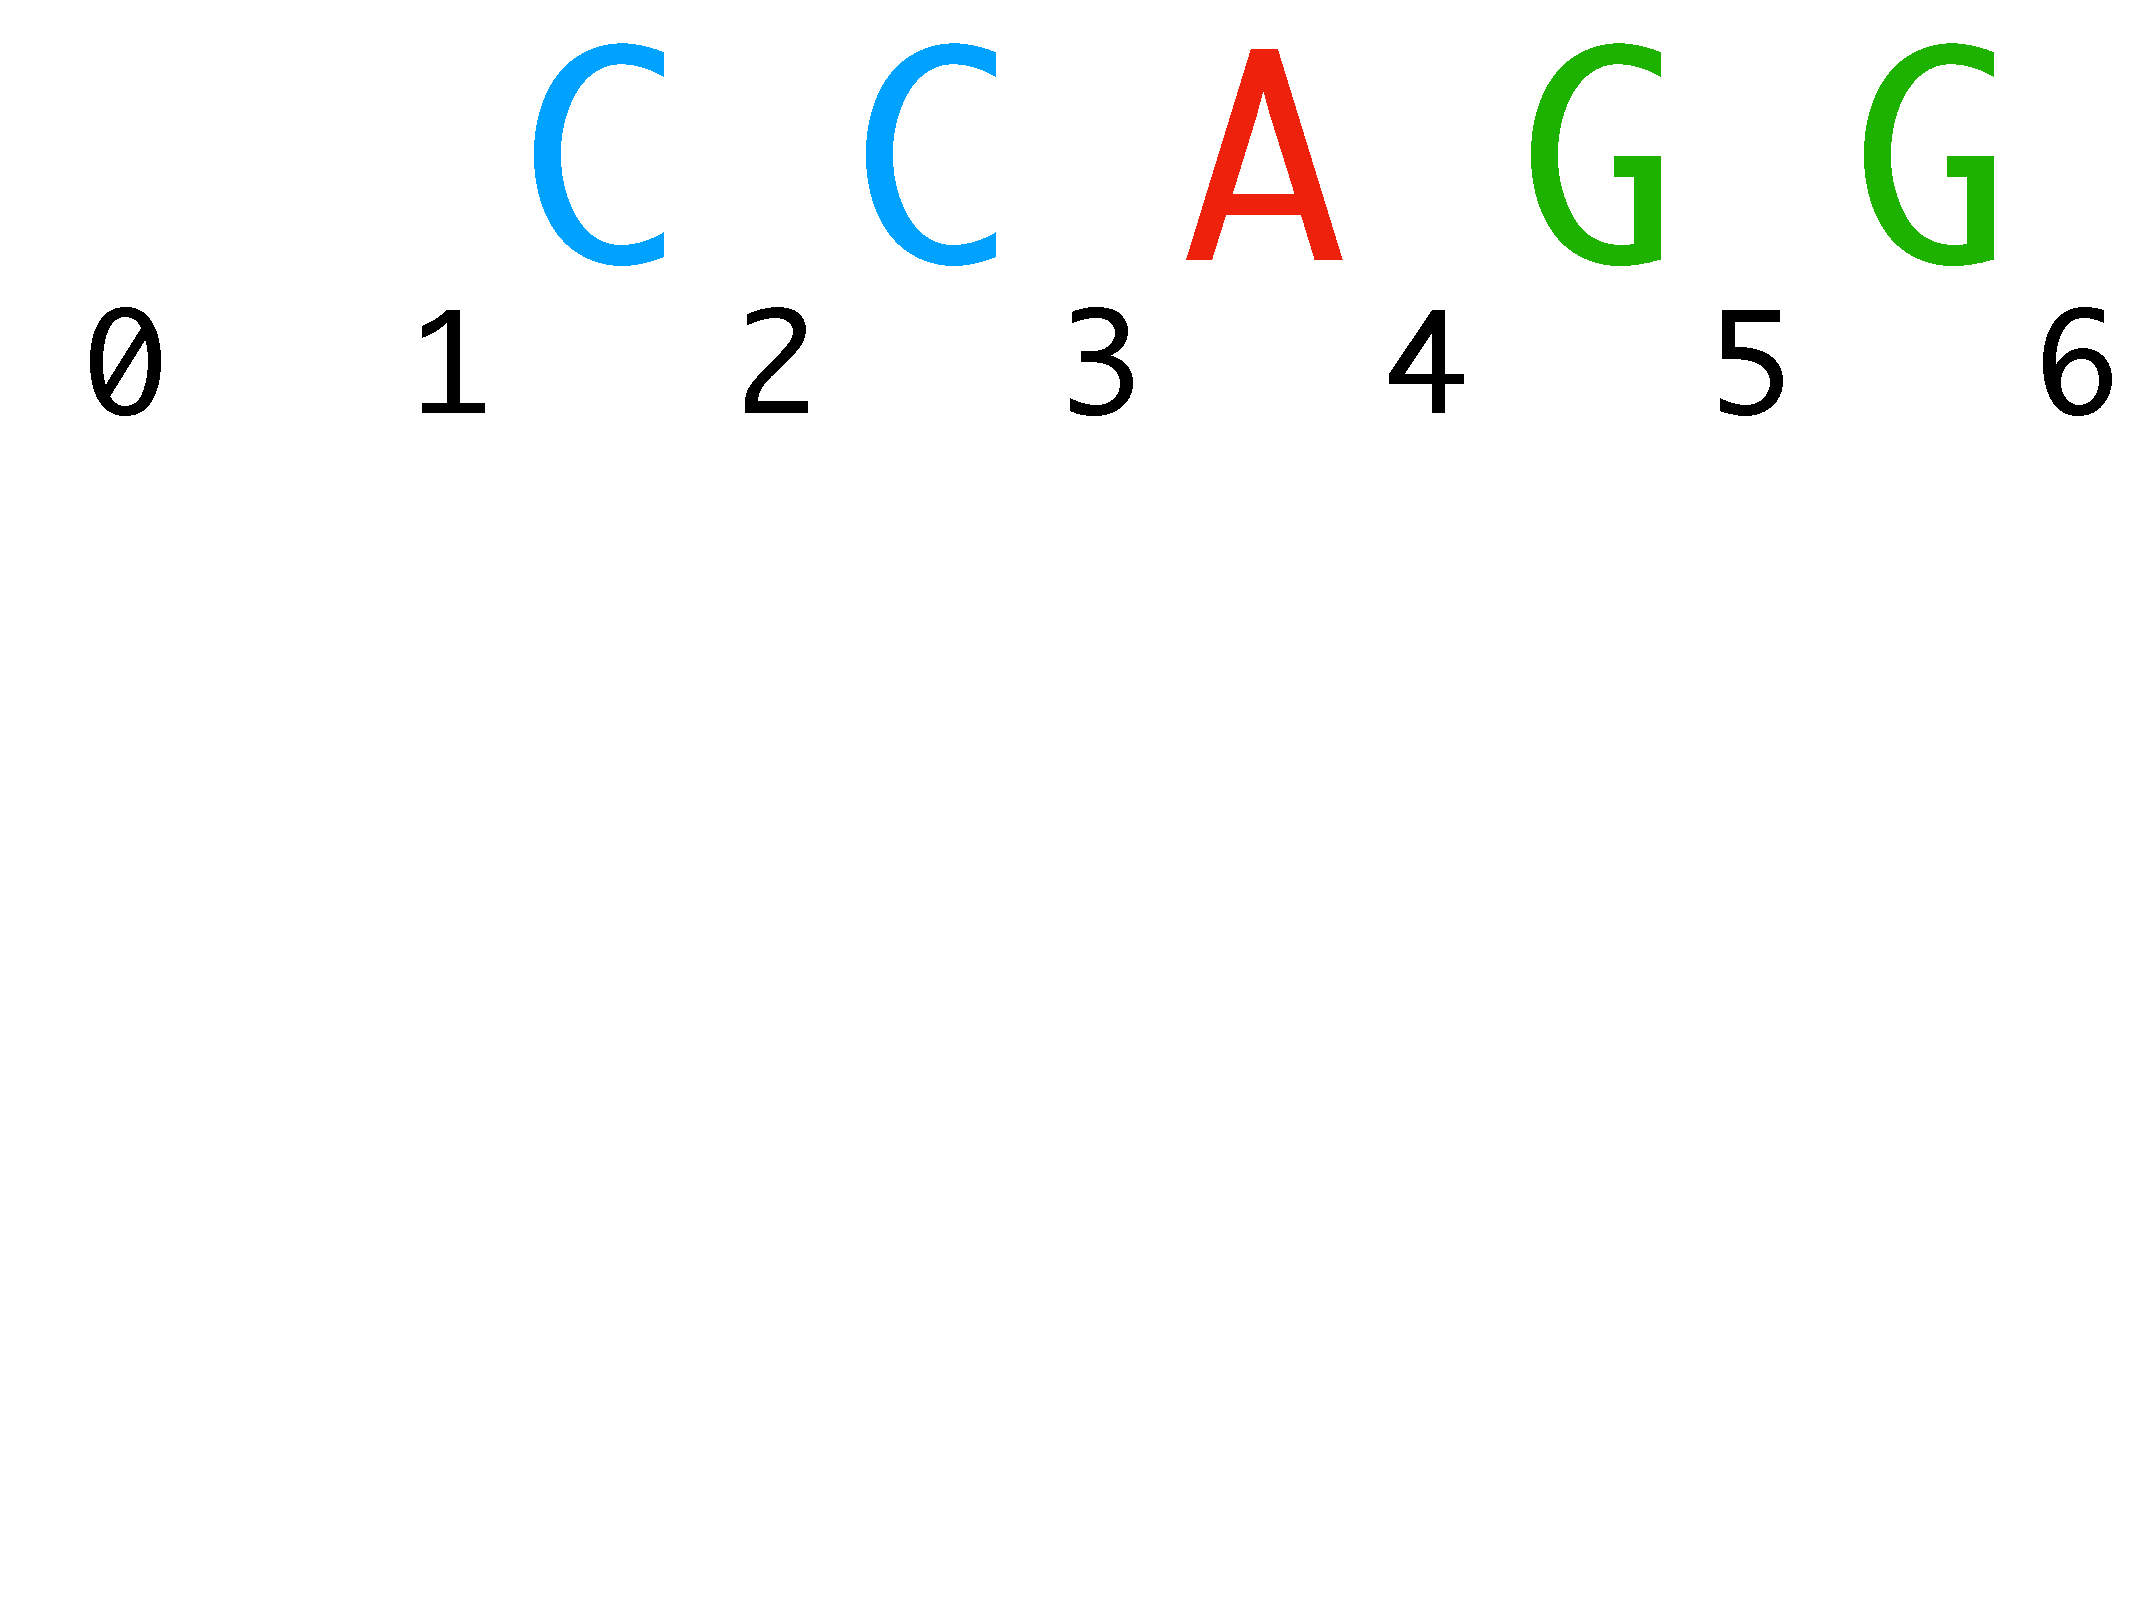
\includegraphics[scale=.16]{figs/index} \\[-3.cm]
%\hspace{-0.23cm}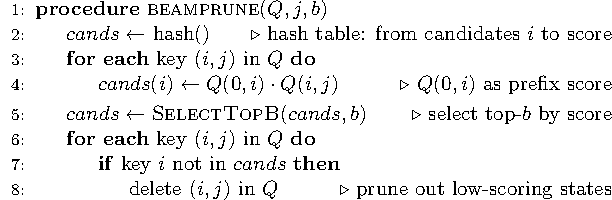
\includegraphics[scale=1.2]{figs/beam_prune_alg} \\[0.5cm]
  \algrenewcommand\algorithmicindent{1.5em}%
\begin{minipage}{0.85\textwidth}
\begin{algorithmic}[1]
  \newcommand{\INDSTATE}[1][1]{\State\hspace{#1\algorithmicindent}}
  \setstretch{1.2} % lhuang: usepackage setspace
\Function{beamprune}{$Q, j, b$}
    \State $\candidates \gets$ hash() \Comment{hash table: from candidates $i$ to score}
    \ForEach{$i$ such that $[i,j]$ in $Q$}
        \State $\candidates[i] \gets \Qf{1}{i-1} \cdot \Qf{i}{j}$ \Comment{like \linearfold, use $\Qf{1}{i-1} $ as prefix score}
    \EndFor
    \State $\candidates \gets \textsc {SelectTopB}(candidates, b)$ \Comment{select top-$b$ states by score}
    \ForEach{$i$ such that $[i,j]$ in $Q$}
        \If{key $i$ not in $candidates$}
            \State {\bf delete} $[i,j]$ from $Q$ \Comment{prune low-scoring states}
        \EndIf
    \EndFor
\EndFunction
\end{algorithmic}
% \end{algorithm}
\end{minipage}
\caption{
The {\sc BeamPrune} function from the Pseudocode of our main algorithm (Fig.~\ref{fig:algorithm}).
\label{fig:beam_prune_alg}}
% \vspace{-0.3cm}
% \end{figure*}
\end{figure}x


\begin{figure}[h]%[b]
  % \newcommand{\pluseq}{\mathrel{+}=}
\center
\small
\algrenewcommand\algorithmicindent{1.5em}%
  % \algnewcommand\algorithmicforeach{\textbf{for each}}
\algdef{S}[FOR]{ForEach}[1]{\algorithmicforeach\ #1\ \algorithmicdo}
% \hspace{-0.23cm}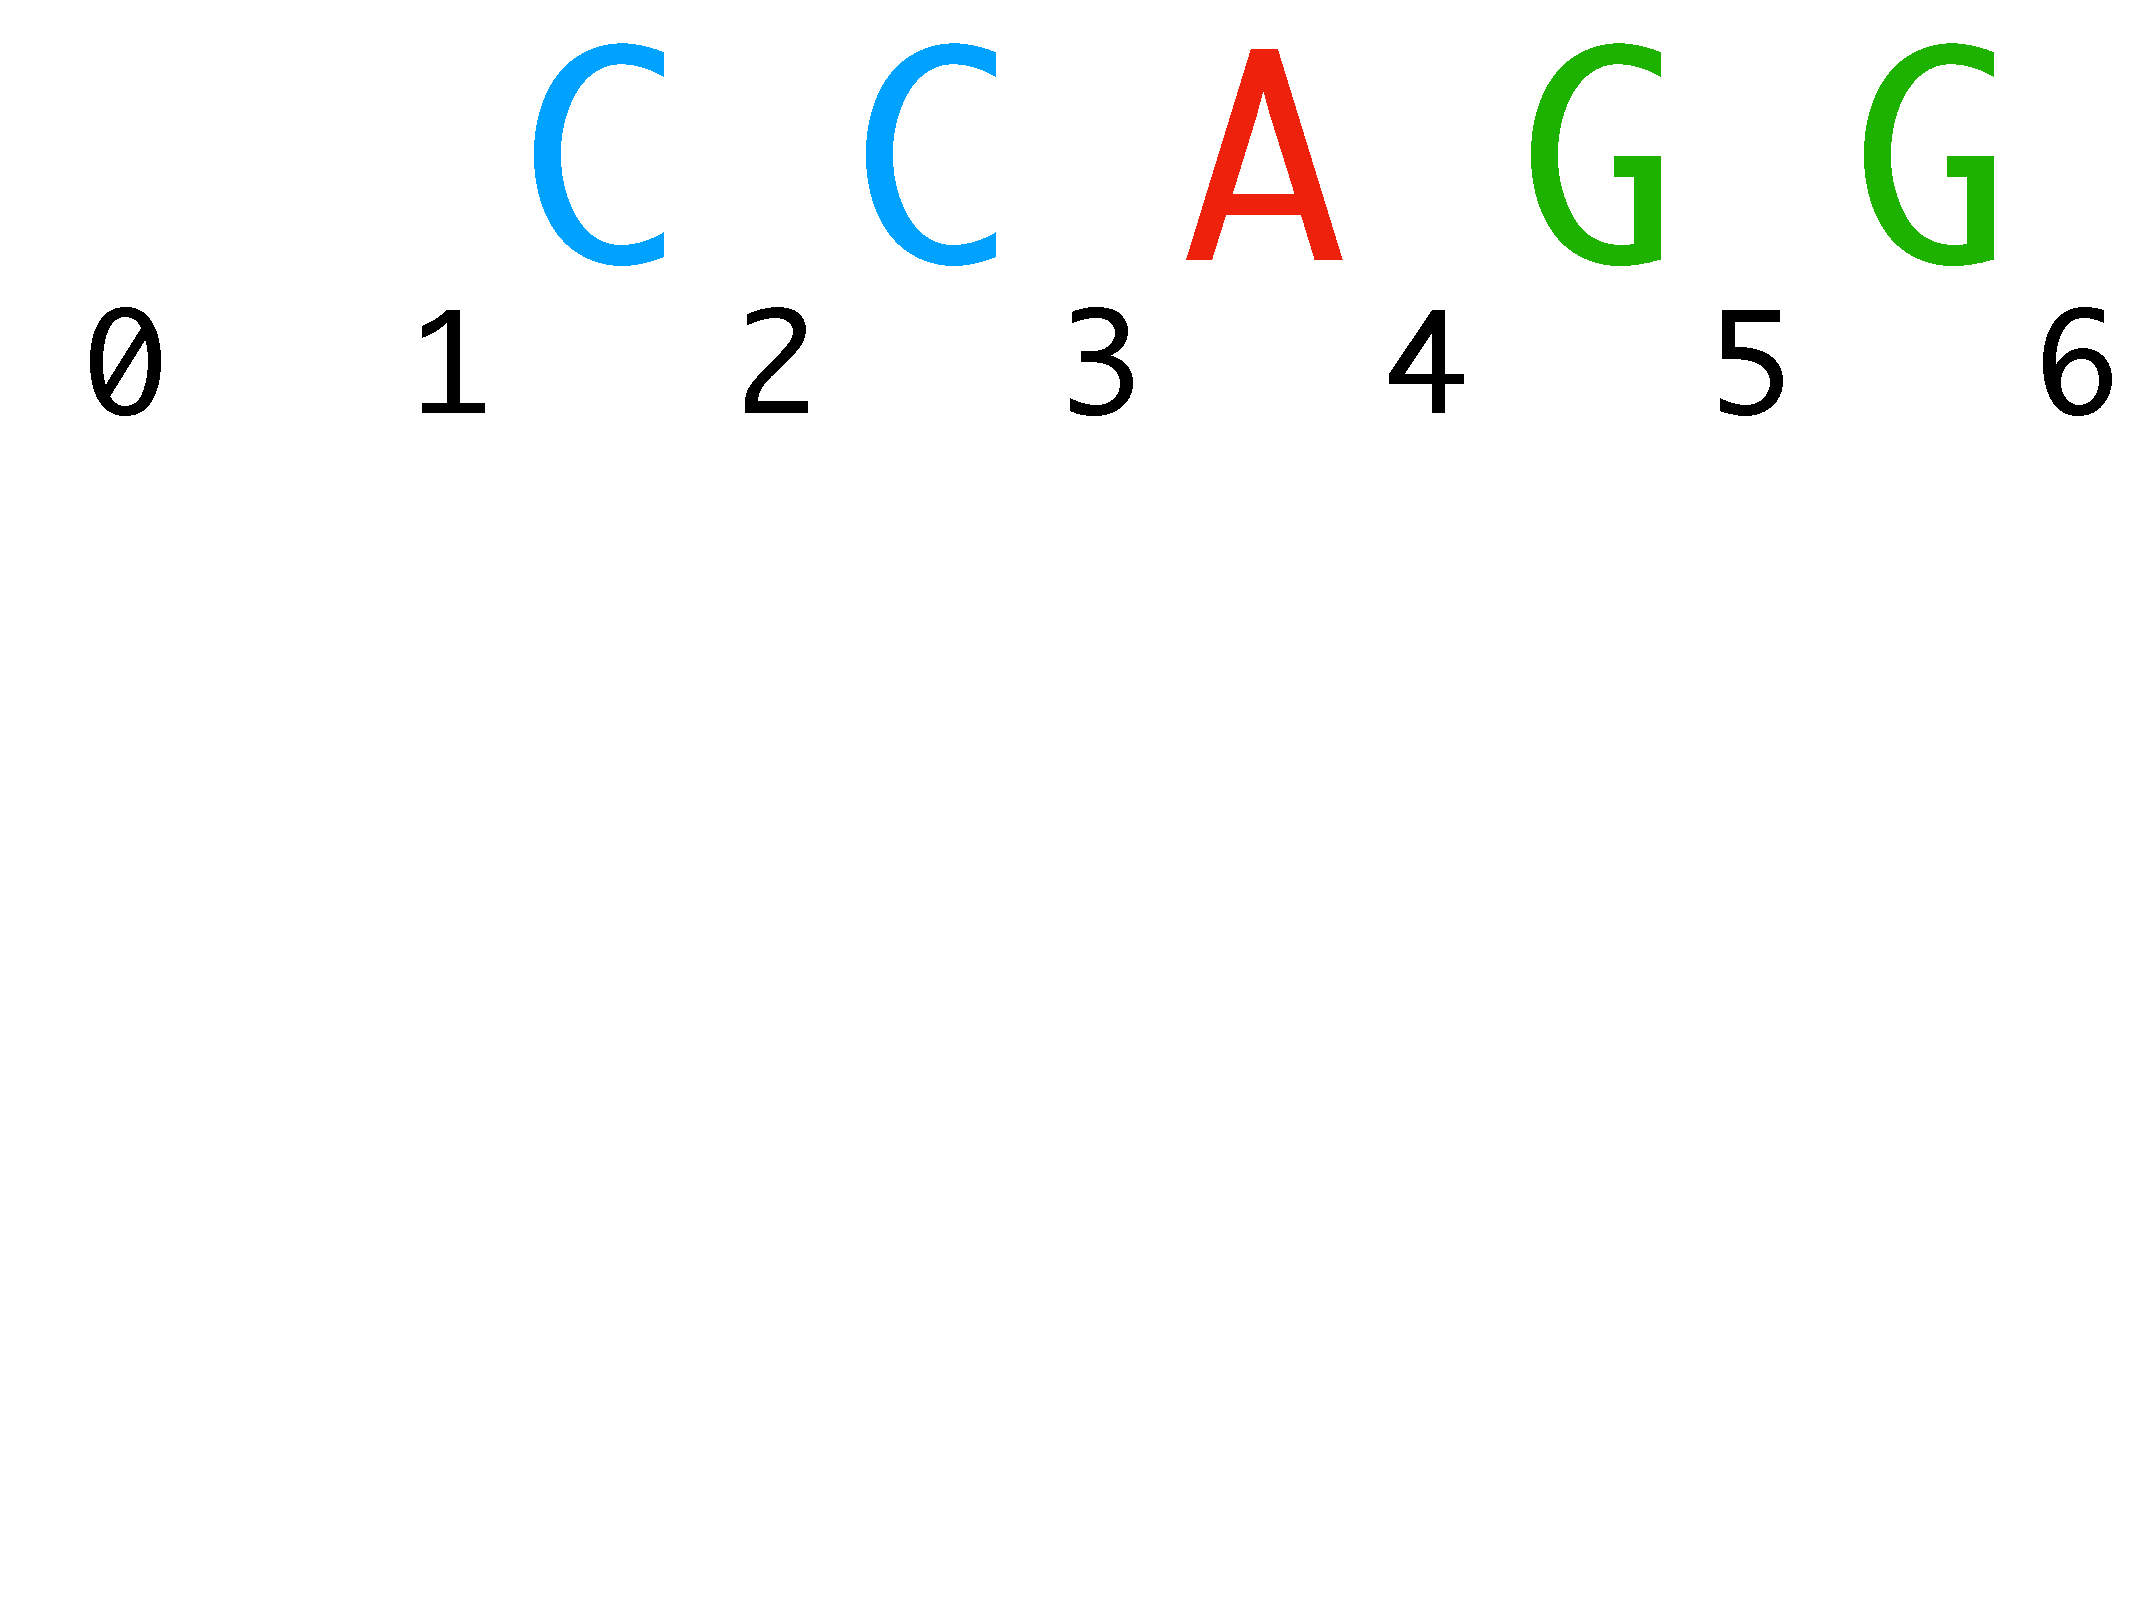
\includegraphics[scale=.16]{figs/index} \\[-3.cm]
%\hspace{-0.23cm}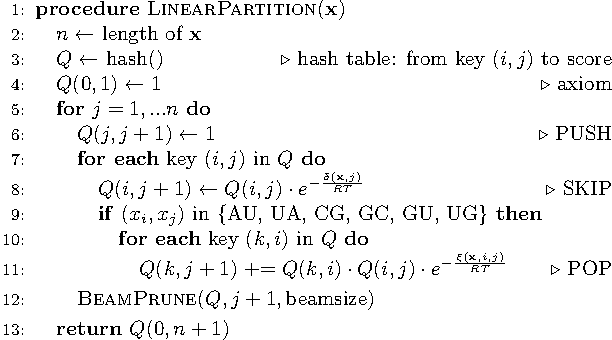
\includegraphics[scale=.83]{figs/algorithm} \\[0.2cm]
\begin{minipage}{.85\textwidth}
\begin{algorithmic}[1]
  \newcommand{\INDSTATE}[1][1]{\State\hspace{#1\algorithmicindent}}
  \setstretch{1.2} % lhuang: usepackage setspace
\Function{BasePairingProbs}{$\vecx, Q$}  \Comment{outside calculation}
% \bindent
    \State $n \gets$ length of $\mathbf x$
    \State $\Qhat \gets$ hash() \Comment{hash table: from span $[i,j]$ to $\Qhatf{i}{j}$: outside partition function}
    \State $p \gets$ hash() \Comment{hash table: from span $[i,j]$ to $p_{i,j}$: base-pairing probs}
    % \State $Q[j,\,j-1] \gets 1$ for all $j$ in $1...n$ \Comment{base cases} \label{line:base}
    \State $\Qhatf{1}{n} \gets 1$ \Comment{base case}
    \For{$j=n$ {\bf downto } $1$}
        \ForEach {$i$ such that $[i,\,j-1]$ in $Q$}\smallskip
            \State $\Qhatf{i}{j-1} \pluseq \Qhatf{i}{j} \cdot e^{-\frac{\delta(\vecx,j)}{RT}} $ \Comment{\nskip} \label{line:skip}
            \If{$x_{i-1}x_j$ in \{AU, UA, CG, GC, GU, UG\}}  \label{line:pair}
                % \State $Q_{i,\,j+1} \gets  C(i,\,j) \cdot e^{-\frac{\xi(\vecx,i,\,j)}{RT}} $
                \ForEach{$k$ such that $[k,\,i-2]$ in $Q$}\smallskip
                    \State $\Qhatf{k}{i-2} \pluseq {\Qhatf{k}{j} \cdot \Qf{i}{j-1} \cdot e^{-\frac{\xi(\vecx,i-1,j)}{RT}}}$ \Comment{\pop: left} %\label{line:pop}
                    % \State $C(0,j+1) \pluseq {C(0,k) \cdot C(k,j+1) \cdot e^{-\frac{\xi(\vecx,i,\,j)}{RT}}} $
                    \State $\Qhatf{i}{j-1} \pluseq {\Qhatf{k}{j} \cdot \Qf{k}{i-2} \cdot e^{-\frac{\xi(\vecx,i-1,j)}{RT}}}$ \Comment{\pop: right} %\label{line:pop}
                    \State $p_{i-1,\,j} \pluseq \displaystyle\frac{\Qhatf{k}{j} \cdot \Qf{k}{i-2}  \cdot  e^{-\frac{\xi(\vecx,i-1,j)}{RT}} \cdot \Qf{i}{j-1}}{\Qf{1}{n}}$ \Comment{accumulate base pairing probs}
                \EndFor
                % \State $C(0,j+1) \pluseq C(0,i) \cdot Q_{i,j+1}$ \Comment{COMBINE}
            \EndIf
        \EndFor
        %% \ForEach {$i$ such that $[i,\,j]$ in $P$}\smallskip
        %%          \State $p_{i,j} = \frac{\hatp[i,\,j] \cdot Q[i+1,\, j-1]}{Q[1,n]}$
        %% \EndFor
        % \State $\textsc {BeamPrune}(Q,j+1, b)$ \Comment{see Fig.~\ref{fig:beam_prune_alg}}
    \EndFor
    \State \Return $p$ \Comment{return the (sparse) base-pairing probability matrix}
% \eindent
\EndFunction
%% \Function{BasePairingProbabilities}{$\vecx, Q, \hatp$} % \Comment{$Q$ is the beam size}
%% % \bindent
%%     \State $p \gets$ hash() \Comment{hash table: from span $[i,j]$ to base pairing probability $p_{i,j}$}
%%     \For{$j=2 ... |\vecx|$}
%%       \ForEach {$i$ such that $[i,j]$ in $\hatp$}
%%           \State $p_{i,j} = \displaystyle\frac{\hatp[i,\,j] \cdot Q[i+ 1,\, j-1] \cdot  e^{-\frac{\xi(\vecx,i,j)}{RT}}}{Q[1,n]}$
%%       \EndFor
%%     \EndFor
%%     \State \Return the (sparse) base-pairing probability matrix $p$
%% \EndFunction
\end{algorithmic}
\end{minipage}
\caption{
  Outside partition function and base pairing probabilities calculation for a simplified version of the \linearpartition.
  $Q$ is the (inside) partition function calculated by the pseudocode in Fig.~\ref{fig:algorithm}, and $\Qhat$ is the outside partition function. 
% as well as a beam prune algorithm. 
% Here we model hash tables following Python dictionaries, where $(i, j) \in C$ checks whether the key $(i, j)$ is in the hash $C$; 
% this is needed to ensure linear runtime. 
% Quick select algotithm is used in beam prune, 
% and we skip the details for quick select here since it is well known.
% Real \linearpartition system is much more involved, but the pseudocode illustrates the left-to-right partition function calculation idea using a Nussinov-like fashion.
The actual algorithm using the Turner model is in our \href{https://github.com/LinearFold/LinearPartition}{GitHub codebase}.
%See Fig.~\ref{fig:beam_prune_alg} for {\sc BEAMPRUNE} function.
\label{fig:outside}}
\vspace{-0.3cm}
% \end{figure*}
\end{figure}


\iftrue
\begin{figure}[h]
  \centering
  \captionsetup{singlelinecheck=off}
%\hspace{-0.5cm}
\begin{tabular}{ll}
\hspace{-.5cm}{\panel A} & {\panel B}\\[-1cm]
    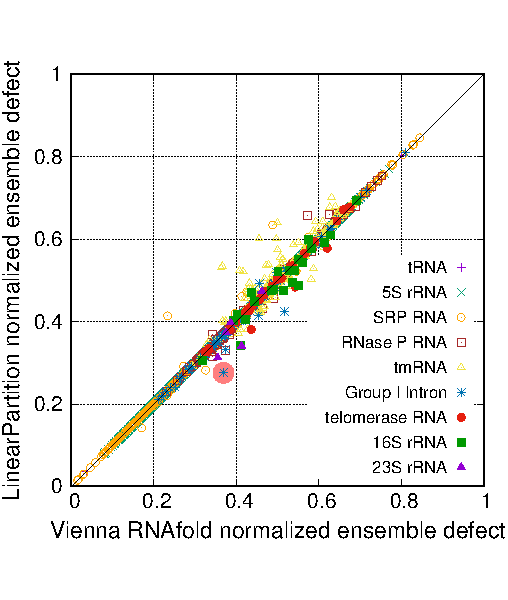
\includegraphics[width=.3\textwidth]{figs/norm_ensemble_defect}
    &
    \hspace{-0.1cm}
    \raisebox{.5cm}{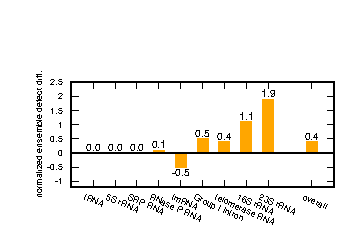
\includegraphics[width=.5\textwidth]{figs/onebar_norm_ensemble_defect_histogram}}
  \end{tabular} \\[-.3cm]
  \caption[.]{
  The 
  comparison of normalized ensemble defects (normalized by sequence length)
  % between \viennarnafold and \linearpartitionv 
  on the ArchiveII dataset.
  % Ensemble defects are normalized by sequence length. 
  {\bf A}: 
  Normalized ensemble defect between \viennarnafold and \linearpartitionv for each sequence; the trend is similar as Fig.~\ref{fig:ensemble}A, but the deviations for tmRNAs are more apparent; 
  the point with red shaded are the example in Fig.~\ref{fig:example}.
  {\bf B}: Normalized ensemble defect difference for each family; for longer families, 
  e.g., Group I Intron, telomerase RNA, 16S and 23S rRNA, 
  \linearpartition has lower normalized ensemble defect differences;
  note that \linearpartition's normalized ensemble defects are significantly better than \viennarnafold on Group I Intron ($p < 0.01$), 
  but significantly worse on tmRNA ($p < 0.01$).
  \label{fig:ensemble_defect}}
%\vspace{1cm}
\end{figure}
\fi

\iffalse
\begin{figure}[h]
  \centering
  \captionsetup{singlelinecheck=off}
\begin{tabular}{cccc}
\hspace{-4.4cm} \panel{A} & \hspace{-4.6cm}\panel{B} & \hspace{-4.6cm}\panel{C} & \hspace{-4.6cm}\panel{D}\\[-0.2cm]
\hspace{-0.2cm}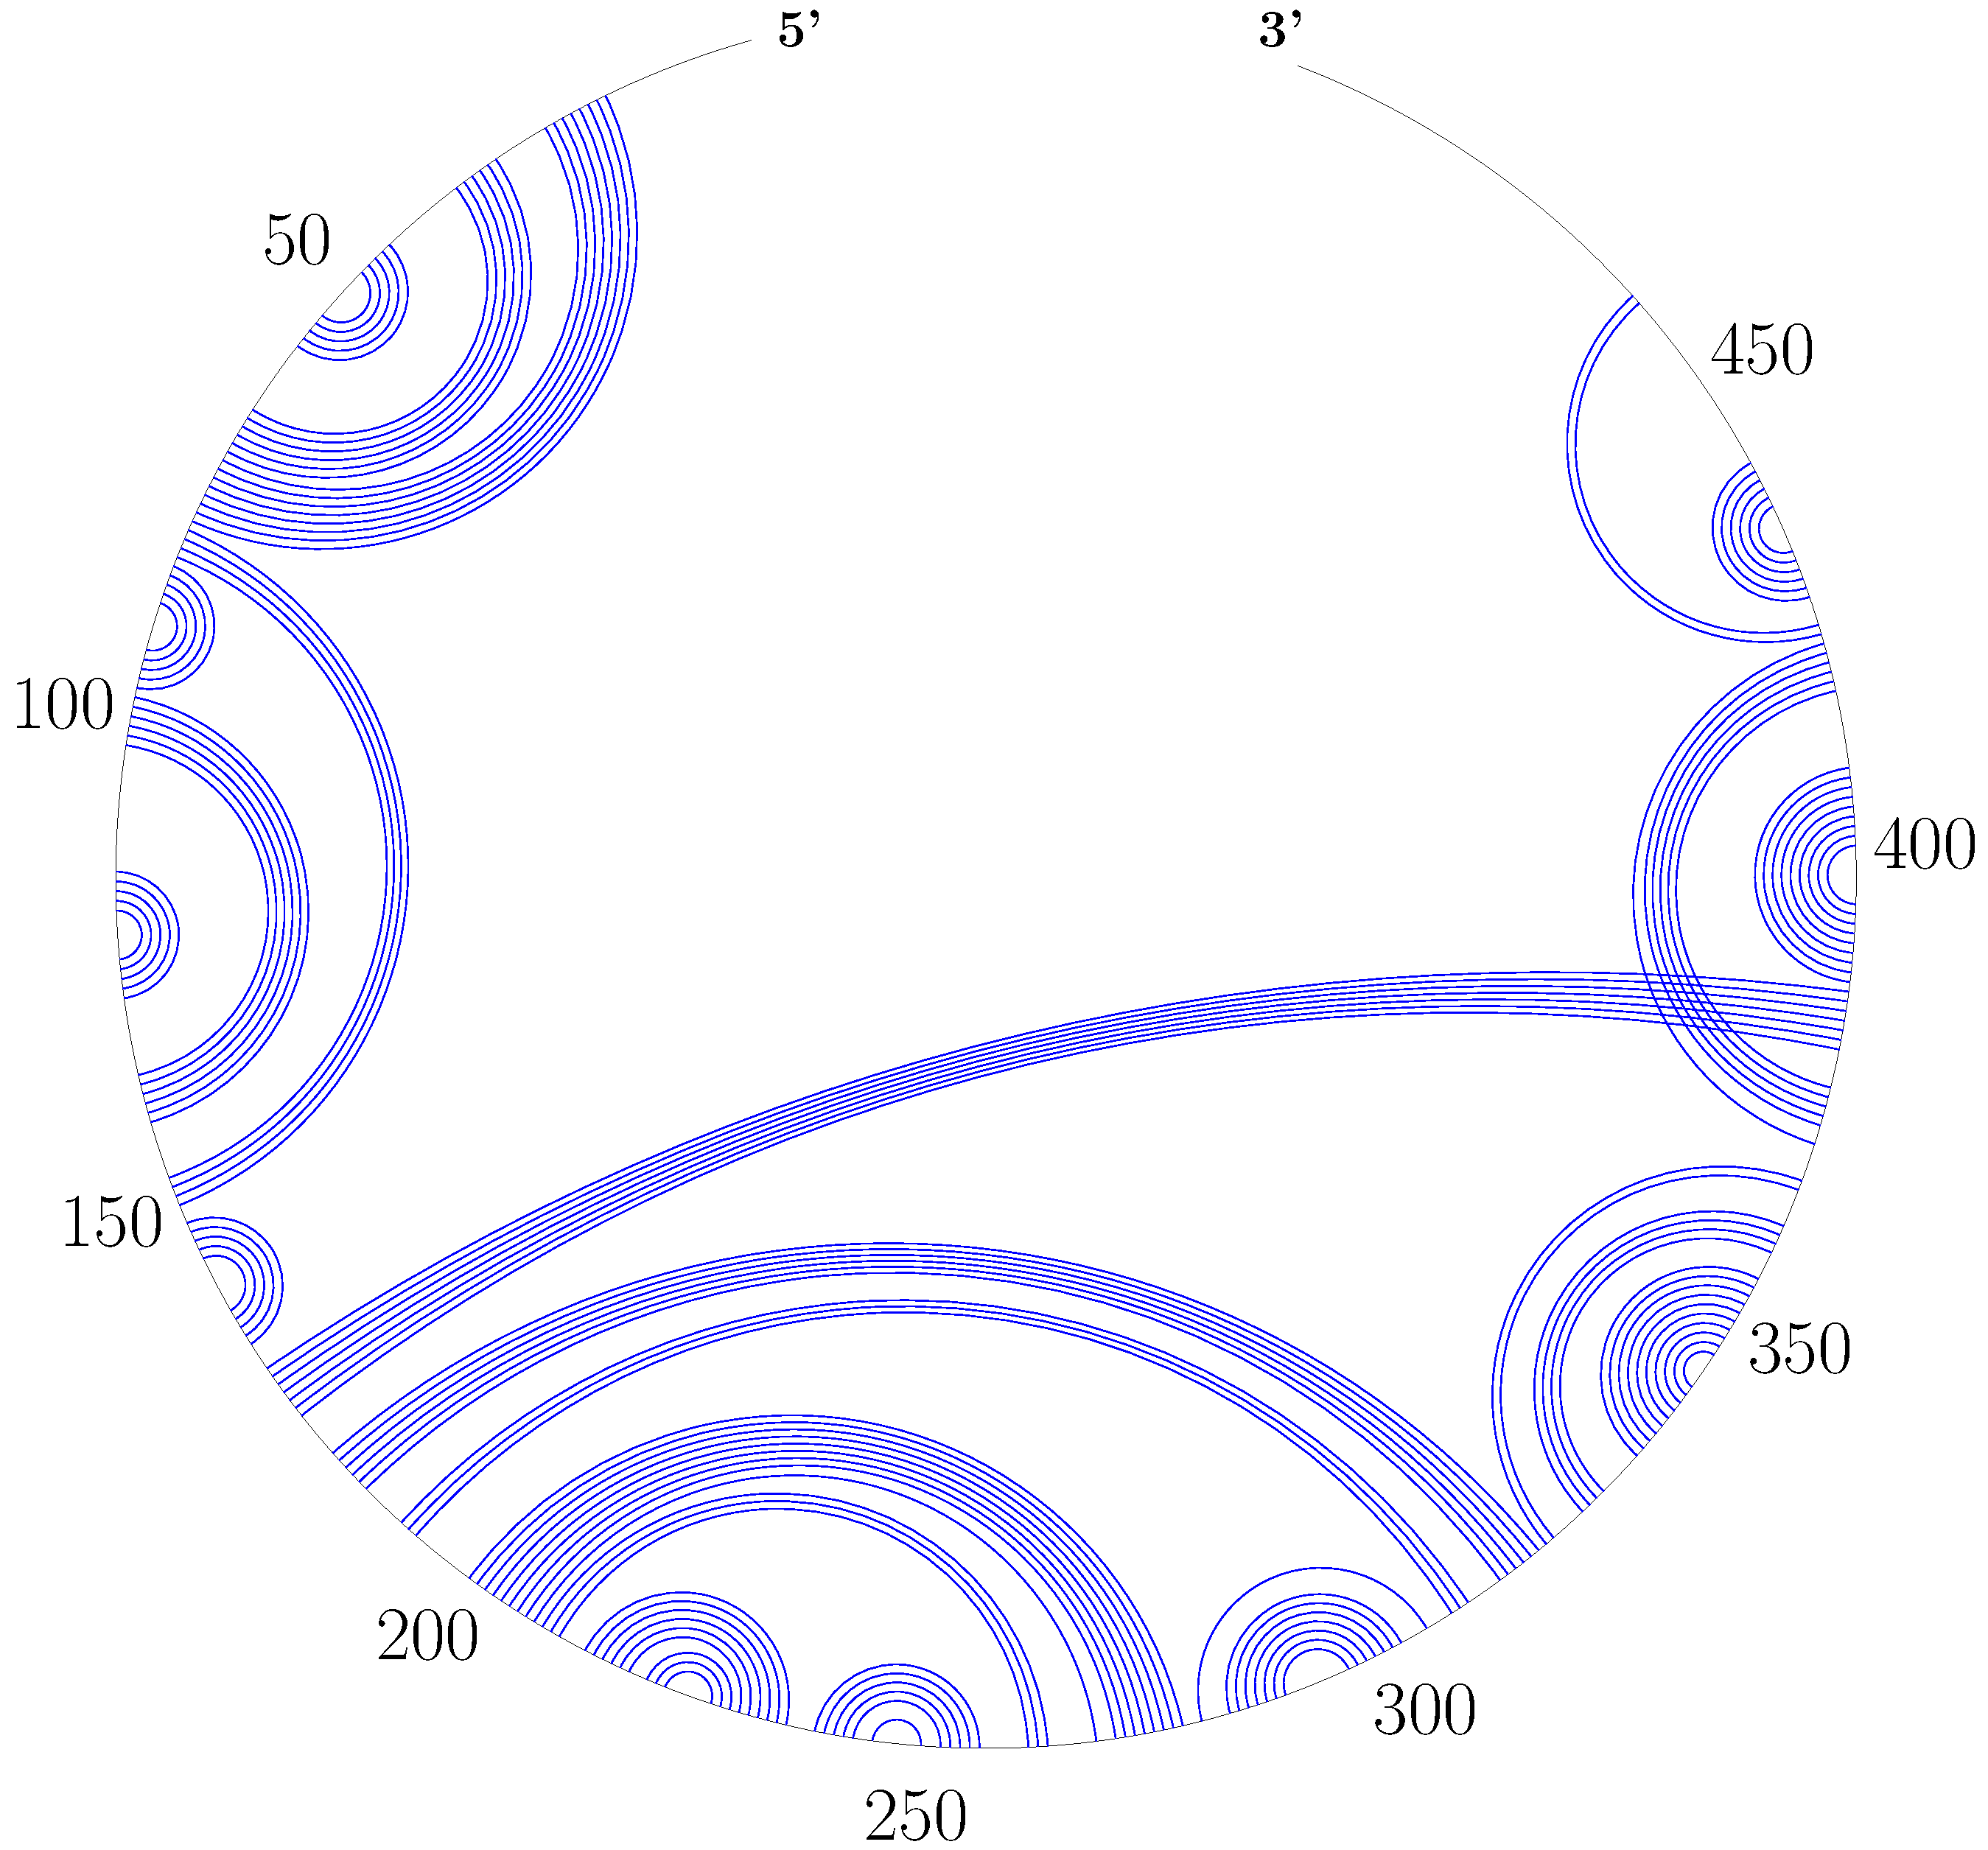
\includegraphics[width=0.25\textwidth]{figs/grp1_gold} &
\hspace{-0.35cm}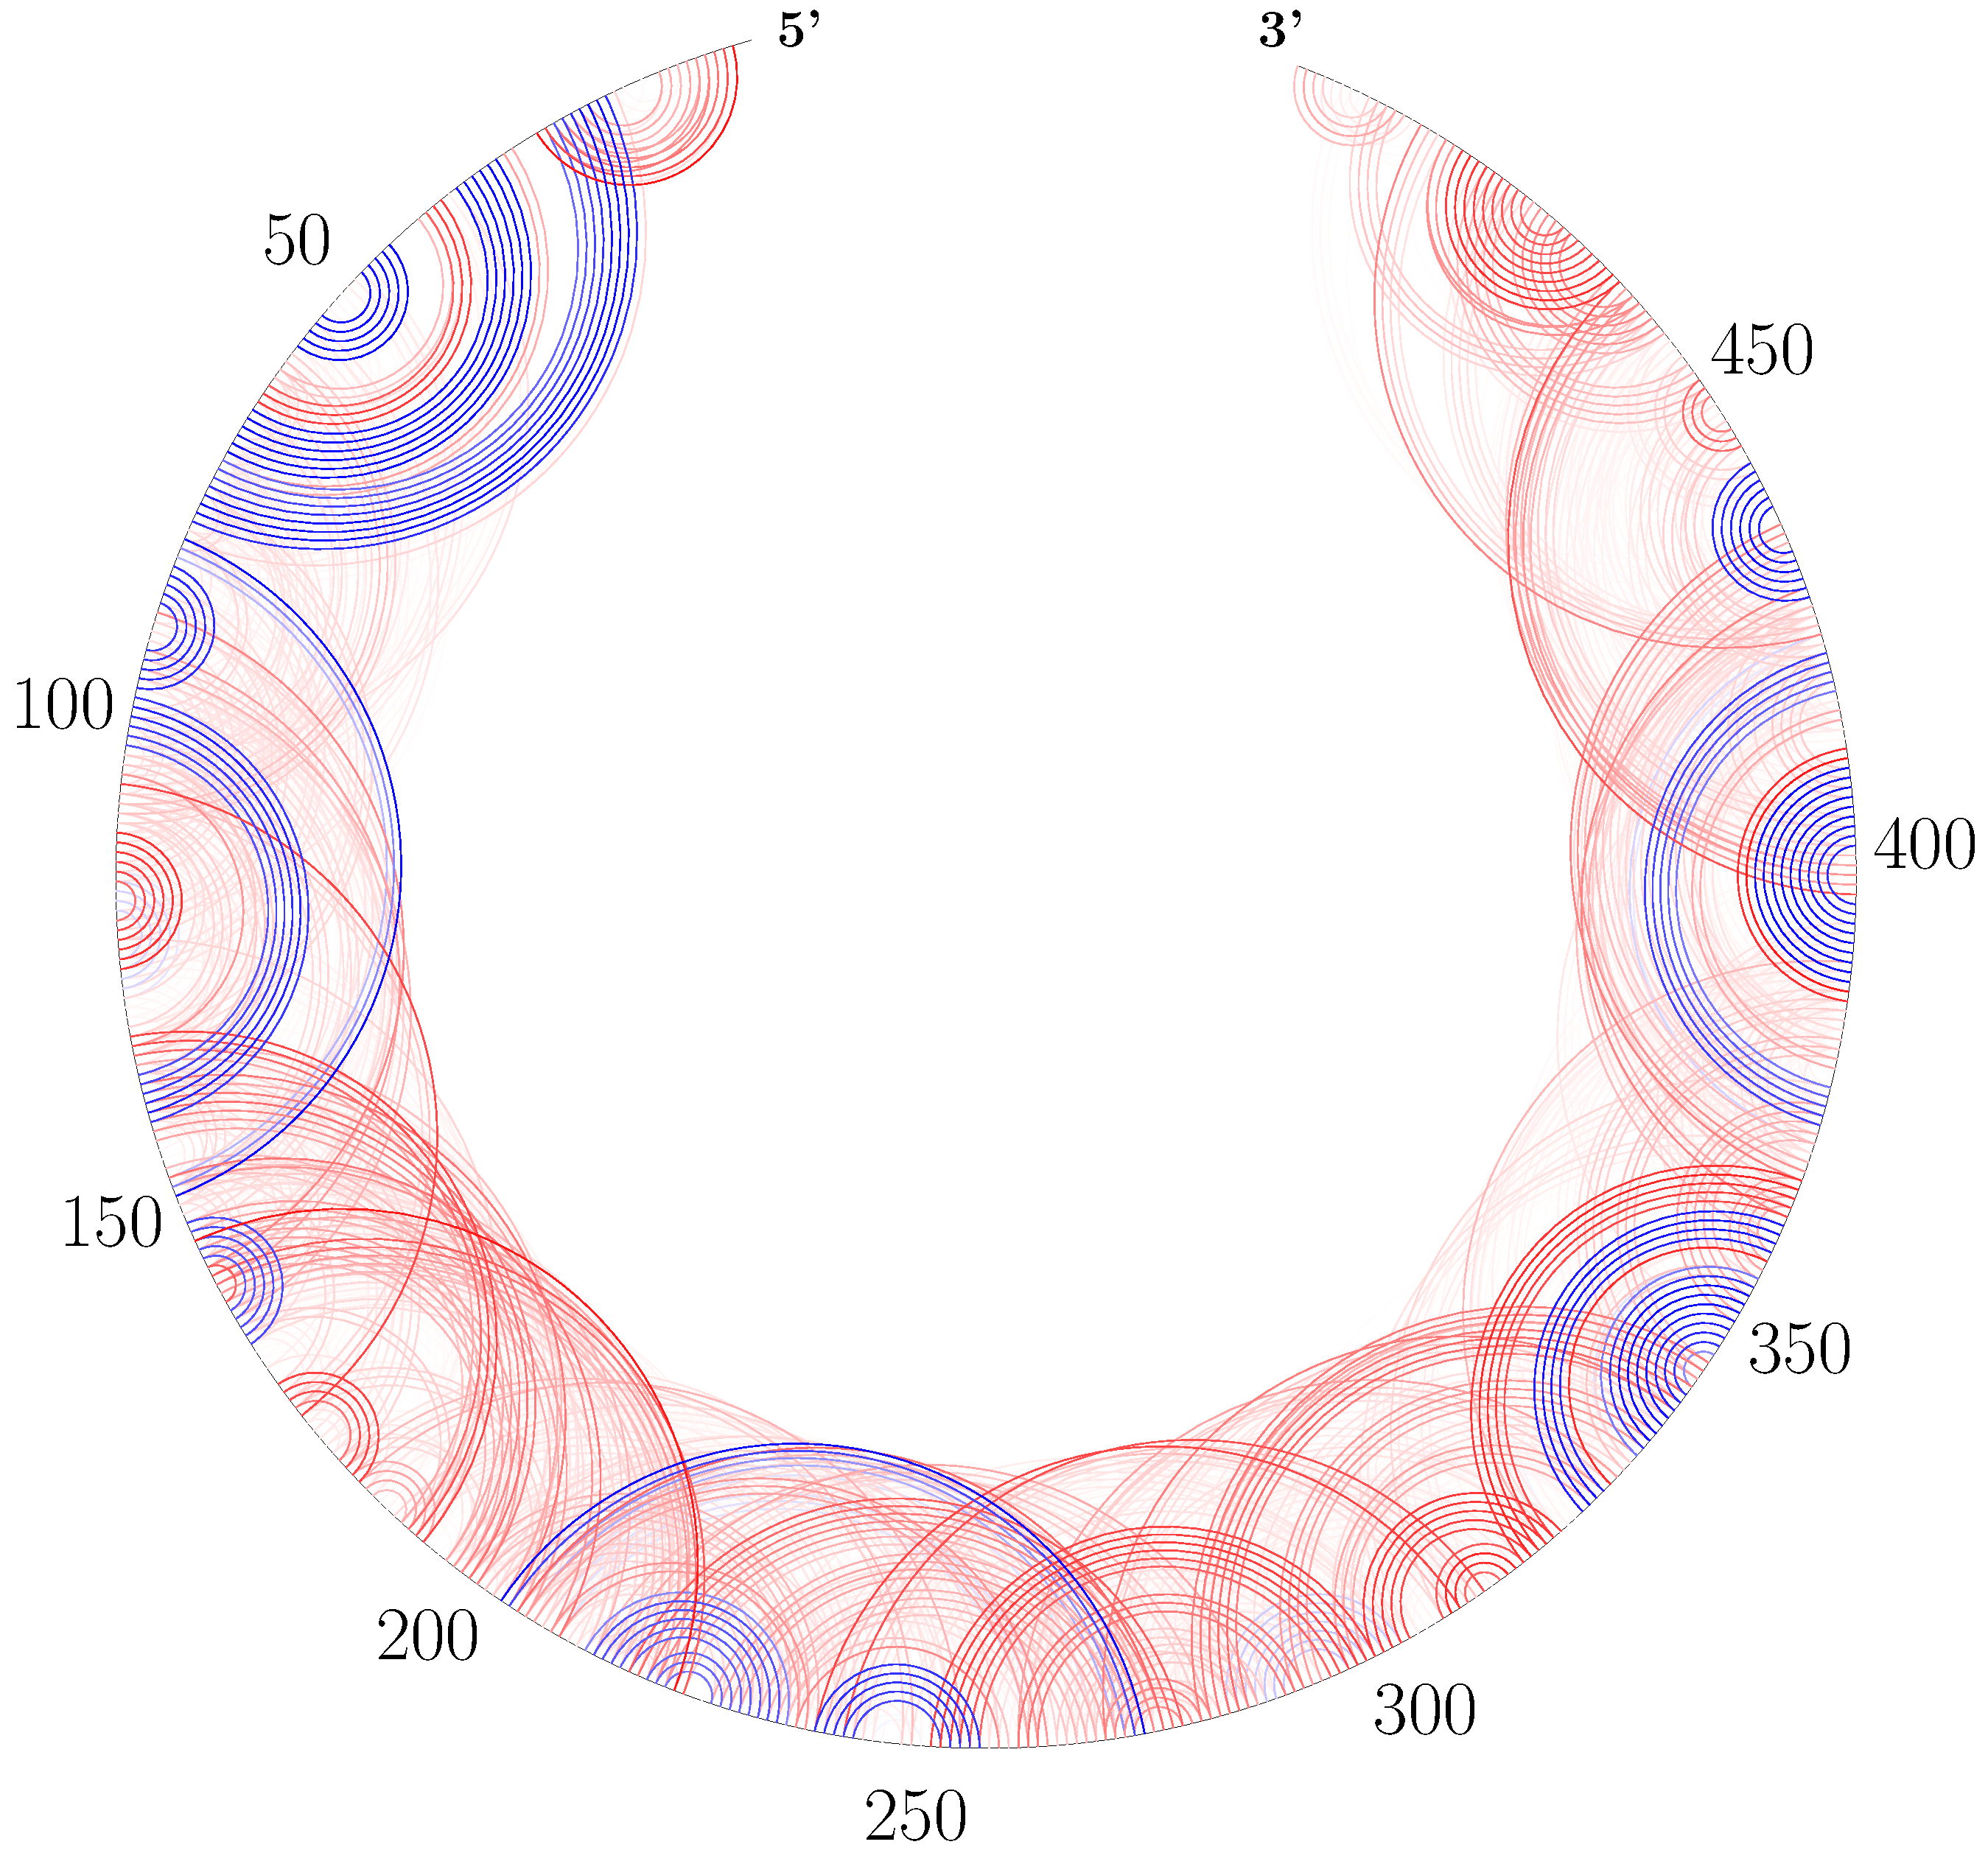
\includegraphics[width=0.25\textwidth]{figs/grp1_vienna_plfold_example.pdf} &
\hspace{-0.35cm}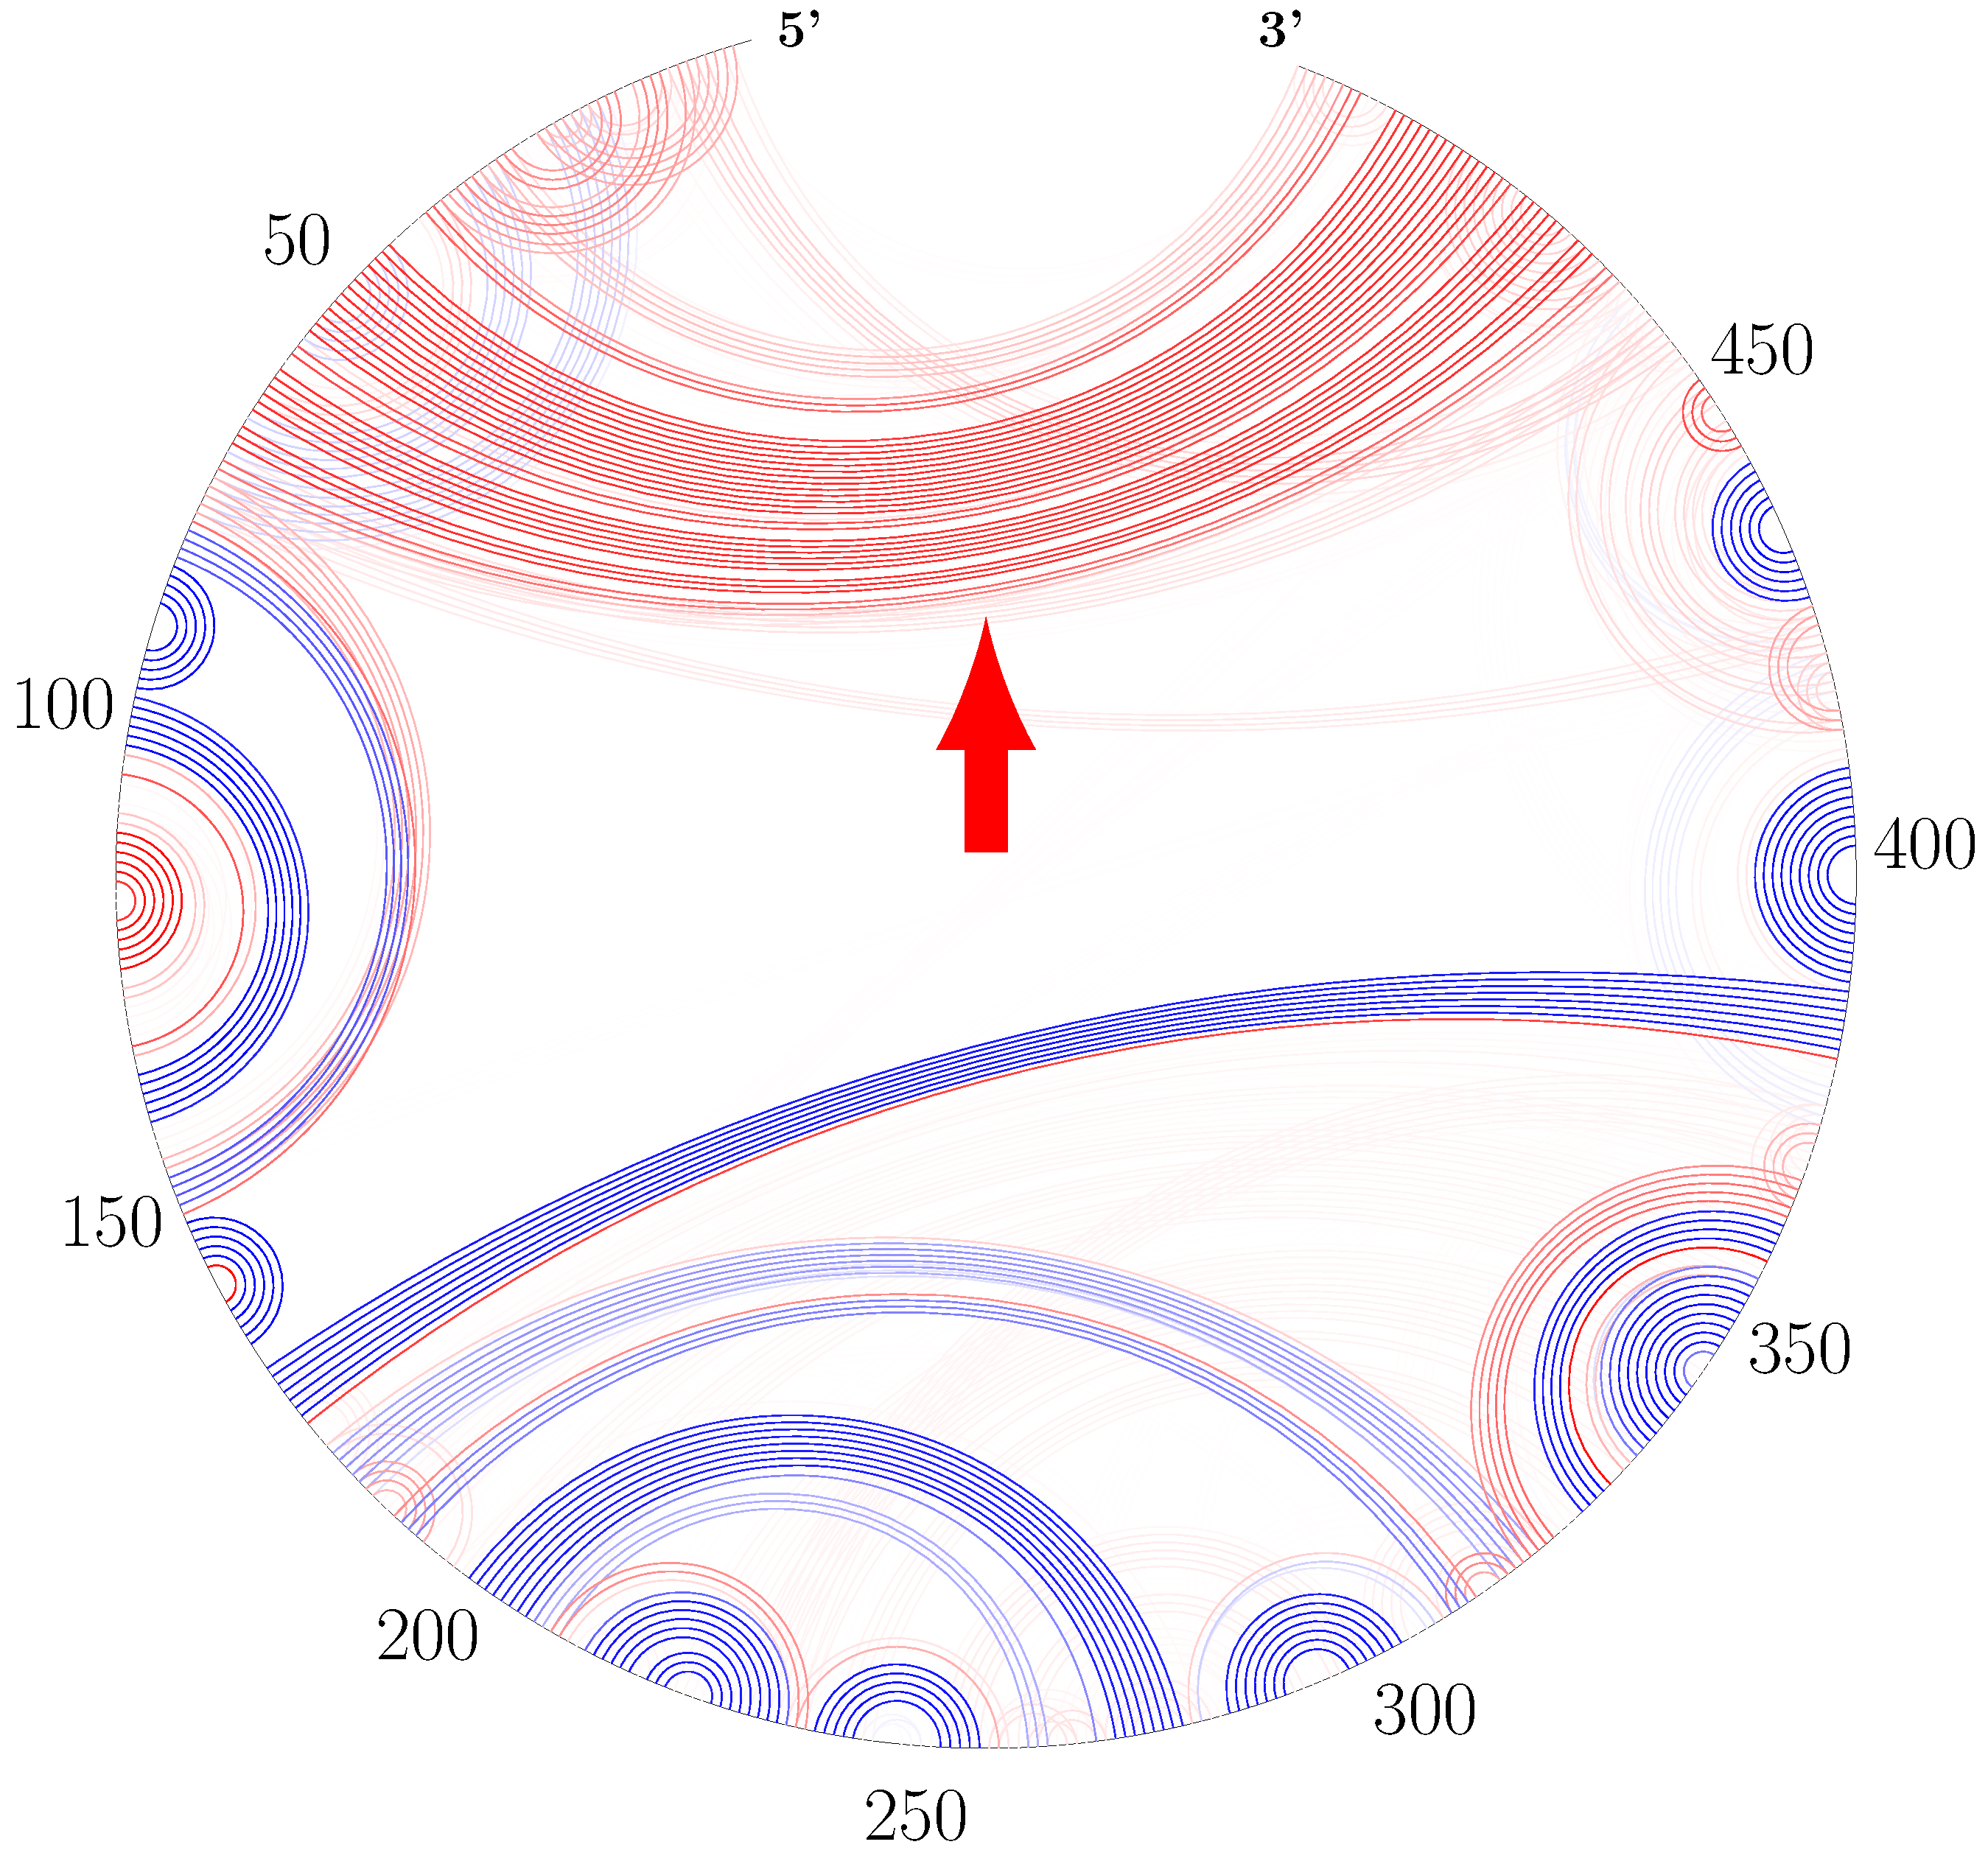
\includegraphics[width=0.25\textwidth]{figs/grp1_vienna_example} &
\hspace{-0.35cm}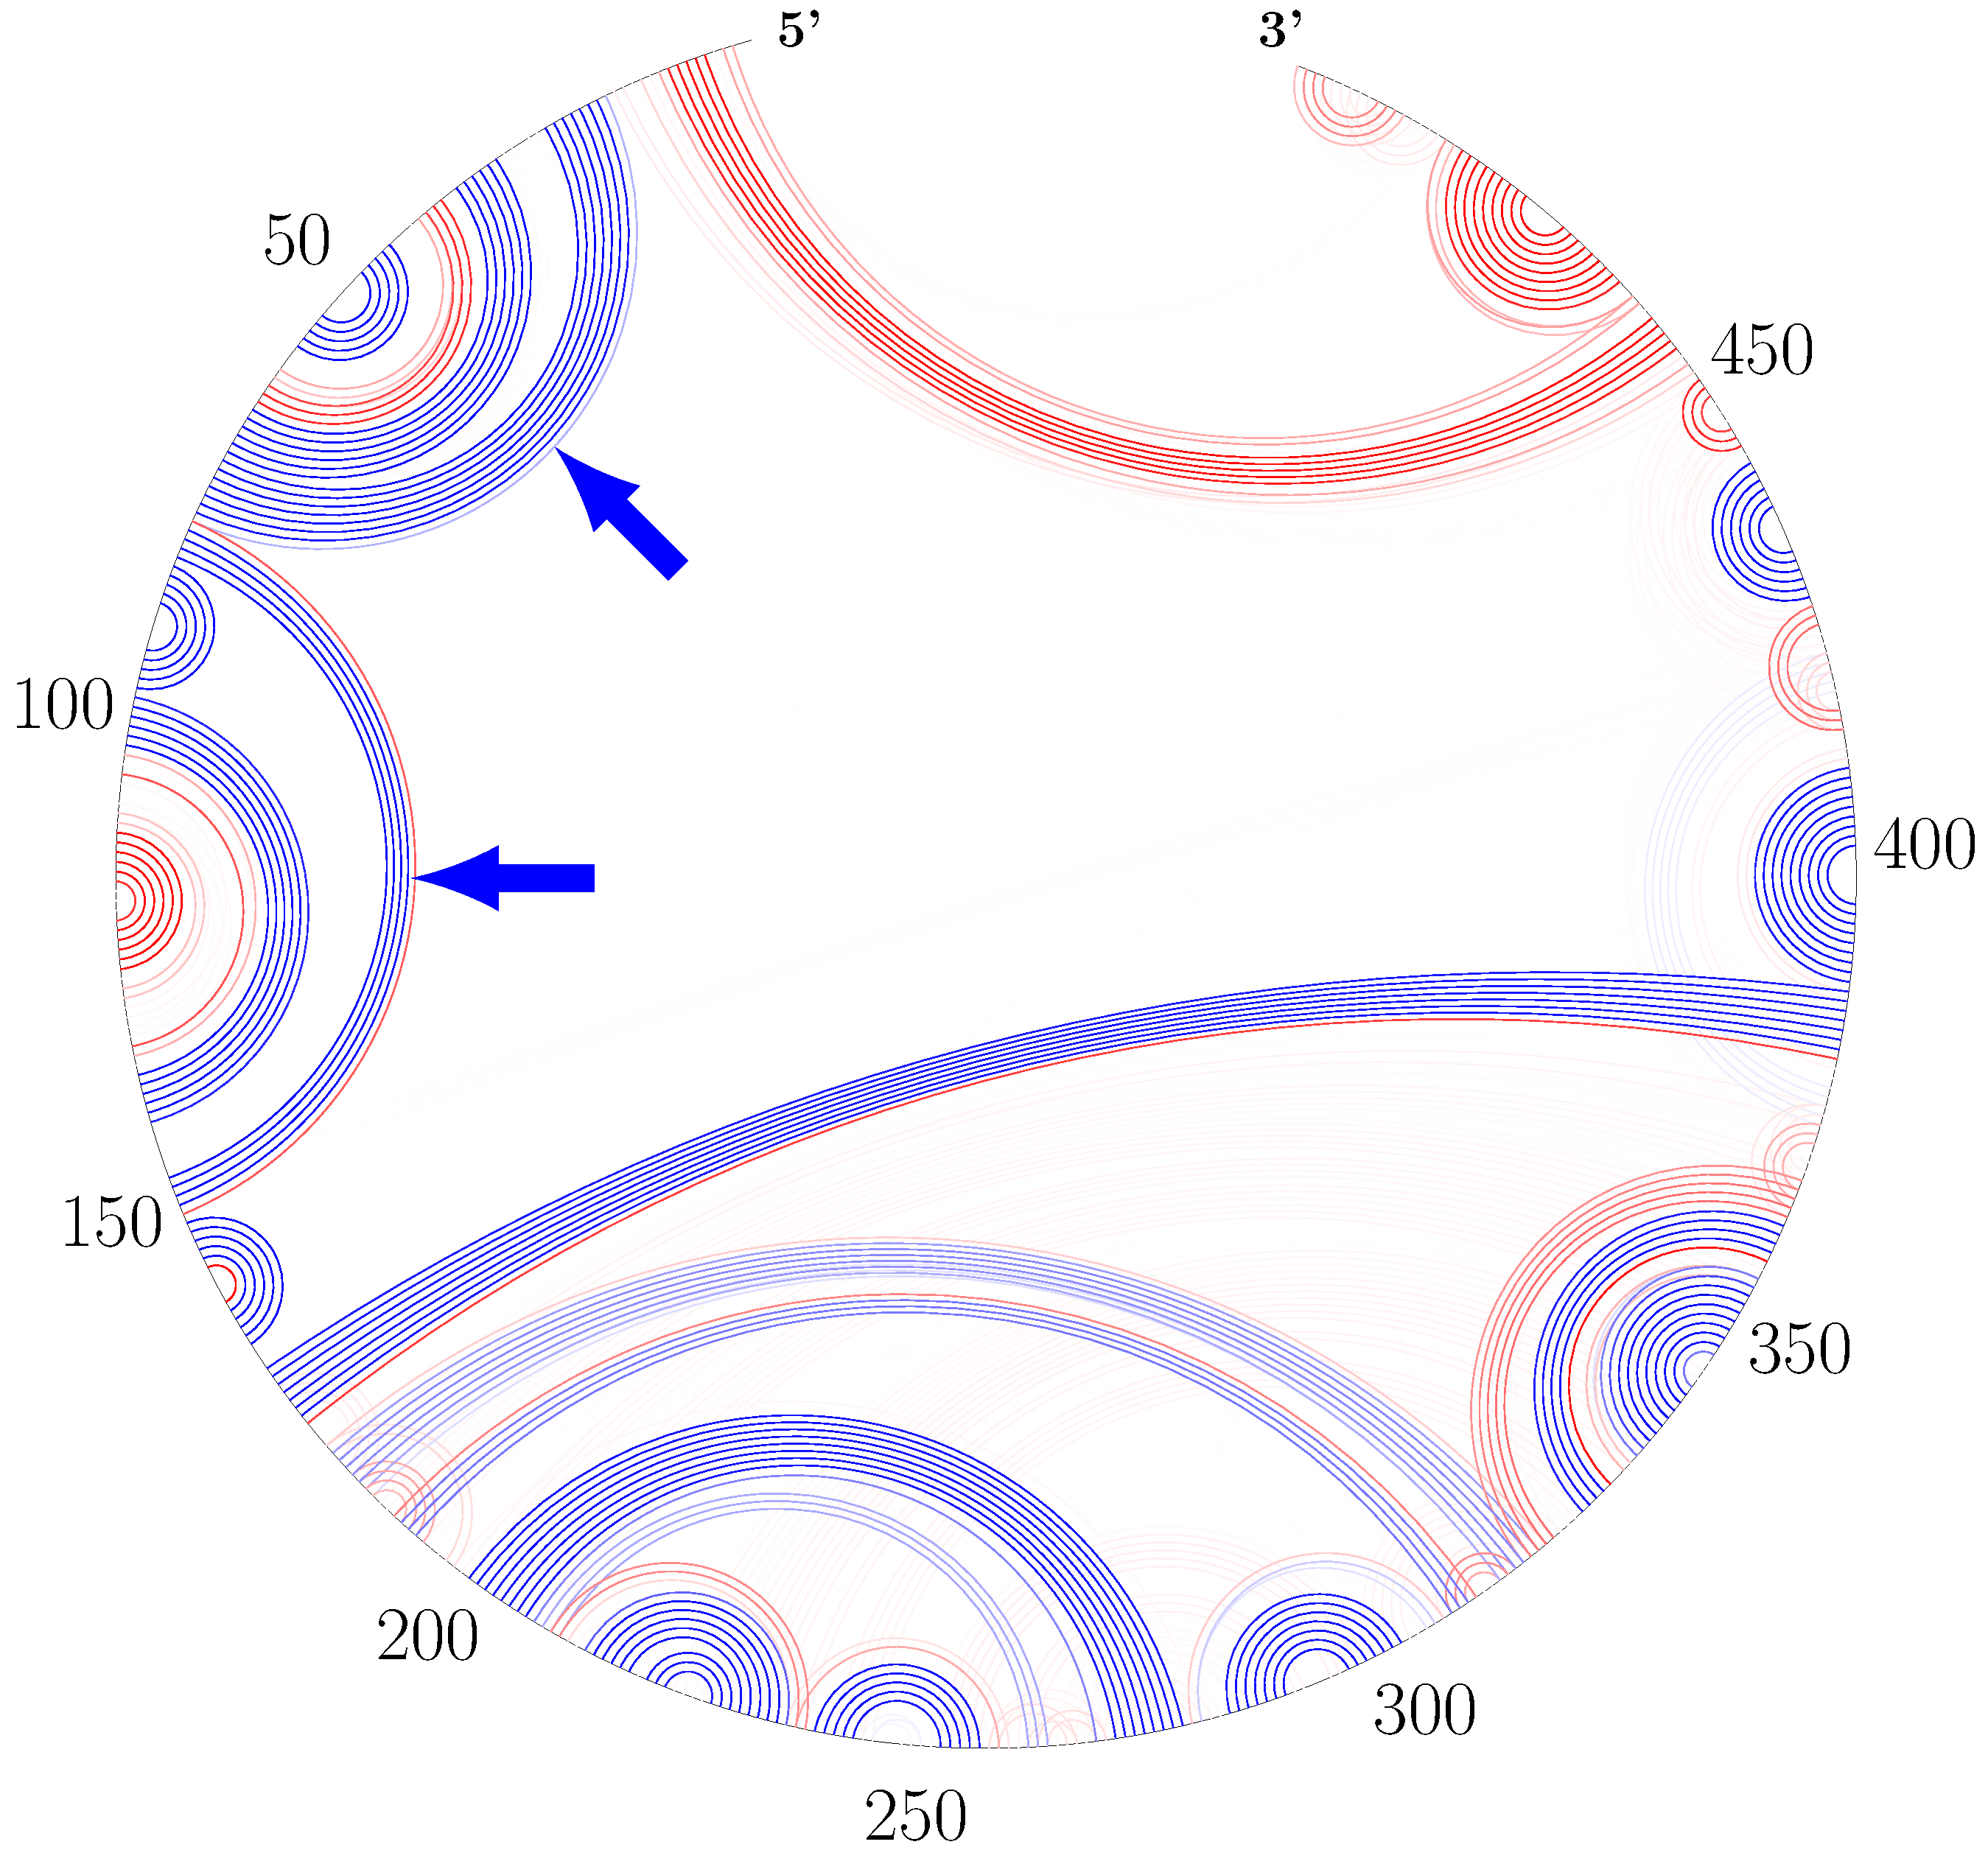
\includegraphics[width=0.25\textwidth]{figs/grp1_lpv_example.pdf}
\end{tabular}
  \caption[.]{Circular plots of {\it C.~ellipsoidea} Group I Intron.  
  Blue denotes pairs in the known structure and Red denotes predicted pairs not in the known structure.  
  The darkness of the line indicates pairing probability, 
  which the darkest lines close to a portability of 1. 
  {\bf A}: 
  [Please explain what is shown in each panel.] [I also think a key with blue and red in the figure would be helpful here as well.]
  \label{fig:circular_grp1}}
%\vspace{1cm}
\end{figure}
\fi

%\newpage
% mea
\iftrue
\begin{figure}[h]
  \centering
%\hspace{-0.5cm}
\begin{tabular}{ll}
{\large\sf A} & {\large\sf B}\\[-1cm]
    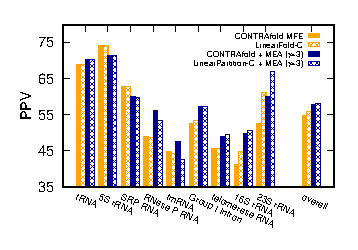
\includegraphics[width=.45\textwidth]{figs/MEA_vs_MFE_PPV_LPC}
    &
    \hspace{-0.1cm}
    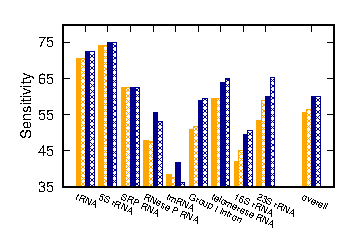
\includegraphics[width=.45\textwidth]{figs/MEA_vs_MFE_sens_LPC}
  \end{tabular} \\[-0.5cm]
  \caption{Accuracy comparison of MEA structures ($\gamma=3$) between \contrafold and \linearpartitionc on the ArchiveII dataset. 
  $\gamma$ is the hyperparameter balances PPV and Sensitivity. Note that \linearpartitionc + MEA is significantly worse than \contrafold + MEA on two families in both PPV and Sensitivity, tmRNA and RNase P RNA ($p < 0.01$).
  \label{fig:mea_lpc}}
%\vspace{1cm}
\end{figure}
\fi

% threshknot
\iftrue
\begin{figure}[h]
  \centering
%\hspace{-0.5cm}
\begin{tabular}{ll}
{\large\sf A} & {\large\sf B}\\[-1cm]
    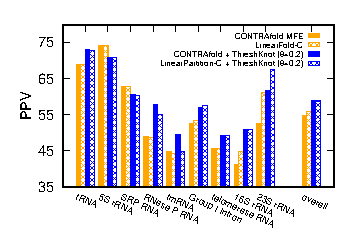
\includegraphics[width=.45\textwidth]{figs/new_ThreshKnot_vs_MFE_PPV_LPC}
    &
    \hspace{-0.1cm}
    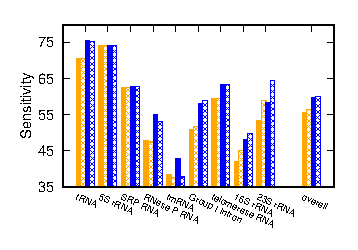
\includegraphics[width=.45\textwidth]{figs/new_ThreshKnot_vs_MFE_sens_LPC}
  \end{tabular} \\[-0.5cm]
  \caption{Accuracy comparison of ThreshKnot structure ($\theta=0.2$) between \contrafold and \linearpartitionc on ArchiveII dataset. $\theta$ is the hyperparameter that balances PPV and Sensitivity. Note that \linearpartitionc + ThreshKnot is significantly worse than \contrafold + ThreshKnot on two families in both PPV and Sensitivity, tmRNA and RNase P RNA ($p < 0.01$), and significantly better on three longer families in Sensitivity, Group I Intron ($p < 0.01$), telomerase RNA and 16S rRNA ($0.01 \leq p < 0.05$).
  \label{fig:threshknot_lpc}}
%\vspace{1cm}
\end{figure}
\fi


\begin{figure}[h]
  \centering
  \captionsetup{singlelinecheck=off}
\begin{tabular}{cc}
\hspace{-6.cm} \panel{A} & \hspace{-6cm}\panel{B} \\[-0.5cm]%& \hspace{-4.6cm}\panel{C} & \hspace{-4.6cm}\panel{D}\\[-0.2cm]
\hspace{-0.2cm}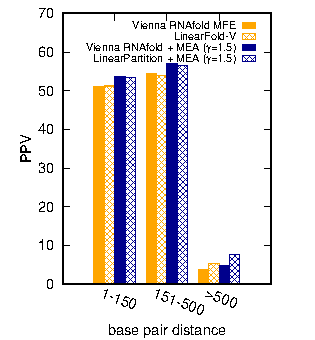
\includegraphics[width=0.35\textwidth]{figs/bylen_bar_precision_hzhang} &
\hspace{-0.35cm}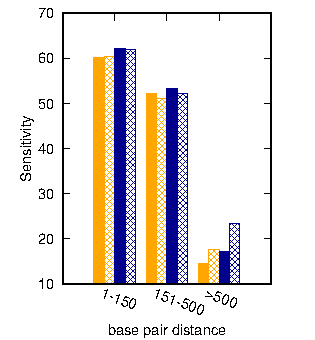
\includegraphics[width=0.35\textwidth]{figs/bylen_bar_recall_hzhang} \\
\hspace{-6.cm} \panel{C} & \hspace{-6cm}\panel{D} \\[-0.5cm]
\hspace{-0.35cm}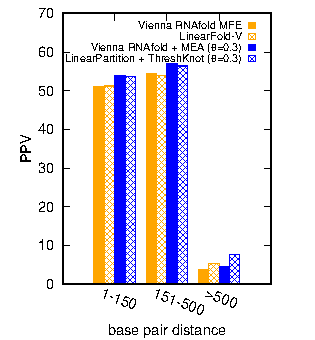
\includegraphics[width=0.35\textwidth]{figs/bylen_bar_precision_hzhang_threshknot} &
\hspace{-0.35cm}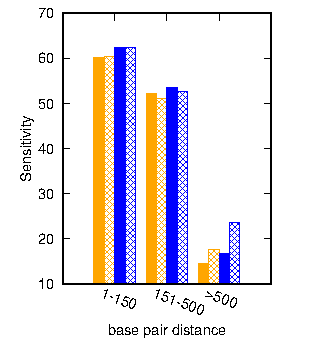
\includegraphics[width=0.35\textwidth]{figs/bylen_bar_recall_hzhang_threshknot}
\end{tabular}
  \caption[.]{Accuracy comparison of base pair prediction with different base pair distances. 
  Each bar represents the overall PPV/sensitivity of all predicted 
base pairs in a certain length range across all sequences. 
\linearpartition performs best on long base pairs over four systems. 
{\bf A} and {\bf B}: Comparison using MEA structures. 
{\bf C} and {\bf D}: Comparison using \threshknot structures.
In all cases, \linearpartition's base pair probabilities lead to substantially better accuracies on long-distance pairs (500+ \nts apart).
  \label{fig:distance}}
%\vspace{1cm}
\end{figure}


\iftrue
\begin{figure}[h]
  \centering
%\hspace{-0.5cm}
\begin{tabular}{ll}
{\large\sf A} & {\large\sf B}\\
    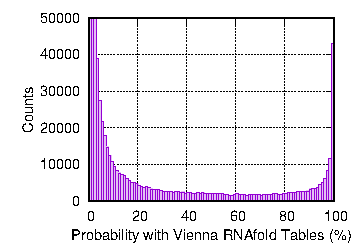
\includegraphics[width=.45\textwidth]{figs/overall_vienna_prob_bin_count}
    &
    \hspace{-0.1cm}
    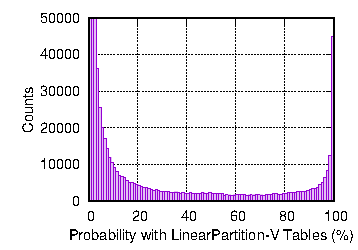
\includegraphics[width=.45\textwidth]{figs/overall_lpv_prob_bin_count}
  \end{tabular} 
  \caption{Pair probability distributions of \viennarnafold and \linearpartitionv are similar.
  {\bf A}: 
  Pair probability distribution of \viennarnafold;
  {\bf B}: 
  Pair probability distribution of \linearpartitionv.
  The count of \linearpartitionv in bin [99,100) is slightly bigger than \viennarnafold, 
  while the count in bin [0,1) (cut here at 50,000) is much less than \viennarnafold 
  (2,068,758 for \linearpartitionv and 48,382,357 for \viennarnafold).
  % This comparison also confirm that \linearpartition prune out lots of base pairs with probabilities close to 0, and the base pairing probability distribution of \linearpartition is peakier.
  \label{fig:bin_counts}}
%\vspace{1cm}
\end{figure}
\fi

% \vspace{-0.6cm}
% \section*{References}
% \balance
% % \bibliographystyle{elsarticle-harv} % can't use any; already used unsrt in pnas-new.cls
% \bibliography{si}






%\includepdf[pages=-]{si.pdf}

\end{document}
